
\def\>{\rangle}
\def\<{\langle}

%\DeclareMathOperator{\mix}{mix}
%\DeclareMathOperator{\component}{comp}
%\DeclareMathOperator{\cospan}{cospan}
\newcommand\mix{\mathrm{mix}}
\newcommand\component{\mathrm{comp}}
\newcommand\cospan{\mathrm{cospan}}
\newcommand\dist{\mathrm{dist}}
\newcommand\hull{\mathrm{hull}}
\newcommand\support{\mathrm{supp}}
\newcommand\capacity{\mathrm{scap}}
\newcommand\size{\mathrm{frac}}
\newcommand\fcap{\mathrm{fcap}}

\newcommand\vspan{\mathrm{span}}
\newcommand\cl{\mathrm{cl}}

\def\separate{\downmodels}
\def\nseparate{\ndownmodels}
\def\ortho{\perp}

\newcommand{\ens}[1][e] {\mathsf{#1}} % Ensemble
\newcommand{\Ens}[1][E] {\mathcal{#1}} % Ensemble space

\chapter{Ensemble spaces}

In this chapter we aim to develop a general theory of states and processes that is applicable to any physical system. The core concept is that of an ensemble, and the goal is to find necessary requirements for ensembles that can serve as basic axioms and then further suitable assumptions to recover the different theories (e.g. classical, quantum or thermodynamics).

The basic premise is that physical theories are primarily about ensembles. At a practical level, most of the time we can only prepare and measure statistical properties as we do not have perfect control over any system (i.e. all measurements are really statistical). The cases where properties can be prepared with one hundred percent reliability can still be understood as ensembles of identical preparations. At a conceptual level, the goal of physics is to write laws that apply all the time: every time that one prepares a system according to a particular procedure and lets it evolve in particular conditions, he will obtain a particular result. That is, the idea of repeatability of experimental results implicitly assumes that the objects of scientific inquiry are not single instances, but the infinite collections of all reproducible instances. This means that any physical theory, at the very least, will have to provide a mathematical representation for its ensembles.

By ensemble we mean what is usually meant in statistical mechanics: we have a preparation device that follows some known recipe; its output is varied but it is consistently varied (i.e. its statistical properties are well defined); the collection of all possible outputs taken as one object is an ensemble. In classical physics, ensembles are probability distributions over the full description of the system, over phase space for classical mechanics. In quantum mechanics, ensembles are represented by density matrices and density operators. In the standard approach statistical ensembles are defined on top of the space of ``true'' physical states (e.g. microstates, pure states, ...). We will proceed in the opposite way: we will start from the ensembles and recover the states as the ``most pure'' ensembles. There are two main advantages: the first is that we can create a theory that is agnostic about what the fundamental states are, and is therefore general. The second is that this approach is more in line with experimental practice: the experimental data is about statistical ensembles only and the pure states are idealizations that are useful as a mental model or for calculation.

There are three main requirements for ensembles. First, they must be experimentally well defined. This means that there need to be enough experimentally verifiable statements and experimental tests to fully characterize them. This will impose a topology on the ensemble space. Second, we can always perform statistical mixtures: given two ensembles, we can create a third one by selecting the first or the second according to a certain probability. This will impose a convex structure on the ensemble space. Third, ensembles will need a well-defined entropy which quantifies the variability of the elements within the ensemble. Since the variability cannot decrease when performing a statistical mixture and can only increase up to the variability introduced by the selection, the entropy will have to satisfy certain bounds.

From these axioms, many general results can be proven. An ensemble space will be a convex subset of a vector space that will extend over a bounded interval in each direction. The concavity of the entropy will impose a metric over the space, turning it into a geometric space and a metrizable topological space. Each ensemble can be characterized by a sub-additive measure, which becomes a probability measure in the classical case. This makes the space of physical theories a lot more constrained than one may imagine at first.

Note: all $\log$s are assumed to be in base 2.

\section{Review of standard cases}

We will start this chapter by reviewing three cases: discrete classical ensembles, continuous classical ensembles and quantum ensembles. These will be useful both to form an intuition for ensembles and to serve as targets that the whole theory needs to reproduce. We will also go though a series of problematic details and exceptions that we will need to address in the development of the general theory.

\subsection{Discrete classical ensemble spaces}

\begin{defn}
	A \textbf{discrete classical ensemble space} is the space of probability distributions over a countable number of cases. That is, a discrete classical ensemble space is the simplex $\Ens$ containing $n$ points, possibly countably infinite, $\{s_i\}^n_{i=1}$ and for which every element $\ens \in \Ens$ is characterized by a unique convex combination $\ens = \sum_i p_i s_i$ such that $\sum_i p_i = 1$. The space is closed under convex combinations of finitely many elements. The entropy is given by $S(\ens) = - \sum_i p_i \log p_i$.
\end{defn}

\subsubsection{Finite case}

The space of classical distributions over a discrete space corresponds to a \href{https://en.wikipedia.org/wiki/Simplex}{simplex}. In the finite case, the pure states $\mathcal{S} = \{s_i\}_{i=1}^{n} \subset \Ens$ are finitely many and each ensemble $\ens = \sum_i p_i s_i$ is uniquely identified by a decomposition of pure states. Effectively, each ensemble is a probability distribution over the pure states. Mathematically, each point of the space is a convex combination of the vertices. The simplex has a center point, which corresponds to the maximally mixed state, a uniform distribution over all pure states. 

The entropy is given by the Shannon entropy $-\sum_i p_i \log p_i$. This means that the entropy of each pure state is zero and the entropy of the maximally mixed state is $\log n$ where $n$ is the number of pure states. The entropy increases as we go from pure states to the maximally mixed state. The level sets (i.e. the fibers) of the entropy form a series of concentric ``shells''.

Note that imposing zero entropy on all pure states is a restrictive condition that does not apply in general. To see this, consider the case where the state is defined by the number of molecules for two substances. This space is the product of two independent variables $n_a$ and $n_b$. If we have a uniform distribution over $N_a$ cases of $n_a$ and $N_b$ cases of $n_b$, the total number of cases is $N_a N_b$. Therefore the entropy of the joint state is the sum of the entropy of the marginals. However, if we pair $n_a$ with the total number of molecules $n_{(a+b)}$ we have a problem. The issue is that the variable $n_{(a+b)}$ corresponds to a variable number of joint cases. Therefore the case where the ensemble space is a simplex but the entropy is not the Shannon entropy (i.e. is the Shannon entropy plus the contributions of entropy from each vertex) is a physically meaningful case that should be possible in the general theory.

\subsubsection{Countable case}

The countable case is, in some respects, not well defined.

The obvious extension is to include all sequences $\{p_i\} \in [0,1]$ whose sum converges to one (i.e. the space of all probability measures over a countable discrete space). Since we cannot create a uniform distribution over infinitely many cases, there is no center point, there is no barycenter. Effectively, there is a ``hole'' in the middle.\footnote{It may be useful to characterize this ``hole'' and the limit points. There should be at least one limit point for each sequence $\{p_i\}$ whose sum converges to a finite $p < 1$. Intuitively, we can keep that part of the distribution constant while we spread the rest uniformly to all other cases. Each should reach a different limit point.}

However, the space of all probability measures is too large. Note that the entropy is not finite for all $\sum_i p_i =1$ (i.e. infinite convex combinations). For details, see \href{https://arxiv.org/pdf/1212.5630.pdf}{this article}. Given that we want the entropy to exist and be finite for all ensembles, this generalization (like the one provided \href{https://ncatlab.org/nlab/show/superconvex+space}{here}) does not seem physically warranted.

Also note that expectation values are not guaranteed to be finite either, and requiring a particular observable to be finite further restricts the space. This restriction may be desirable for another reason: a discrete ensemble space has no notion of the ordering of the pure states. Physically, this would mean that the states with 1, 100, or 1 trillion particles are ``equally distant'' (i.e. all infinite permutations are allowed). Requiring the expectation of the number of particles to be finite (e.g. $\sum_i N(i) p_i < \infty$) should effectively encode the infinite ordering in the rate of convergence of the probability distributions (i.e. not all infinite permutations would be allowed).

\subsubsection{No uncountable case}

The uncountably infinite case is not physically relevant (i.e. no second countable discrete topology, cases are not experimentally decidable). Also note that any set of real numbers whose sum is finite can have only countably many non-zero elements. To understand why, note that there can only be finitely many terms above any particular positive value if their sum is to remain finite. Effectively, the uncountable case would be stitching together infinitely many countable cases.

\subsection{Continuous classical ensemble spaces}

\begin{defn}
	A \textbf{continuous classical ensemble space} is the space of probability distributions over phase space. That is, it is the space of probability measures over a symplectic manifold that is absolutely continuous with respect to the Liouville measure. The entropy is given by the Shannon/Gibbs entropy calculated using the probability density (i.e. the Radon-Nikodym derivative between the probability measure $p$ and the Liouville measure $\mu$). That is, $S(\rho) = - \int_X \rho \log \rho d\mu$ where $\rho = \frac{dp}{d\mu}$.
\end{defn}

In the continuous case, the space of ensembles is the space of integrable functions over a symplectic manifold (e.g.  over phase space) that integrate to one. That is, if $X$ is a symplectic manifold, then $\Ens = \{ \rho \in L^1(X) \, | \, \int_X \rho(x) d\mu = 1 \} $ where $\mu(U)=\int_U \omega^n$ is the Liouville measure. There are no extreme points in the convex space, meaning there are no ensembles that cannot be written as a convex combination of other ensembles. This is important as, when developing standard constructions in the ensemble space, one cannot rely on the existence of extreme points.

The delta distributions are not part of the space. In fact, the relative measures are not absolutely continuous with respect to the Liouville measure (i.e. they assign non-zero probability over a set of measure zero). Therefore one should not think of delta distributions as ``pure states.'' There is a difference between the spectra (i.e. the possible values of a random variable) and states, which will be even more pronounced in the quantum case.

The symplectic nature of the manifold is required to assign a frame-invariant density to states and a frame-invariant notion of independence between DOFs, as we saw in the classical mechanics section of reverse physics.

The entropy is given by $- \int \rho \log \rho d\mu$ where $\mu$ is the Liouville measure and $\rho$ is the probability density over canonical coordinates. If a different measure is used, or if the coordinates are not canonical, the formula gives the wrong result.\footnote{It may be interesting to study the shell of zero entropy states. For example, it should not be path connected. All uniform distributions with support of the same finite size (in terms of the Liouville measure) will have the same entropy. The region, however, need not be contiguous. Since we cannot continuously transform a single region into two disjoint regions, there will be different distributions at zero entropy that cannot be transformed continuously.}


Similarly to the countable discrete case, the entropy can be infinite and expectation values can be infinite. The added complication is the frame invariance: it would not make sense to have the expectation for position in one frame to be finite while infinite in another. Requiring all functions of position and momentum to have finite expectations restricts the distributions to those with finite support. Requiring all polynomial functions of position and momentum to have finite expectation restricts the distributions to those that decay faster than any polynomial.

Unlike the discrete classical case, subspaces and dimensionality of subspaces cannot be defined without the entropy. The issue is that we need a measure on the set of pure states, and the convex structure cannot provide it. The entropy, however, does as the supremum of the entropy for all distributions with support $U$ is $\log \mu(U)$. As we will see, the entropy can be used to both identify subspaces and recover the Liouville measure.

It is a bit unclear whether discontinuous distributions should be included or not. Originally, we thought the probability density should be continuous as only continuous functions can physically represent experimental relationships. However, the relationship given by the measure is not between points and probability but rather between sets and probability. The probability density is, in a sense, not the prime physical object. The measure is. The probability density, in fact, is not uniquely defined as countably many discontinuities can be added and the measure is not changed.

\subsection{Quantum ensemble spaces}

\begin{defn}
	A \textbf{quantum ensemble space} is the space given by the density matrices/operators of a Hilbert space equipped with the von Neumann entropy. That is, given a separable Hilbert space $\mathcal{H}$ representing a quantum system, the ensemble space is the space of positive semi-definite self-adjoint operators with trace one $M(\mathcal{H})$. The space of pure states is given by the projective space $P(\mathcal{H})$. The entropy of an ensemble $\rho \in M(\mathcal{H})$ is given by the von Neumann entropy $S(\rho) = -\tr(\rho \log \rho)$.
\end{defn}

\subsubsection{Finite dimensional case}

The simplest non-trivial case is the qubit, for which the Bloch ball is the space of ensembles $M(\mathcal{H})$. The interior of the Bloch ball corresponds to mixtures  while the surface corresponds to the pure states $\mathcal{S} = P(\mathcal{H}) = \{ |\psi\> \<\psi| \}_{\psi \in \mathcal{H}}$. In quantum ensemble spaces there is no unique decomposition in terms of pure states. Note that the space is exactly characterized by knowing which different mixtures provide the same ensemble.

The multiple decompositions make the ensemble space behave in a way that is a hybrid between the classical discrete and continuous. Pure states are properly a part of the ensemble space, as in the discrete case, and we can describe each mixture in terms of finitely many pure states. However, the pure states form a continuum, therefore we can also define probability densities over the space, convex integrals. For example, for a single qubit, the maximally mixed state (the center of the ball) can be equally described as the equal mixture of two opposite states (e.g. spin up and spin down, or spin left and spin right). However, it can also be described as the equal mixture of the whole sphere.

Note that complex projective spaces are symplectic, which is what allows one to define frame invariant densities. The goal is to have one argument applied to the generic definition as to why the space of pure states must be symplectic. Also note that the two dimensional sphere is the only symplectic sphere. By homogeneity, we should be able to argue that the space is symmetric around the maximally mixed state, and is therefore a sphere. The symplectic requirement would select dimension two. Note that real and quaternionic spaces would be excluded by this argument.

The von Neumann entropy for the maximally mixed state is $\log n$ where $n$ is the dimensionality of the Hilbert space. Again we see that the maximum entropy gives us a measure of the size of the space. Note that, to calculate the von Neumann entropy, we are diagonalizing the density matrix $\rho$. This means finding a set of orthogonal pure states $s_i$ such that $\rho = \sum p_i s_i$ is a convex combination. Note that the convex hull of a set of $n$ orthogonal pure states is an $n$-dimensional simplex whose center is the maximally mixed state. Therefore, we are looking for a simplex that contains $\rho$ and the maximally mixed state. In the two dimensional case, $\rho$ is an interior point of the Bloch ball. Take the line that connects $\rho$ to the center. The two points of the sphere are the extreme points for the decomposition. The distance from the points will be proportional to the probability. Because of this property, the von Neumann entropy is the smallest Shannon entropy between all possible decompositions.


\subsection{Countably infinite dimensional case}

The countable infinite dimensional case presents similar problems as the classical case, and adds others. As in the classical infinite cases, the maximally mixed state (i.e. uniform distribution) is not in the convex space and the entropy is not finite for all infinite convex combinations. As in the classical continuous case, there is the issue of finite expectation of position/momentum in all frames. The problem is compounded by the fact that one cannot require finite expectation for all functions of position and momentum: finite support in position automatically implies infinite support on momentum, since the distribution in momentum is the Fourier transform of that in position.

The Hilbert space for a discrete variable with infinite range (e.g. number of particles) and a continuous variable (e.g. position/momentum) is the same. The first is defined as the space of square convergent complex sequences $l^2$ while the second is the space of square integrable complex functions $L^2$. Given that $L^2$ allows a countable basis, the two are isomorphic. This also means that all spaces with finitely many degrees of freedom are also isomorphic. This makes the problem of infinite expectations even more problematic.

Note that Schwartz spaces have finite expectation for all polynomial functions of position and momentum. Given that infinite permutations can change the rate of convergence, the Schwartz space has an idea of what is further away from the origin, unlike Hilbert spaces. We will likely want to use Schwartz spaces instead of Hilbert spaces to make the physics and mathematics more consistent.

\section{Axiom of ensemble and topology}

The first property of ensembles is that they must be experimentally well-defined. As shown in the previous chapters, this means that they are possibilities of an experimental domain, which means points of a $\textsf{T}_0$ second countable topological space where the topology corresponds to the natural one defined by the verifiable statements.

The verifiable statements for the ensemble space are statements about the ensembles themselves, either in terms of statistical quantities (e.g. \statement{the average energy is of the particle is $3 eV \pm 0.5$}) or in terms of preparation settings (e.g. \statement{the beam goes through a polarizer oriented to the vertical direction within 1 degree}). Probability ranges are also typical verifiable statements on ensembles (e.g. \statement{the coin toss will result in heads between 49 and 51 percent of the cases}). The verifiable statements on the specific instances will be recovered later from the structure of the ensemble space as we recover probability distributions of specific quantities. The topology of the two is related but it is not the same (e.g. the topology of the Bloch ball is the standard topology of $\mathbb{R}$ but the topology on the values of an observable is the discrete topology).

The fact that we start from ensembles and recover the probability of outcomes, instead of constructing ensembles from the probability of outcomes, should avoid the problems associated with frequentist interpretations of probability.

\begin{mathSection}
	\begin{axiom}[Axiom of ensemble] 
		The state of a system is represented by an \textbf{ensemble}, which represents all possible preparations of equivalent systems prepared according to the same procedure. The set of all possible ensembles for a particular system is an \textbf{ensemble space}. Formally, an ensemble space is a $T_0$ second countable topological space where each element is called an ensemble.
	\end{axiom}
	
	\begin{justification}
		In experimental setting, preparation procedures never prepare a system exactly in the same configuration. Experimental results, then, are always in terms of statistical preparations and statistical measurements. A physical theory, then, must be able to talk about what are the possible statistical ensembles describable by the theory. States, then, can be understood as ensembles as those are what we produce and study in practice.
		
		Equivalently, reproducibility is a basic requirement of a physical theory. A physical law, then, must be understood as describing a relationship that always exists whenever the same set of circumstances is replicated. Given that we need to always be able to replicate those circumstances ``one more time'', the relationship is about countably infinite preparations and results: ensembles. Therefore, to the extent that physics is about reproducible experimental results, the basic description of a system is in terms of ensembles. This justifies the use of ensembles as the fundamental object to describe the state of a system.\footnote{Note that reproducibility also already implies that all properties that characterize an ensemble must be relative to the procedure. If the properties depended, for example, on absolute space or absolute time, then different practitioners would not be able to prepare the same ensemble.}
		
		Ensembles are experimentally defined objects, and therefore they are possibilities of an experimental domain. Therefore an ensemble space is a $T_0$ second countable topological space where each element is an ensemble and the topology is induced by the verifiable statements.
	\end{justification}
\end{mathSection}

We should now verify that our three basic cases satisfy the axiom of ensemble.

\begin{prop}
	Classical discrete, classical continuous and quantum ensemble spaces satisfy the axiom of ensemble.
\end{prop}

\begin{proof}
	For the classical discrete case, including all infinite convex combinations, we have $\ell^1$. Similarly, for the classical continuous case we have $L^1$. Both of these spaces are separable, admit a countable orthonormal basis and can be given a topology that is $\textsf{T}_0$ and second countable.
	
	For the quantum case, the Hilbert space is also separable, will admit a countable orthonormal basis and can be given a topology that is $\textsf{T}_0$ and second countable. An operator will be fully defined by its result on the basis, which means that it is also a vector space with a countable basis and can be given a topology that is $\textsf{T}_0$ and second countable.
\end{proof}

\section{Axiom of mixture and convex spaces}

The second property of ensembles is that they can be mixed. That is, we can take two preparation procedures and choose between them with a known probability. This constitutes another ensemble. The convex space structure is ultimately responsible for all linear structures in physics.

\begin{defn}
	Given a real number $p \in [0,1]$, its complement is defined as $\bar{p} = 1-p$.
\end{defn}

\begin{axiom}[Axiom of mixture]
	An ensemble space is closed under statistical mixing. Formally, an ensemble space $\Ens$ is equipped with an operation $+ : [0, 1] \times \Ens \times \Ens \to \Ens$ called \textbf{mixing}, noted with the infix notation $p \ens[a] + \bar{p} \ens[b]$, with the following properties:
	\begin{itemize}
		\item \textbf{Continuity}: the map $+(p, \ens[a], \ens[b])  \to p \ens[a] + \bar{p} \ens[b]$ is continuous (with respect to the product topology $[0, 1] \times \Ens \times \Ens$)
		\item \textbf{Identity}: $1 \ens[a] + 0 \ens[b] = \ens[a]$
		\item \textbf{Idempotence}:  $p \ens[a] + \bar{p} \ens[a] = \ens[a]$ for all $p \in [0,1]$
		\item \textbf{Commutativity}: $p \ens[a] + \bar{p} \ens[b] = \bar{p} \ens[b] + p \ens[a]$ for all $p \in [0,1]$
		\item \textbf{Associativity}: $p_1 \ens_1 + \bar{p}_1\left(\overline{\left(\frac{p_3}{\bar{p}_1}\right)}\ens_2 + \frac{p_3}{\bar{p}_1}\ens_3\right) =  \bar{p}_3\left(\frac{p_1}{\bar{p}_3} \ens_1 +  \overline{\left(\frac{p_1}{\bar{p}_3}\right)}\ens_2\right) + p_3 \ens_3$ where $0 < p_1 + p_3 < 1$
	\end{itemize}
\end{axiom}

\begin{justification}
	This axiom captures the ability to create a mixture merely by selecting between the output of different processes. Let $\ens_1$ and $\ens_2$ be two ensembles that represent the output of two different processes $P_1$ and $P_2$. Let a selector $S_p$ be a process that outputs two symbols, the first with probability $p$ and the second with probability $\bar{p}$. Then we can create another process $P$ that, depending on the selector, outputs either the output of $P_1$ or $P_2$. All possible preparations of such a procedure will form an ensemble. Therefore we are justified in equipping an ensemble space with a mixing operation that take a real number from zero to one and two ensembles.
	
	Given that mixing represents an experimental relationship, and all experimental relationships must be continuous in the natural topology, mixing must be a continuous function. Note that $p$ is a continuously ordered quantity, where no value is perfectly experimentally verifiable, and therefore the natural topology is the one of the reals. This justifies continuity.

	If $p=1$, the output of $P$ will always be the output of $P_1$. This justifies the identity property. If $P_1$ and $P_2$ are the same process, then the output of $P$ will always be the output of $P_1$. This justifies the idempotence property. The order in which the processes are given does not matter as long as the same probability is matched to the same process. The process $P$ is identical under permutation of $P_1$ and $P_2$. This justifies commutativity. If we are mixing three processes $P_1$, $P_2$ and $P_3$, as long as the final probabilities are the same, it does not matter if we mix $P_1$ and $P_2$ first or $P_2$ and $P_3$. This justifies associativity.
\end{justification}

\begin{remark}
	Given commutativity and associativity, we can write $p_1 \ens[a] + p_2 \ens[b] + p_3 \ens_3$ where $p_2 = \bar{p}_1\overline{\left(\frac{p_3}{\bar{p}_1}\right)} = \bar{p}_3\overline{\left(\frac{p_1}{\bar{p}_3}\right)} = 1 - p_1 - p_3 = \overline{\left(p_1 + p_3\right)}$.
	
	We can also extend to mixtures of finitely many elements $\sum_{n=1}^\infty p_i \ens_i$ where $\sum_{n=1}^\infty p_i = 1$ with the following caveat. The mixture is guaranteed to exist only for finitely many elements. Whether an infinite sum $\sum_{i=1}^\infty \ens_i$ converges or not in the space is determined by the topology (i.e. experimental verifiability). The goal is to work with only finite convex combinations and let the closure of the topology handle the limits.
\end{remark}

\begin{coro}
	An ensemble space is a convex space.
\end{coro}

\begin{proof}
	The properties of the axiom of mixture match the basic definition of a convex spaces, which can be taken from \href{https://ncatlab.org/nlab/show/convex+space}{ncatlab} and \href{https://arxiv.org/abs/0903.5522}{this excellent paper}.  The notation and terminology will be slightly different to better map to physics ideas. 
\end{proof}

\begin{prop}
	Discrete classical ensemble spaces, continuous classical ensemble spaces and quantum ensemble spaces satisfy the axiom of mixture.
\end{prop}

\begin{proof}
	The space of probability measures, discrete or continuous, $\Ens$ is a convex subset of the vector space of signed finite measures. It is therefore closed under convex combinations: if $\{e_i\} \subseteq \Ens$ are probability measure, then $\sum p_i \ens_i$ with $\sum p_i = 1$ is a probability measure. The properties of mixing are inherited from the properties of linear combinations. Therefore the discrete and continuous classical ensemble spaces satisfy the axiom of mixture.
	
	Similarly, the space of positive semi-definite self-adjoint operators with trace one is a convex subset of the vector space of self-adjoint operators. Therefore it is closed under convex combinations and it will satisfy the axiom of mixture.
\end{proof}

\subsection{Common components and separateness}

The convex structure allows us to characterize ensembles based on whether they can be mixed into one another. For example, we can ask whether an ensemble is or is not the mixture of some other ensembles; whether two ensembles can be expressed as a mixture of a common component.

\begin{defn}
	Let $\Ens$ be an ensemble space. Let $\ens[a] = \sum_i p_i \ens_i$ where $\ens[a], \{\ens_i\} \in \Ens$ and $p_i \in (0,1]$ such that $\sum p_i = 1$. We say that $\ens[a]$ is a \textbf{mixture} of $\{\ens_i\}$, each $\ens_i$ is a \textbf{component} of $\ens[a]$ and each $p_i$ is a \textbf{mixture coefficient}.
\end{defn}

\begin{figure}[h]
	\centering
	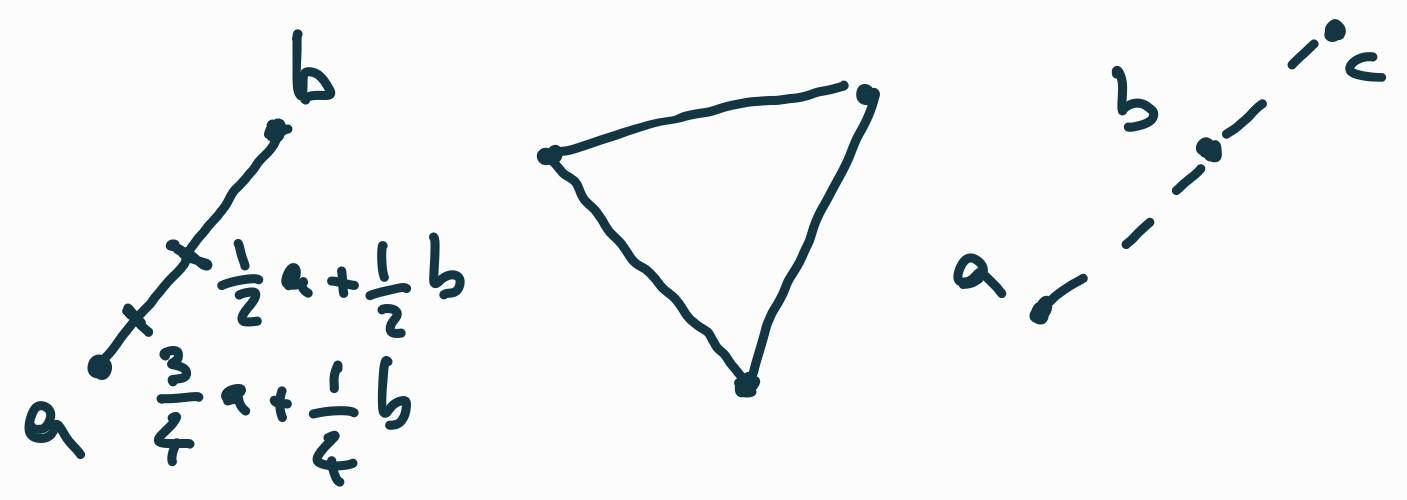
\includegraphics[width=0.5\textwidth]{tempimages/ConvexExamples.jpg}
\end{figure}

\begin{remark}
	In terms of the convex space, all the mixtures between two ensembles correspond to the segment between them; all the mixtures between three ensemble correspond to the triangle formed by the three elements and so on. An ensemble $\ens[a]$ is a component of a different ensemble $\ens[b]$ if the segment can be continued on the side of $\ens[b]$. If two elements are not a component of each other, then they are the extreme points of the line that connect the two. That is, the segment cannot be extended.
\end{remark}

\begin{figure}[h]
	\centering
	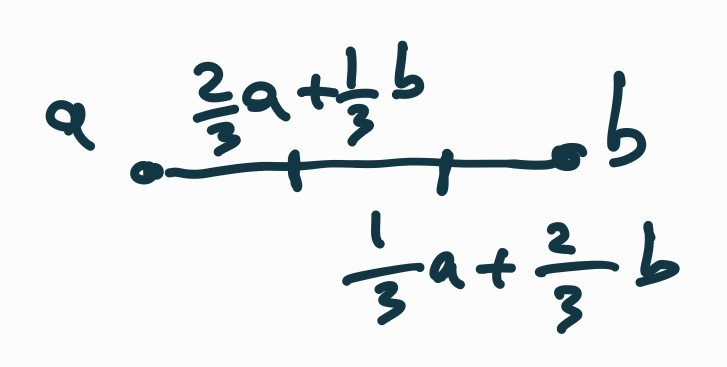
\includegraphics[width=0.5\textwidth]{tempimages/ComponentNotOrder.jpg}
\end{figure}

\begin{remark}
	Note that two ensembles can be the component of each other. Consider $\frac{2}{3} \ens[a] + \frac{1}{3} \ens[b]$ and $\frac{1}{3} \ens[a] + \frac{2}{3} \ens[b]$. We can write $\frac{2}{3} \ens[a] + \frac{1}{3} \ens[b] = \frac{1}{2}\left(\frac{1}{3} \ens[a] + \frac{2}{3} \ens[b]\right) + \frac{1}{2} \ens[a]$ and $\frac{1}{3} \ens[a] + \frac{2}{3} \ens[b] = \frac{1}{2}\left(\frac{2}{3} \ens[a] + \frac{1}{3} \ens[b]\right) + \frac{1}{2} \ens[b]$ (they are both midpoints along each other). Therefore a component is not necessarily ``smaller'' or ``better defined'' than the mixture. Mathematically, ``being a component of'' is not a partial order. It is reflexive and transitive, but it is not antisymmetric. In practical term, we need something else to tell us whether we are, for example, taking a limit with components that become ``smaller and smaller.''
\end{remark}

\begin{defn}
	Let $\Ens$ be an ensemble space and $\ens[a], \ens[b] \in \Ens$. We say that they \textbf{have a common component} if we can find $\ens[c] \in \Ens$, the common component, such that $\ens[a] = p_1 \ens[c] + \bar{p}_1 \ens_a$ and $\ens[b] = p_2 \ens[c] + \bar{p}_2 \ens_2$ for some $\ens_1, \ens_2 \in \Ens$ and $p_1, p_2 \in (0,1)$. Otherwise, we say they \textbf{have no common component}, or are \textbf{separate}, noted $\ens[a] \separate \ens[b]$. Two ensemble have a common component in $A \subseteq \Ens$ if the common component can be found in $A$, and are separate in $A$ if there is none.
\end{defn}

\begin{figure}[h]
	\centering
	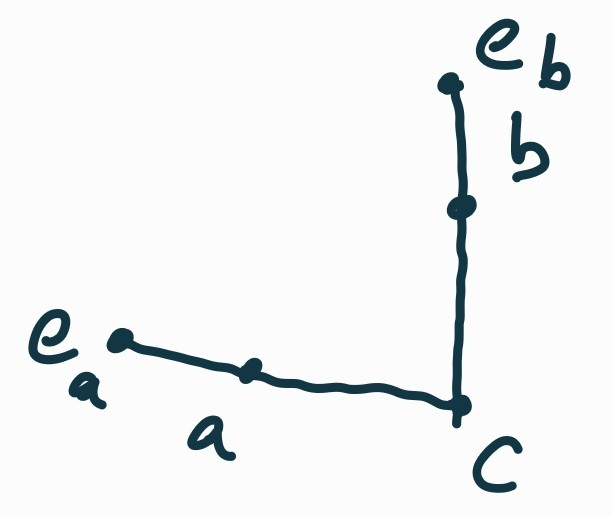
\includegraphics[width=0.5\textwidth]{tempimages/CommonComponent.jpg}
\end{figure}

\begin{remark}
	If two ensembles $\ens[a]$ and $\ens[b]$ have a common component $\ens[c]$, then the ensemble space contains a triangle where $\ens[c]$ is a vertex and $\ens[a]$ and $\ens[b]$ are points on the sides that connect to $\ens[c]$.
\end{remark}

\begin{coro}
	The previous definitions obey the following:
	\begin{enumerate}
		\item every ensemble has a common component with itself, therefore every ensemble is not separate from itself
		\item separateness is an irreflexive symmetric relation
		\item if $\ens[a]$ is a component of $\ens[b]$, then $\ens[a]$ and $\ens[b]$ have a common component
	\end{enumerate}
\end{coro}

\begin{proof}
	1. Since by idempotence $\ens = p \ens + \bar{p} \ens$ for any $p$, we can satisfy the definition by setting $\ens[a] = \ens[b] = \ens[c] = \ens_1 = \ens_2 = \ens$. Therefore every ensemble has a common component with itself and every ensemble is not separate from itself.
	
	2. The previous property shows that separateness is irreflexive. The definition of common component is symmetric and therefore so is separateness.
	
	3. By idempotence, we can write $\ens[a] = p_1 \ens[a] + \bar{p_1} \ens[a]$ for some $p_1 \in (0,1)$. Since $\ens[a]$ is a component of $\ens[b]$, we can write $\ens[b] = p_2 \ens[a] + \bar{p_2} \ens[c]$ for some $p_2 \in (0, 1)$ and $\ens[c] \in \Ens$. Therefore $\ens[a]$ and $\ens[b]$ have a common component.
\end{proof}

\subsection{Convex subsets and convex hull}

\begin{defn}
	Let $\Ens$ be an ensemble space. We say $A \subseteq \Ens$ is a \textbf{convex subset} of $\Ens$ if it is closed under mixture and it is a closed set. That is, it contains all possible mixtures that can be constructed form its elements, including infinite ones. If we want to stress that we care closing only under finite mixing, we say that $A$ is closed under finite convex combinations.
\end{defn}

\begin{defn}
	Let $A \subseteq \Ens$ be a subset of an ensemble space. The \textbf{convex hull} of $A$, noted $\hull(A)$ is the set of all possible mixtures that can be constructed with elements contained in $A$, including infinite ones. That is, it is the topological closure of the closure of $A$ under mixing.
\end{defn}

\begin{coro}\label{pm_es_hullProp}
	The convex hull has the following properties
	\begin{enumerate}
		\item $A \subseteq \hull(A)$
		\item $A \subseteq B \implies \hull(A) \subseteq \hull(B)$
		\item $\hull(\hull(A)) = \hull(A)$
	\end{enumerate}
	and is therefore a closure operation
\end{coro}

\begin{proof}
	1. Every element of $A$ is trivially a mixture of elements of $A$. Therefore $A \subseteq \hull(A)$.
	
	2. Let $\ens \in \hull(A)$. Then it is a mixture of some elements of $A$. Since $A \subseteq B$, then $\ens$ is also the mixture of some elements of $B$ and therefore $\ens \in \hull(B)$.
	
	3. Since mixing is associative and commutative, a mixture of mixtures of $U$ can be re-epressed as a mixture of $\hull(A)$. Therefore for all $\ens \in \hull(\hull(A))$ we have $\ens \in \hull(A)$.
\end{proof}

\begin{coro}
	A subset $A \subseteq \Ens$ is convex if and only if it is its own convex hull.
\end{coro}

\begin{proof}
	Let $A \subseteq \Ens$ be a convex subset. By \ref{pm_es_hullProp} we have $A \subseteq \hull(A)$. By definition of convex set, we have $\hull(A) \subseteq A$. Therefore $A = \hull(A)$. Conversely, consider let $A \subseteq \Ens$ be a set of ensembles not necessarily convex. By definition, $\hull(A)$ is closed under mixture and is therefore a convex subset.
\end{proof}

\begin{conj}
	The hull is
	\begin{enumerate}
		\item continuous from above: $\hull(\lim\limits_{i \to \infty} A_i) = \lim\limits_{i \to \infty} \hull(A_i)$ for any decreasing sequence $\{A_i\}$
		\item not continuous from below: $\hull(\lim\limits_{i \to \infty} A_i) = \lim\limits_{i \to \infty} \hull(A_i)$ for any increasing sequence $\{A_i\}$
	\end{enumerate}
\end{conj}

\begin{proof}
	It would seem that from above we are taking an infinite intersection of closed sets, which will be closed. From below, we would be taking an infinite union of closed sets, which will not be closed. We would be missing the closure of infinite convex combination with, for example, an element in each set.
\end{proof}

\begin{coro}
	The set $\mathfrak{Conv}_{\Ens}$ of all convex subsets of $\Ens$ ordered by set inclusion is a topped $\bigcap$-structure and therefore is also a complete lattice.
\end{coro}

\begin{proof}
	Let $\mathfrak{Conv}_{\Ens}$ be the set of all convex subsets of $\Ens$ ordered by set inclusion. The empty set $\emptyset \subset \Ens$ is a convex set. The whole space $\Ens \subseteq \Ens$ is also a convex set. It is therefore a bounded ordered set.
	
	Let $A, B \in \mathfrak{Conv}_{\Ens}$ be two convex subsets. Consider $A \cap B$. Any mixture of elements in $A \cap B$ is both a mixture of elements in $A$ and a mixture of elements in $B$. Therefore any mixture of elements of $A \cap B$ is both an element of $A$ and an element of $B$. This means it is also an element of $A \cap B$, which is therefore a convex set.
	
	The previous argument generalizes to a family of convex subsets $\{A_i\}_{i \in I} \subseteq \mathfrak{L}$. Moreover, the intersection of infinitely many closed sets is still closed. Therefore $\bigcap_{i \in I} A_i \in \mathfrak{Conv}_{\Ens}$ and $\mathfrak{Conv}_{\Ens}$ is an $\bigcap$-structure. This also means that it is a complete lattice.
\end{proof}

\section{Axioms of entropy}

The third and final property of ensembles is that they have a well-defined entropy. The entropy quantifies the variability of the elements within the ensembles. That is, since an ensemble represents all possible preparations of equivalent systems prepared according to the same procedure, we are asking how much those preparations are different from each other. No matter what the full description of each individual preparation may be, we can assume that their variability has some specific features. It will have to be compatible with experimental verifiability (i.e. the variability must be a continuous function with respect to the topology) and with statistical mixing (i.e. the variability cannot decrease during mixing and it maximally increase when the ensembles do not overlap). The formula for entropy can then be recovered with these very broad physically justified assumptions.

The entropic structure, in general, will constrain both the topological structure, making it metrizable, and the convex structure, making it embeddable in a vector space. The entropy is also responsible for all the geometric structure of the ensemble space.

\begin{axiom}[Axiom of entropy]
	Every element of the ensemble is associated with an \textbf{entropy} which quantifies the variability of the preparations of the ensemble. Formally, an ensemble space $\Ens$ is equipped with a function $S : \Ens \to \mathbb{R}$, defined up to a positive multiplicative constant representing the unit numerical value. The entropy has the following the following properties:
	\begin{itemize}
		\item \textbf{Continuity}\footnote{Currently, we are imposing that the entropy is continuous. There may be a chance that this requirement is redundant, as strict concavity and the upper variability bound may already impose this. We have found proofs that show that real valued convex/concave functions of real values are continuous. These proofs fail at the boundary, but the upper variability bound may fix this. Another open question is whether differentiability is also an independent requirement.}
		\item \textbf{Strict concavity}: $S(p\ens[a] + \bar{p} \ens[b]) \geq p S(\ens[a]) + \bar{p} S(\ens[b])$ with the equality holding if and only if $\ens[a] = \ens[b]$
		\item \textbf{Upper variability bound}: $S(p\ens[a] + \bar{p} \ens[b]) \leq I(p, \bar{p}) + p S(\ens[a]) + \bar{p} S(\ens[b])$; if the equality holds, $\ens[a]$ and $\ens[b]$ are \textbf{non-overlapping} or \textbf{orthogonal}, noted $\ens[a] \ortho \ens[b]$; the function $I(p_1, p_2)$ is the same for all ensemble spaces
		\item \textbf{Mixtures preserve orthogonality}:\footnote{It is unclear whether ``mixtures preserve orthogonality'' is an independent axiom. Intuitively, the following argument tells us that it is. Take the 2 dimensional simplex (i.e. a triangle) that represent a classical discrete probability space over three elements. Take the standard entropy, which will satisfy ``mixtures preserve orthogonality''. This is because the middle point has entropy $\log 3$. We can imagine changing the entropy so that it is a little bit lower in the center but it is unchanged on the sides. However, one needs to provide an actual example and show that it satisfies all axioms. It may also be that only one direction is an independent axiom. That is, that orthogonality with the components implies orthogonality with the mixtures. This is what does not hold for separateness.} $\ens[a] \ortho \ens[b]$ and $\ens[a] \ortho \ens[c]$ if and only if $\ens[a] \ortho p \ens[b] + \bar{p} \ens[c]$ for any $p \in (0,1)$
	\end{itemize}
\end{axiom}

\begin{justification}
	The entropy quantifies the variability of the instances of the ensemble. Since the ensemble represents a collection of preparations of equivalent systems, and since each instance will in general be potentially different, it is legitimate to ask how much variability there is among the different instances. We are assuming that the entropy is a quantity (i.e. a linearly ordered property), meaning that is always meaningful to tell whether one ensemble has more variability than another. If this is the case, the later requirement of continuity and strict concavity will force the entropy to be a real valued quantity. This is because the variability will change under statistical mixtures, and since statistical mixtures are performed with real valued coefficients, the variability will have to be a real valued quantity. Whether it is conceptually possible to have a characterization of variability that is not linearly ordered but still have a meaningful connection with statistical mixing is an open question, therefore we are not able to fully justify entropy's linear ordering at this time. Therefore the linear ordering of the entropy should be considered an assumption. Provided that assumptions, we are justified to assume the existence of a real valued function that returns the entropy, a measure of variability of the ensemble.
	
	Since the entropy is a real valued quantity, it will have a corresponding unit. This unit is independent from all other units, and therefore the overall structure of the ensemble space must be independent from this choice. Mathematically, the physical dimension of the unit is not captured, just its numeric value. A change of unit changes the numeric value by a multiplicative constant. Since variability is an ordered quantity, with want the change of units to respect the ordering and therefore it should be a positive multiplicative constant. This justifies that the entropy function is defined up to a positive multiplicative constant.
	
	Note that the additivity of the entropy over independent system fixes the absolute scale. If $S_{AB} = S_A + S_B$, in fact, one can't rescale all three terms by an additive factor and preserve the relationship.
	
	The variability, in the end, will have physical consequences, and it will be therefore measurable and therefore experimentally verifiable. Therefore it will have to be a topologically continuous function. Moreover, small changes in the ensemble should produce small changes in the variability, which justifies analytical continuity. We are therefore justified to assume continuity of the entropy.
	
	Suppose we have two ensembles and we perform a statistical mixture. There are going to be three source of variability: the two ensembles and the random choice at every instance. The total contribution from the original ensembles will be the average variability of the original ensembles. This is increased by the variability introduced by the random choice, which is always a positive contribution. Therefore the final variability cannot be less than the average of the original ensembles. That is, $S(p\ens[a] + \bar{p} \ens[b]) \geq p S(\ens[a]) + \bar{p} S(\ens[b])$. If we are mixing an ensemble with itself, this is equivalent to just choosing from the original ensemble, therefore the variability will not increase. Conversely, if the variability stays the same, it means that the random choice does not increase the variability, and therefore we must be choosing between equivalent ensembles. Therefore we are justified to assume that entropy is strictly concave.
	
	On the other hand, the variability cannot increase arbitrarily during mixture. The maximum variability will be given when the two ensembles are non-overlapping, when an instance of the first ensemble cannot be produced by the second ensemble. That is, a single instances is enough to determine whether we have the first ensemble or the second. In this case, the variability is increase by the variability of the random choice, which must depend only by the mixture coefficient, and not the nature of the ensembles themselves. That is, $S(p\ens[a] + \bar{p} \ens[b]) \leq I(p, \bar{p}) + p S(\ens[a]) + \bar{p} S(\ens[b])$ is the upper variability bound, which is satisfied if and only if the $\ens[a]$ and $\ens[b]$ are non-overlapping. The actual function $I$ is left unspecified, as we show in proposition \ref{pm_es_entropyUnique} is the only indicator of variability that will satisfy the axiom of entropy. This justifies the upper variability bound.
	
	Now suppose ensemble $\ens[a]$ is non-overlapping with $\ens[b]$ and $\ens[c]$. That is, an instance of $\ens[a]$ cannot ever be produced by either $\ens[b]$ and $\ens[c]$. Then an instance of $\ens[a]$ cannot either be produced by a mixture of $\ens[b]$ and $\ens[c]$, since ultimately a mixture of $\ens[b]$ and $\ens[c]$ will return an instance of one of the two. Therefore $\ens[a]$ is non-overlapping with any mixture of $\ens[b]$ and $\ens[c]$. The argument works in reverse as well: if an instance of $\ens[a]$ cannot be produced by a mixture of $\ens[b]$ and $\ens[c]$, then it cannot be produced by either. This justifies mixtures preserve orthogonality.
\end{justification}

\begin{prop}
	An ensemble is not orthogonal with itself or with its own components. Two orthogonal ensembles are separate. That is, if $\ens[a] \ortho \ens[b]$ then $\ens[a] \separate \ens[b]$
\end{prop}

\begin{proof}
	To show that every ensemble is not orthogonal to itself, let $\ens[a] \in \Ens$. We have $S(p\ens[a] + \bar{p}\ens[a]) = S(\ens[a]) < I(p,\bar{p}) + p S(\ens[a]) + \bar{p} S(\ens[a])$. Therefore $\ens[a]$ is not orthogonal to itself as it does not saturate the upper bound.
	
	To show that every ensemble is not orthogonal to its own components, let $\ens[a] = p \ens[b] + \bar{p} \ens[c]$. By mixtures preserve orthogonality, $\ens[b] \ortho \ens[a]$ if and only if $\ens[b] \ortho \ens[b]$ and $\ens[b] \ortho \ens[c]$. But $\ens[b]$ is not orthogonal to itself, therefore $\ens[a]$ and $\ens[b]$ are not orthogonal.
	
	Two show that orthogonal ensembles are separate we demonstrate the contrapositive: that ensemble that are not separate are not orthogonal. Let $\ens[a], \ens[b] \in \Ens$ have a common component. That is, $\ens[a] = p \ens[c] + \bar{p} \ens[d]$ and $\ens[b] = p \ens[c] + \bar{p} \ens[e]$. By mixtures preserve orthogonality, $\ens[a] \ortho \ens[b]$ if and only if $\ens[a] \ortho \ens[c]$ and $\ens[a] \ortho \ens[e]$. But $\ens[c]$ is a component of $\ens[a]$, therefore they are not orthogonal. Therefore two ensemble that have a common component are not orthogonal. Which means that if two ensembles are orthogonal they cannot have a common component and are therefore separate.
\end{proof}

%Reviewed by Christine (up to verification of axioms for the quantum case excluded)

\begin{thrm}[Uniqueness of entropy]\label{pm_es_entropyUnique}
	The entropy of the coefficients $I(p,\bar{p})$ is the Shannon entropy. That is, $I(p,\bar{p}) = - \kappa \left(p \log p - \bar{p} \log \bar{p}\right)$ where $\kappa>0$ is the arbitrary multiplicative constant for the entropy. For a mixture of arbitrarily many elements, $I(\{p_i\}) = - \kappa \sum p_i \log p_i$.
\end{thrm}

\begin{proof}
	Since the upper entropy bound has to be the same for all spaces, let us assume that $\Ens$ is such that it contains countably many orthogonal ensembles $\{\ens_l\}_{l=1}^{\infty}$. Since mixtures preserve orthogonality, for any convex combinations $\sum_i p_i \ens[a]_i$ of finitely many $\{\ens[a]_i\}_{i=1}^{n} \subset \{\ens_l\}_{l=1}^{\infty}$,  we have $S(\sum p_i \ens[a]_i ) = I_n(p_1, p_2, \dots, p_n) + \sum p_i S(\ens[a]_i)$ where $I_n : \mathbb{R}^n \to \mathbb{R}$ is a function of the coefficients only. Note that, given commutativity, the order of the $p_i$ does not matter and, since the coefficients can be zero, we must have $I_n(p_1, p_2, \dots, p_n) = I_{n+1}(p_1, p_2, \dots, p_n, 0)$. Therefore we can think of $I$ as a function of the coefficients and write $I(\{p_i\}_{i=1}^{n})$.
	
	We now show that $I\left(\left\{\frac{1}{n}\right\}_{i=1}^{n}\right) = \kappa \log n$ with $\kappa > 0$. That is, the maximum increase of entropy for a uniform distribution is proportional to the logarithm of the number of cases. Pick two positive integers $n, m \in \mathbb{Z}^+$. Pick $nm$ elements $a_{jk} \in \{e_l\}_{l=1}^{\infty}$ where $1\leq j \leq n$ and $1 \leq  k \leq m$. We have:
	\begin{equation}
		\begin{aligned}
			S\left(\sum_{j=1}^{n}\sum_{k=1}^{m} \frac{1}{n}\frac{1}{m} \ens[a]_{jk}\right) &= I\left(\left\{ \frac{1}{n}\frac{1}{m}\right\}_{i=1}^{nm}\right) + \sum_{j=1}^{n}\sum_{k=1}^{m} \frac{1}{n}\frac{1}{m} S\left(\ens[a]_{jk}\right) \\
			= S\left(\sum_{j=1}^{n} \frac{1}{n} \sum_{k=1}^{m} \frac{1}{m} \ens[a]_{jk}\right)  &=I\left(\left\{ \frac{1}{n}\right\}_{i=1}^{n}\right) + \sum_{j=1}^{n} \frac{1}{n} S\left(\sum_{k=1}^{m}\frac{1}{m}\ens[a]_{jk}\right) \\
			&=I\left(\left\{ \frac{1}{n}\right\}_{i=1}^{n}\right) + \sum_{j=1}^{n} \frac{1}{n}\left(I\left(\left\{ \frac{1}{m}\right\}_{i=1}^{m}\right) +  \sum_{k=1}^{m}\frac{1}{m}S\left(\ens[a]_{jk}\right)\right) \\
			&=I\left(\left\{ \frac{1}{n}\right\}_{i=1}^{n}\right) + I\left(\left\{ \frac{1}{m}\right\}_{i=1}^{m}\right) + \sum_{j=1}^{n} \sum_{k=1}^{m}\frac{1}{n}\frac{1}{m}S\left(\ens[a]_{jk}\right).
		\end{aligned}
	\end{equation}
	Therefore
	\begin{equation}
		\begin{aligned}
			I\left(\left\{ \frac{1}{nm}\right\}_{i=1}^{nm}\right) &=I\left(\left\{ \frac{1}{n}\right\}_{i=1}^{n}\right) + I\left(\left\{ \frac{1}{m}\right\}_{i=1}^{m}\right).
		\end{aligned}
	\end{equation}
	Note that $f(n) = I\left(\left\{ \frac{1}{n}\right\}_{i=1}^{n}\right)$ is a function of $n$ only, such that $f(nm) = f(n) + f(m)$. Since $f$ is continuous, we have $f(n) = \kappa \log n$. Since the entropy is strictly concave, $\kappa$ must be positive. Therefore
	\begin{equation}
		I\left(\left\{ \frac{1}{n}\right\}_{i=1}^{n}\right) = \kappa \log n
	\end{equation}
	for some $\kappa>0$.
	
	We now show that if the coefficients $p_i$ are rationals, $I_n\left(\left\{ p_i\right\}_{i=1}^{n}\right) = - \kappa \sum_{i=1}^{n} p_i \log p_i$. Let $\{p_i\}_{i=1}^{n}$ be rational coefficients for a convex combination. We can write them as $p_i = \frac{m_i}{m}$ where $\{m_i\}, m \in \mathbb{Z}^+$ and $m$ is the least common denominator. Since $p_i$ are the coefficients of a convex combination, we must have $\sum_{i=1}^{n} m_i = m$. Since $m_i$ is a positive integer, we can write $m_i = \sum_{j=1}^{m_i} 1$. We now take $m$ orthogonal ensembles $\ens[a]_{ij}$ where $1 \leq i \leq n$ and $1 \leq j \leq m_i$. We have
	\begin{equation}
		\begin{aligned}
			S\left(\sum_{i=1}^{n}\sum_{j=1}^{m_i} \frac{1}{m} \ens[a]_{ij}\right) &= I\left(\left\{ \frac{1}{m}\right\}_{i=1}^{m}\right) + \sum_{i=1}^{n}\sum_{j=1}^{m_i} \frac{1}{m} S\left(\ens[a]_{ij}\right) \\
			&= \kappa \log m + \sum_{i=1}^{n}\sum_{j=1}^{m_i} \frac{1}{m} S\left(\ens[a]_{ij}\right) \\
		\end{aligned}
	\end{equation}
	\begin{equation}
		\begin{aligned}
			= S\left(\sum_{i=1}^{n} \frac{m_i}{m} \sum_{j=1}^{m_i} \frac{1}{m_i} \ens[a]_{ij}\right)  &=I\left(\left\{ \frac{m_i}{m}\right\}_{i=1}^{n}\right) + \sum_{i=1}^{n} \frac{m_i}{m}  S\left(\sum_{j=1}^{m_i} \frac{1}{m_i} \ens[a]_{ij}\right) \\
			&=I\left(\left\{ p_i\right\}_{i=1}^{n}\right) + \sum_{i=1}^{n} \frac{m_i}{m}\left(I\left(\left\{ \frac{1}{m_i}\right\}_{i=1}^{m_i}\right) + \sum_{j=1}^{m_i} \frac{1}{m_i} S\left(\ens[a]_{ij}\right)\right) \\
			&=I\left(\left\{ p_i\right\}_{i=1}^{n}\right) + \sum_{i=1}^{n} \frac{m_i}{m} I\left(\left\{ \frac{1}{m_i}\right\}_{i=1}^{m_i}\right) + \sum_{i=1}^{n} \frac{m_i}{m} \sum_{j=1}^{m_i} \frac{1}{m_i}S\left(\ens[a]_{ij}\right) \\
			&=I\left(\left\{ p_i\right\}_{i=1}^{n}\right) + \sum_{i=1}^{n} p_i \kappa \log m_i + \sum_{i=1}^{n}  \sum_{j=1}^{m_i} \frac{1}{m} S\left(\ens[a]_{ij}\right).
		\end{aligned}
	\end{equation}
	Therefore
	\begin{equation}
		\begin{aligned}
			\kappa \log m &= I\left(\left\{ p_i\right\}_{i=1}^{n}\right) + \sum_{i=1}^{n} p_i \kappa \log m_i \\
			I\left(\left\{ p_i\right\}_{i=1}^{n}\right) &= \kappa \log m - \sum_{i=1}^{n} p_i \kappa \log m_i = \sum_{i=1}^{n} p_i \kappa \log m - \sum_{i=1}^{n} p_i \kappa \log m_i \\
			&= - \sum_{i=1}^{n} p_i \kappa \log \frac{m_i}{m} = - \kappa \sum_{i=1}^{n} p_i \log p_i.
		\end{aligned}
	\end{equation}
	
	Lastly, let $\{p_i\}_{i=1}^{n}$ be coefficients for a convex combination, not necessarily rational. Since $I$ is continuous and $p_i$ can be approximated with rational values to an arbitrary level of precision, we will have $I\left(\left\{ p_i\right\}_{i=1}^{n}\right) = - \kappa \sum_{i=1}^{n} p_i \log p_i$. In the case of $n=2$, we have $I(p_1, p_2) = - \kappa p_1 \log p_1 - \kappa p_2 \log p_2$.	
\end{proof}

\begin{coro}
	The unit for the entropy is determined (up to the physical dimension) by the maximum of the entropy of the coefficients $I\left(\frac{1}{2}, \frac{1}{2}\right)$. If the entropy is measured in bits, then $I\left(\frac{1}{2}, \frac{1}{2}\right) = 1$.
\end{coro}

\begin{proof}
	A rescaling of the entropy will also rescale the entropy of the coefficients. Therefore setting the value of the maximum of $I$ will set the arbitrary multiplicative factor. If $I\left(\frac{1}{2}, \frac{1}{2}\right) = 1$, then $\kappa$ is equal to one and the logarithm is base two, which corresponds to the entropy measured in bits. Note that this does not fix the physical dimensions of the entropy, only the numerical value.
\end{proof}

\begin{prop}
	Discrete classical ensemble spaces, continuous classical ensemble spaces and quantum ensemble spaces satisfy the axiom of mixture and the axiom of entropic orthogonality.
\end{prop}

\begin{proof}
	Let's first look at the classical continuous case. Every ensemble is represented by a distribution $\rho(x)$ with $\int_X \rho(x) d\mu=1$. The entropy is given by $S(\rho) = - \int_X \rho \log \rho d\mu$. This is a continuous function of $\rho$.
	
\begin{figure}[h]
	\centering
	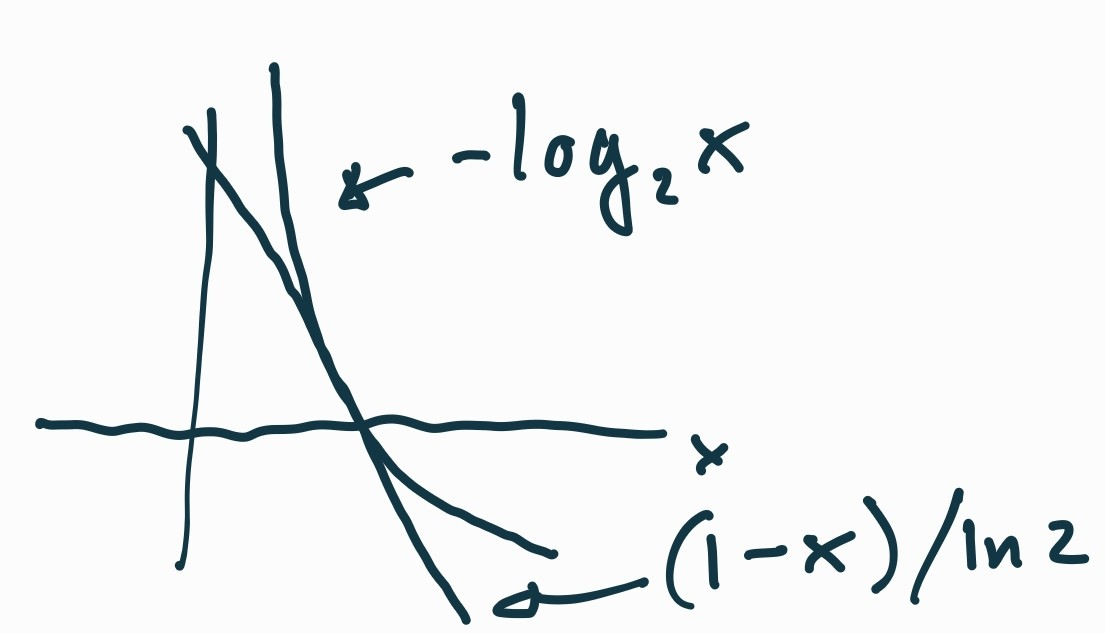
\includegraphics[width=0.5\textwidth]{tempimages/LogBound.jpg}
\end{figure}
	
	To show strict concavity, note that $- \log x \geq \frac{1-x}{\ln 2}$ with the equality holding if and only if $x=1$. We have
	\begin{equation}
		\begin{aligned}
			S(p\rho_1 + \bar{p}\rho_2) &= - \int_X \left(p\rho_1 + \bar{p}\rho_2\right) \log \left(p\rho_1 + \bar{p}\rho_2\right) d\mu \\
			&= - \int_X p\rho_1 \log \left(p\rho_1 + \bar{p}\rho_2\right) d\mu - \int_X \bar{p}\rho_2 \log \left(p\rho_1 + \bar{p}\rho_2\right) d\mu \\
			&= - \int_X p\rho_1 \log \frac{p\rho_1 + \bar{p}\rho_2}{\rho_1} d\mu - \int_X p\rho_1 \log \rho_1 d\mu \\
			&- \int_X \bar{p}\rho_2 \log \frac{p\rho_1 + \bar{p}\rho_2}{\rho_2} d\mu - \int_X \bar{p}\rho_2 \log \rho_2 d\mu \\
			&\geq \int_X p\rho_1 \frac{1}{\ln 2} \left(1 - \frac{p\rho_1 + \bar{p}\rho_2}{\rho_1} \right)   d\mu - p \int_X \rho_1 \log \rho_1 d\mu \\
			&+ \int_X \bar{p}\rho_2 \frac{1}{\ln 2} \left(1 - \frac{p\rho_1 + \bar{p}\rho_2}{\rho_2} \right)   d\mu - \bar{p} \int_X \rho_2 \log \rho_2 d\mu \\
			&= \frac{p}{\ln 2}\left[ \int_X \rho_1 d\mu - \int_X \left(p\rho_1 + \bar{p}\rho_2\right) d\mu  \right] + p S(\rho_1) \\
			&+ \frac{\bar{p}}{\ln 2}\left[ \int_X \rho_2 d\mu - \int_X \left(p\rho_1 + \bar{p}\rho_2\right) d\mu  \right] + \bar{p} S(\rho_2) \\
			&= \frac{p}{\ln 2}\left[ 1 - 1  \right] + p S(\rho_1) + \frac{\bar{p}}{\ln 2}\left[ 1 - 1 \right] + \bar{p} S(\rho_2) \\
			&= p S(\rho_1) + \bar{p} S(\rho_2) \\
		\end{aligned}
	\end{equation}
	The equality holds if and only if $\frac{p\rho_1 + \bar{p}\rho_2}{\rho_1} = 1$ which is exactly when $\rho_1 = \rho_2$.
		
	
\begin{figure}[h]
	\centering
	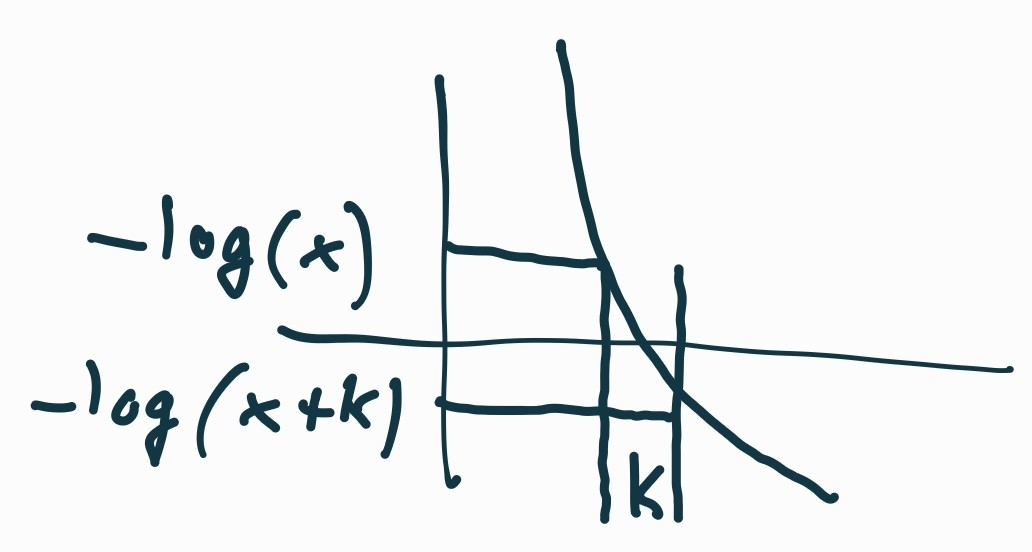
\includegraphics[width=0.5\textwidth]{tempimages/LogMonotone.jpg}
\end{figure}
	For the upper bound, note that the logarithm is a strictly increasing function, and therefore $- \log(x + k) \leq -\log(x)$ for any $k \geq 0$, with equality holding if and only if $k=0$. We have
	\begin{equation}
		\begin{aligned}
			S(p\rho_1 + \bar{p}\rho_2) &= - \int_X \left(p\rho_1 + \bar{p}\rho_2\right) \log \left(p\rho_1 + \bar{p}\rho_2\right) d\mu \\
			&= - \int_X p\rho_1 \log \left(p\rho_1 + \bar{p}\rho_2\right) d\mu - \int_X \bar{p}\rho_2 \log \left(p\rho_1 + \bar{p}\rho_2\right) d\mu \\
			&\leq  - \int_X p\rho_1 \log p\rho_1 d\mu - \int_X \bar{p}\rho_2 \log \bar{p}\rho_2 d\mu\\
			&=  - \int_X p\rho_1 \log p d\mu - \int_X p\rho_1 \log \rho_1 d\mu - \int_X \bar{p}\rho_2 \log \bar{p} d\mu - \int_X \bar{p}\rho_2 \log \rho_2 d\mu\\
			&=  - p \log p \int_X \rho_1 d\mu - p \int_X \rho_1 \log \rho_1 d\mu - \bar{p} \log \bar{p} \int_X \rho_2 d\mu - \bar{p} \int_X \rho_2 \log \rho_2 d\mu\\
			&=  - p \log p - \bar{p} \log \bar{p} + p S(\rho_1) + \bar{p} S(\rho_2)\\
		\end{aligned}
	\end{equation}
	The equality holds if and only if $\rho_2=0$ wherever $\rho_1\neq0$ and $\rho_1=0$ wherever $\rho_2\neq0$. That is, the equality holds if and only if the two distributions have disjoint support. Therefore orthogonal distributions are exactly distributions with disjoint support.
	
	Note that two distributions that have disjoint support have no common components. That is, there is no $\rho_3$ such that $\rho_1 = p \rho_3 + \bar{p} \rho_4$ and $\rho_2 = q \rho_3 + \bar{q} \rho_5$. This is because $\rho_3$ would have to have support that is both within the support of $\rho_1$ and $\rho_2$. Therefore orthogonality implies separateness.
	
	Suppose $\rho_4$ has disjoint support from $\rho_1 = p \rho_2 + \bar{p} \rho_3$, then it has disjoint support from $\rho_2$ and $\rho_3$ because the support of $\rho_1$ is the union of the supports of $\rho_2$ and $\rho_3$. Conversely, if $\rho_4$ has disjoint support from both $\rho_2$ and $\rho_3$, then $\rho_4$ has disjoint support from $\rho_1$ as well. Therefore mixtures preserve orthogonality.
	
	All these arguments are valid for discrete classical ensemble spaces, changing integrals to sums.
	
	For the quantum case, we haven't found a short proof that does not require defining the KL divergence and the entropy for a joint distribution. The result, however, is generally known and can be found, for example, in \href{https://www.cambridge.org/highereducation/books/quantum-computation-and-quantum-information/01E10196D0A682A6AEFFEA52D53BE9AE}{Nielsen-Chuang}.
\end{proof}

\begin{defn}
	Two sets of ensembles are orthogonal if all the elements of one are orthogonal to all the elements of the other. That is, $A \ortho B$ with $A, B \subseteq \Ens$ if $\ens[a] \ortho \ens[b]$ for all $\ens[a] \in A$ and $\ens[b] \in B$. 
\end{defn}

\section{Entropic constraints on the space}

The axioms of entropy not only constrain the functional form of the entropy, but they also constrain the type of space we can have. It also rules out some spaces that would seem physically pathological.

\subsection{Vector space embedding}

The axioms of mixture do not constrain the convex set to be a subset of a vector space. The axioms of entropy, however, do. To be specific, it is the first three properties of the entropy that constrain the space.

\begin{prop}
	A convex space $X$ embeds into a vector space if and only if it is \textbf{cancellative}, that is $p \ens[a] + \bar{p} \ens = p \ens[b] + \bar{p} \ens$ for some $p \in (0,1)$ implies $\ens[a] = \ens[b]$.
\end{prop}

\begin{proof}
	Theorem 4 in \href{https://arxiv.org/abs/1105.1270}{this paper} states that a convex space embeds into a real vector space with $c_\lambda(x,y) = \lambda x + \bar{\lambda}y$ if and only if
	$$ c_\lambda(x,y) = c_\lambda(x,z) \; \forall \lambda \in (0,1) \implies y = z.$$ TODO: the proof should be adapted and carried over.
\end{proof}

\begin{thrm}[Vector space embedding]
	Let $\ens[a], \ens[b], \ens \in \Ens$ such that $p\ens[a] + \bar{p} \ens = p \ens[b] + \bar{p} \ens$ for some $p \in (0,1)$. Then $\ens[a] = \ens[b]$. Therefore any ensemble space embeds into a real vector space.
\end{thrm}

% Reviewed by: Christine

\begin{proof}
	Let $\ens[a], \ens[b], \ens \in \Ens$ such that $p_0\ens[a] + \bar{p}_0 \ens = p_0 \ens[b] + \bar{p}_0 \ens$ for some $p_0 \in (0,1)$.
	
	First, we show that $p\ens[a] + \bar{p} \ens = p \ens[b] + \bar{p} \ens$ for all $p \in (0,p_0]$. In that case, since $0 < \frac{p}{p_0} \leq 1$, we have
	\begin{equation}
		\begin{aligned}
			p \ens[a] + \bar{p} \ens &= \frac{p}{p_0} (p_0 \ens[a] + \bar{p}_0 \ens) + \overline{\left(\frac{p}{p_0}\right)} \ens = \frac{p}{p_0} (p_0 \ens[b] + \bar{p}_0 \ens) + \overline{\left(\frac{p}{p_0}\right)} \ens = p \ens[b] + \bar{p} \ens.
		\end{aligned}
	\end{equation}
	
	Now we show that $p\ens[a] + \bar{p} \ens = p \ens[b] + \bar{p} \ens$ for all $p \in (0,1)$. Since we want to be able to expand multiple times, we want to be able to find a $p$ such that
	\begin{equation}
		p \ens[a] + p \ens[a] + (1-2p) \ens = p \ens[a] + \bar{p} (p_0 \ens[a] + \bar{p}_0 \ens)= p \ens[a] + \bar{p} p_0 \ens[a] + \bar{p} \bar{p}_0 \ens.
	\end{equation}
	The coefficient of the middle term on both sides of the equality, then, has to match. That is, we want $p = \bar{p} p_0$, which means
	\begin{equation}
		\begin{aligned}
			p&=(1-p)p_0=p_0 - p p_0 \\
			p_0 &= p + p p_0 = (1+p_0) p  \\
			p &= \frac{p_0}{1+p_0}
		\end{aligned}
	\end{equation}
	We have
	\begin{equation}
		\begin{aligned}
			2p \ens[a] + \overline{2p} \ens &=  p \ens[a] + p \ens[a] + (1-2p) \ens =  p \ens[a] + \bar{p} (p_0 \ens[a] + \bar{p}_0 \ens) = p \ens[a] + \bar{p} (p_0 \ens[b] + \bar{p}_0 \ens) \\
			&= p \ens[a] + p \ens[b] + (1-2p) \ens = p \ens[b] + p \ens[a] + (1-2p) \ens = p \ens[b] + \bar{p} (p_0 \ens[a] + \bar{p}_0 \ens) \\
			&= p \ens[b] + \bar{p} (p_0 \ens[b] + \bar{p}_0 \ens) = p \ens[b] + p \ens[b] + (1-2p) \ens \\
			&= 2p \ens[b] + \overline{2p} \ens
		\end{aligned}
	\end{equation}
	Note that $2p \geq p_0$. In fact
	\begin{equation}
		\begin{aligned}
			2p &= \frac{2p_0}{1+p_0} \geq p_0  \\
			2 p_0 &\geq (1+p_0) p_0 = p_0 + p_0^2 \\
			p_0 &\geq p_0^2 \\
		\end{aligned}
	\end{equation}
	which is true since $p_0 \in (0,1)$. Since now the relationship holds for $p_1 = \frac{p_0}{1+p_0} > p_0 $, we can repeat the process again and find that it holds for $p_2 = \frac{p_1}{1+p_1} > p_1$ and so on. Therefore, since we can always find a greater mixing coefficient for which the relationship holds, combined with the previous result, $p\ens[a] + \bar{p} \ens = p \ens[b] + \bar{p} \ens$ for all $p \in (0,1)$.
	
	Now we show that if  $p\ens[a] + \bar{p} \ens = p \ens[b] + \bar{p} \ens$ for all $p \in (0,1)$, then we also have $p(\lambda\ens[a] + \bar{\lambda}\ens[b]) + \bar{p} \ens = p\ens[a] + \bar{p} \ens = p \ens[b] + \bar{p} \ens$ for all $\lambda \in [0,1]$. We have
	\begin{equation}
		\begin{aligned}
			p(\lambda\ens[a] + \bar{\lambda}\ens[b]) + \bar{p} \ens &= \lambda(p \ens[a] + \bar{p} \ens) + \bar{\lambda}(p\ens[b] + \bar{p} \ens) = \lambda(p \ens[a] + \bar{p} \ens) + \bar{\lambda}(p\ens[a] + \bar{p} \ens) \\
			&= p\ens[a] + \bar{p} \ens = p\ens[b] + \bar{p} \ens 
		\end{aligned}
	\end{equation}
	
	Lastly, we show that $S(\lambda \ens[a] + \bar{\lambda} \ens[b]) = S(\ens[a]) = S(\ens[b])$ for all $\lambda \in [0,1]$. Using the entropy bounds, with $\lambda \in [0,1]$, we have
	\begin{equation}
		\begin{aligned}
			\lim\limits_{p \to 1} S(p(\lambda\ens[a] + \bar{\lambda}\ens[b]) + \bar{p}\ens) &\leq \lim\limits_{p \to 1} I(p,\bar{p}) + p S(\lambda\ens[a] + \bar{\lambda}\ens[b]) + \bar{p} S(\ens) = S(\lambda\ens[a] + \bar{\lambda}\ens[b]) \\
			\lim\limits_{p \to 1} S(p(\lambda\ens[a] + \bar{\lambda}\ens[b]) + \bar{p}\ens) &\geq \lim\limits_{p \to 1} p S(\lambda\ens[a] + \bar{\lambda}\ens[b]) + \bar{p} S(\ens) = S(\lambda\ens[a] + \bar{\lambda}\ens[b])
		\end{aligned}
	\end{equation}
	and therefore
	\begin{equation}
		\begin{aligned}		
			\lim\limits_{p \to 1} S(p(\lambda\ens[a] + \bar{\lambda}\ens[b]) + \bar{p}\ens) &= S(\lambda\ens[a] + \bar{\lambda}\ens[b]).
		\end{aligned}
	\end{equation}
	Using the above property, we also have
	\begin{equation}
		\begin{aligned}
			S(\lambda\ens[a] + \bar{\lambda}\ens[b]) &= \lim\limits_{p \to 1} S(p(\lambda\ens[a] + \bar{\lambda}\ens[b]) + \bar{p}\ens) = \lim\limits_{p \to 1} S(p \ens[a] +\bar{p} \ens) = S(\ens[a]) \\
			&= \lim\limits_{p \to 1} S(p \ens[b] +\bar{p} \ens) = S(\ens[b]) \\
		\end{aligned}
	\end{equation}
	Since $S(\lambda\ens[a] + \bar{\lambda}\ens[b]) = \lambda S(\lambda\ens[a] + \bar{\lambda}\ens[b]) + \bar{\lambda} S(\lambda\ens[a] + \bar{\lambda}\ens[b]) = \lambda S(\ens[a]) + \bar{\lambda} S(\ens[b])$, $\ens[a] = \ens[b]$ by strict concavity.
\end{proof}

\begin{defn}
	An element $\ens \in \Ens$ can be expressed as an \textbf{affine combination} of ensembles $\ens = \sum_{i=1}^{n} p_i \ens_i$, where $\ens_i \in \Ens$, $p_i \in \mathbb{R}$ and $\sum_{i=1}^{n} p_i = 1$, if the linear combination in the vector space returns an element of $\Ens$.
\end{defn}

\begin{remark}
	In the same way that not all infinite convex combinations yield valid ensembles, not all finite or infinite affine combinations yield valid ensembles.
\end{remark}

\begin{conj}\label{pm_es_ensemblesAreTVS}
	An ensemble space embeds in a topological vector space.
\end{conj}

\begin{remark}
	It is still an open question whether the ambient vector space must be a topological vector space. 
	
	Axioms of ensemble and mixture are not enough to guarantee. See \href{https://math.stackexchange.com/questions/4921905/cancellative-convex-spaces-and-topological-vector-spaces}{this post}. The issue is we have no guarantee of continuity on the inverse (i.e. subtraction, multiplication for a negative number).
	
	As it is shown later, the entropy provides a pseudo-distance, which allows to create open balls. Moreover, the entropy induces a metric tensor, which may induce a suitable topology.
\end{remark}

\subsubsection{Self-mixtures}

%Reviewed by: Christine

As an example of convex spaces that are non-cancellative, and therefore ruled out as ensemble spaces, we consider one in which an ensemble mixed with a different ensemble gives the original ensemble. We show that this can be made to satisfy the axioms of ensemble and mixture, and therefore it is really the axioms of entropy that rule it out.

\begin{example}[Self-mixture]
	Let $\Ens = \{\ens[a], \ens[b]\}$ be a set endowed with the convex structure that satisfies identity, idempotence, commutativity and such that $p \ens[a] + \bar{p} \ens[b]$ equals $\ens[a]$ if $p=1$ and $\ens[b]$ otherwise. Identity, idempotence and commutativity are satisfied by construction. For associativity, note that the final result of multiple mixtures is $\ens[a]$ if and only if all elements of the mixtures are $\ens[a]$. The order does not matter, and therefore associativity is satisfied. Therefore such structure satisfies at least the axioms of mixtures without the requirement of continuity.
	
	For continuity, we need to look at the inverse image under the mixing operation. Note that $+^{-1}(\emptyset) = \emptyset$ and $+^{-1}(\Ens) = [0,1] \times \Ens \times \Ens$. Since $\emptyset$ and $\Ens$ must be in any topology of $\Ens$, the continuity condition is satisfied for these sets. Next, we have  $+^{-1}(\{\ens[a]\}) = [0,1] \times \{\ens[a]\} \times \{\ens[a]\} \cup [1] \times \{\ens[a]\} \times \{\ens[b]\} \cup [0] \times \{\ens[b]\} \times \{\ens[a]\}$. Note that $[0]$ and $[1]$ are not open sets, therefore $\{\ens[a]\}$ cannot be in the topology of $\Ens$ or mixing would not be continuous. Finally, $+^{-1}(\{\ens[b]\}) = [0,1] \times \{\ens[b]\} \times \{\ens[b]\} \cup [0,1) \times \{\ens[a]\} \times \{\ens[b]\} \cup (0,1] \times \{\ens[b]\} \times \{\ens[a]\} = [0,1) \times \Ens \times \{\ens[b]\} \cup (0,1] \times \{\ens[b]\} \times \Ens$. Since $(0,1]$ and $[0,1)$ are open subsets of $[0,1]$, \{$\ens[b]\}$ can be an open set. Since the topology must be $\textsf{T}_0$, we must include at least $\{\ens[b]\}$ and therefore $\mathsf{T}_{\Ens} = \{\emptyset, \{\ens[b]\}, \{\ens[a], \ens[b]\}\}$ is a $\mathsf{T}_0$ second countable topology for which mixing is continuous. This means that the example satisfies both the axioms of ensemble and of mixture.
\end{example}

It is therefore the entropy that rules out this case. If the entropy of the two ensembles is different, it would jump from $S(\ens[a])$ directly to $S(\ens[b])$ for an infinitesimal mixture which violates the upper bound. If $S(\ens[a])$ equals $S(\ens[b])$, the entropy of the mixture of $\ens[a]$ and $\ens[b]$ is also the same, so the two ensembles cannot possibly be different by strict concavity.

\begin{prop}
	Let $\ens[a], \ens[b] \in \Ens$ such that $p\ens[a] + \bar{p} \ens[b] = \ens[b]$ for some $p \in (0,1]$. Then $\ens[a] = \ens[b]$. 
\end{prop}

\begin{proof}
	We have $p\ens[a] + \bar{p} \ens[b] = \ens[b] = p\ens[b] + \bar{p} \ens[b]$ for some $p \in (0,1]$. Therefore $\ens[a] = \ens[b]$.
\end{proof}

\subsubsection{Boundedness of lines}

Another constraint that the entropy imposes is that every affine direction is bounded, even if there are no endpoints. That is, if we take two ensembles, these will identify a line that contains all the affine combinations in the vector space. The elements of that line that are also in the ensemble space are contained in a bounded segment of that line

\begin{figure}[h]
	\centering
	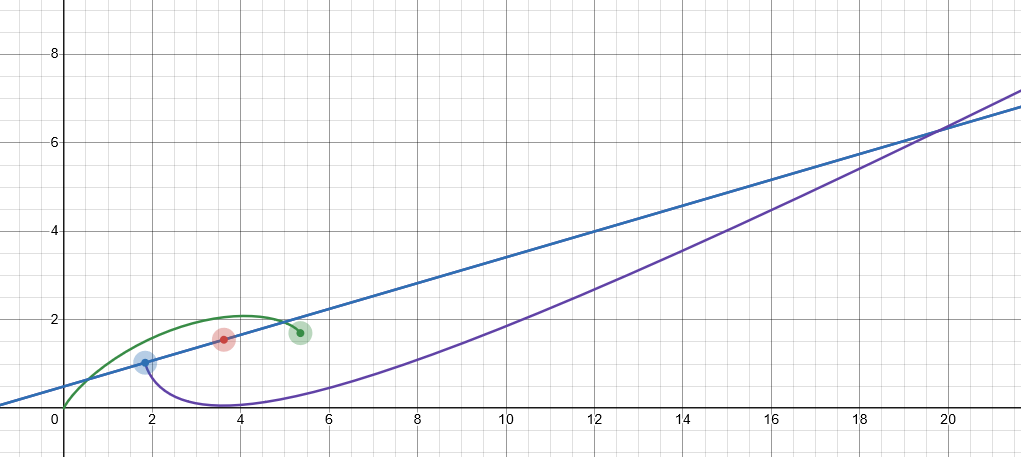
\includegraphics[width=0.9\textwidth]{tempimages/BoundsFromEntropy.png}
	\caption{$\Ens$ is the ensemble space and $V$ is the embedding vector space. Taking to ensembles, the dashed line represents all the affine combinations. Those that are in the ensemble space form a line segment.}
\end{figure}

\begin{defn}
	A \textbf{line} $U \subseteq \Ens$ is a convex subset such that for any three elements one can be expressed as a mixture of the other two. That is, for all $\ens_1, \ens_2, \ens_3 \in U$ there exists a permutation $\sigma$ and $p \in [0,1]$ such that $\ens_{\sigma(1)} = p \ens_{\sigma(2)} + \bar{p} \ens_{\sigma(3)}	$.
\end{defn}

\begin{prop}
	Given $\ens[a], \ens[b] \in \Ens$, there is only one line that contains them.
\end{prop}

\begin{proof}
	Since an ensemble space embeds into a vector space, given two ensembles there is only one affine line that connects them. A line is the intersection of the affine line with the ensemble space.
\end{proof}

\begin{thrm}[Lines are bounded]
	Let $A \subseteq \Ens$ be a line. Then we can find a bounded interval $V \subseteq \mathbb{R}$ and an invertible function $f : A \to V$ such that $f(p \ens[a] + \bar{p} \ens[b]) = p f(\ens[a]) + \bar{p} f(\ens[b])$.
\end{thrm}

\begin{proof}
	Let $A \subseteq \Ens$ be a line. Pick $\ens_0, \ens_1 \in A$. For any $\ens[a] \in A$, we can find a convex expression between $\ens_0$, $\ens_1$ and $\ens[a]$. Rearranging the terms, we can always write $\ens[a] = \bar{x}\ens_0 + x\ens_1$ where $x \in \mathbb{R}$. Note that $x$ is determined and fully determines $\ens[a]$. We can define $f(\ens) \mapsto x$, which will be an invertible function.
	
	We can verify that
	\begin{equation}
		\begin{aligned}
			f(p\ens[a] + \bar{p} \ens[b]) &= f(p\bar{x}_a \ens_0 + px_a \ens_1 + \bar{p}\bar{x}_b \ens_0 + \bar{p}x_b \ens_1) = f((p\bar{x}_a + \bar{p}\bar{x}_b) \ens_0 + (px_a + \bar{p}x_b) \ens_1) \\
			&= px_a + \bar{p}x_b = pf(\ens[a]) + \bar{p}f(\ens[b]).
		\end{aligned}
	\end{equation}
	
	We are going to show that the image $V=f(A)$ must be a bounded set, or it would eventually violate the entropy bounds. Given a value $x \in V$, there will be an entropy value $S(f^{-1}(x))$ which we can write as function of the real value $S(x)$. This function will need to satisfy continuity, strict concavity and upper variability bound.

\begin{figure}[h]
	\centering
	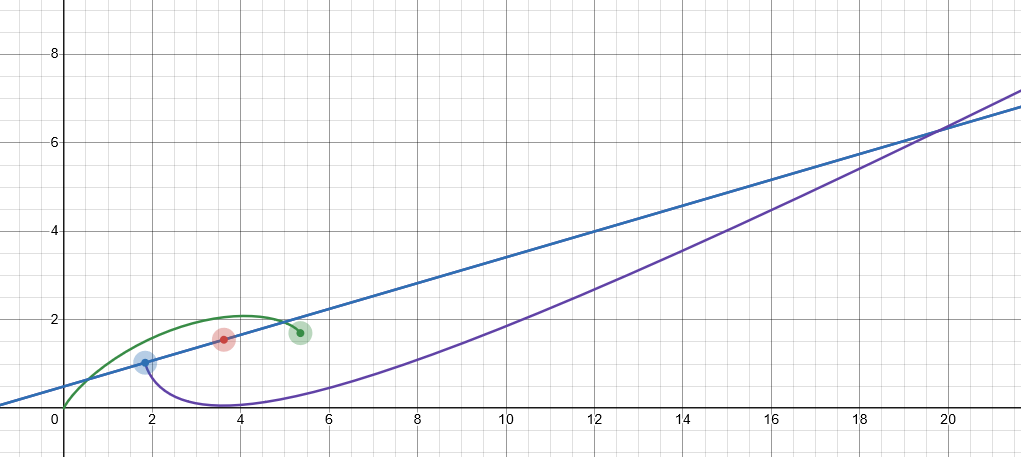
\includegraphics[width=0.7\textwidth]{tempimages/BoundsFromEntropy.png}
\end{figure}
	We are going to show that the function $S(x)$ cannot extend to plus infinity. The same argument can be applied by symmetry for minus infinity. We are going to assume that $S(0) = 0$ without loss of generality. If $S$ is not defined at zero, or if the value is different, we can apply a translation on the argument or on the value, which will not affect the concavity of the function.
	
	Let $0 < a < b \in V$ be two distinct values, with $S(a)$ and $S(b)$ their respective entropies. We are going to show that if pick a $c > b$ sufficiently large, we are not going to find a value for $S(c)$ that satisfies the bounds. In the picture, we have the three points. The blue line is the upper bound on $S(c)$ given by the strict concavity between $a$ and $b$. The purple curve is the lower bound on $S(c)$ given by the upper bound between $0$ and $b$. As the picture shows, the two bounds meet at some point and cannot be satisfied.
	
	From strict concavity, noting that $\frac{c-b}{c-a} + \frac{b-a}{c-a} = 1$, we have:
	\begin{equation}
		\begin{aligned}
			S(b) &= S\left(\frac{c-b}{c-a} a + \frac{b-a}{c-a} c\right) > \frac{c-b}{c-a} S(a) + \frac{b-a}{c-a} S(c)\\
			(b-a)S(c) &< (c-a) S(b) - (c-b) S(a) = (c-a) S(b) - (c-a) S(a) + (b-a) S(a) \\
			S(c) &< \frac{S(b) - S(a)}{(b-a)} (c-a) + S(a) \\
		\end{aligned}
	\end{equation}
	
	From the upper bound, noting that $\frac{c-a}{c} + \frac{a}{c} = 1$, we have:
	\begin{equation}
		\begin{aligned}
			S(a) &= S\left(\frac{c-a}{c} 0 + \frac{a}{c} c\right) \leq I\left(\frac{c-a}{c}, \frac{a}{c}\right) + \frac{c-a}{c} S(0) +\frac{a}{c} S(c) \\
			\frac{a}{c} S(c) &\geq S(a) - I\left(\frac{c-a}{c}, \frac{a}{c}\right) \\
			S(c) &\geq \frac{c}{a} \left[ S(a) - I\left(\frac{c-a}{c}, \frac{a}{c}\right) \right]
		\end{aligned}
	\end{equation}
	
	Combining the bounds, we have:
	\begin{equation}
		\begin{aligned}
			\frac{S(b) - S(a)}{(b-a)} (c-a) + S(a) &> \frac{c}{a} \left[ S(a) - I\left(\frac{c-a}{c}, \frac{a}{c}\right) \right] \\
			(c-a) S(b) - (c-a)S(a) + (b-a) S(a) &> \frac{c(b-a)}{a} S(a) - \frac{c(b-a)}{a} I\left(\frac{c-a}{c}, \frac{a}{c}\right) \\
			a (c-a) S(b) - a(c-b) S(a) &> c(b-a)S(a) - c(b-a) I\left(\frac{c-a}{c}, \frac{a}{c}\right) \\
			a (c-a) S(b) + (-ac +ab -bc +ac) S(a) &> - c(b-a) I\left(\frac{c-a}{c}, \frac{a}{c}\right) \\
			a (c-a) S(b) -b (c-a) S(a) &> - c(b-a) I\left(\frac{c-a}{c}, \frac{a}{c}\right) \\
			a  S(b) - b S(a) &> - \frac{c(b-a)}{(c-a)} I\left(\frac{c-a}{c}, \frac{a}{c}\right) \\
		\end{aligned}
	\end{equation}
	
	Since $b > a$, $c > a$ and $I(p,\bar{p}) \geq 0$ for all $p$, the right hand side of the inequality is always negative. As $c$ increases, the right hand side will go to zero, since $\lim\limits_{c\to \infty}\frac{c(b-a)}{c-a} = b-a$ and $\lim\limits_{c\to \infty} I\left(\frac{c-a}{c}, \frac{a}{c}\right) = I(1,0) = 0$. The left hand side is a constant. If the constant is positive, the inequality is always satisfied. If it is negative, it will not be satisfied for all $c$.
	
	From strict concavity, noting that $\frac{b-a}{b} + \frac{a}{b} = 1$, we have
	\begin{equation}
		\begin{aligned}
			S(a) &= S\left(\frac{b-a}{b} 0 + \frac{a}{b} b\right) > \frac{b-a}{b} S(0) + \frac{a}{b} S(b) = \frac{a}{b} S(b)\\
			b S(a) &> a S(b)  \\
			0 &> a S(b) - b S(a)\\
		\end{aligned}
	\end{equation}
	This shows that the left hand side of the previous inequality is negative, and therefore the bounds cannot be satisfied over the whole $\mathbb{R}$.
	
	This means that $V = f(A)$ must be bounded and therefore every line is a segment as embedded in the vector space
\end{proof}

\begin{remark}
	Note that this does not mean that, along each direction, the line is closed in the vector space. That is, it may not include extreme point in the convex space. An open bounded interval, in fact, it is till a convex space and we would be able to define an entropy on it.
\end{remark}


\section{Generalized probability theory}

\subsection{Fraction and fraction capacity}

%DONE: subsection reviewed by Sharif and Christine

In this section we are going to define \textbf{fraction capacity}, which is a generalization of probability to the non-additive case. The typical way to understand probability is through outcomes of a process: $50\%$ probability for tails means that if we repeated the coin toss multiple times, we would expect roughly half to be tails. In classical mechanics, it can also be understood as the probability of preparation: roughly half the times we selected a preparation procedure that prepared tails. In quantum mechanics, this does not work as the probability used during the mixing is the same as the probability of the outcome only if we are mixing orthogonal states. Effectively, probability in the usual sense is defined only on outcomes. The fraction capacity, instead, defines a measure on preparations.

The fraction capacity tells us how much of an ensemble $\ens$ can be constructed through a mixture of ensembles from a set $A$. It is a non-negative, unit bounded, sub-additive, monotone continuous measure, and it reduces to the probability measure in the classical case, and over measurements in the quantum case. The goal is to create a measure theoretic generalization of probability theory that can work on all ensemble spaces.

First we define the \textbf{fraction} of one element within another. For example, suppose $\ens$ is a uniform distribution for a six-faced die. Suppose $\ens[a]$ represents the outcome 3 with $100\%$ probability. Then $\ens$ can be understood as $\ens = \frac{1}{6} \ens[a] + \frac{5}{6} \ens[b]$ where $\ens[b]$ is the uniform distribution over the outcomes 1,2,4,5 and 6. Note that $\frac{1}{6}$ is the highest coefficient we can put in front of $\ens[a]$ in a convex combination and have $\ens$ as a result, which coincides with the probability of obtaining 3 from a uniform distribution over six outcomes. That is what we define the fraction of $\ens[a]$ in $\ens$ to be.

%TODO picture of the two distributions

\begin{mathSection}
	\begin{defn}
		Let $\ens, \ens[a] \in \Ens$ be two ensembles. The \textbf{fraction} of $\ens[a]$ in $\ens$ is the greatest mixing coefficient for which $\ens$ can be expressed as a mixture of $\ens[a]$. That is, $\size_{\ens}(\ens[a]) = \sup(\{ p \in [0,1] \, | \, \exists \, \ens[b] \in \Ens \text{ s.t. }  \ens = p \ens[a] + \bar{p} \ens[b] \})$.
	\end{defn}
	
	\begin{remark}
		We need to take the supremum as the maximum may not exist. For example, consider a discrete classical ensemble space and remove the endpoints. At the moment, there is no reason to rule out such space as unphysical.
	\end{remark}
	
	\begin{coro}
		Let $\ens, \ens[a] \in \Ens$, then $\size_{\ens}(\ens[a]) = 0$ if and only if $\ens[a]$ is not a component of $\ens$.
	\end{coro}
	
	\begin{proof}
		Note that $\ens[a]$ is a component of $\ens$ if we can write $\ens = \lambda \ens[a] + \bar{\lambda} \ens[b]$ for some $\lambda \in (0,1]$ and $\ens[b] \in \Ens$. In this case, $\size_{\ens}(\ens[a]) \geq \lambda > 0$. Conversely, if $\size_{\ens}(\ens[a]) > 0$ we can find $\size_{\ens}(\ens[a]) \geq \lambda > 0$ such that $\ens = \lambda \ens[a] + \bar{\lambda} \ens[b]$ for some $\ens[b] \in \Ens$.
	\end{proof}
\end{mathSection}

We now define \textbf{fraction capacity} of a set of ensembles for another ensemble. Like before, suppose $\ens$ is a uniform distribution for a six-faced die, but now take $A = \{ \ens[a], \ens[b] \}$ as, respectively, the outcomes $3$ and $4$ with $100\%$ probability. Then $\ens$ can be understood as $\ens = \frac{1}{3} \left(\frac{1}{2} \ens[a] + \frac{1}{2} \ens[b] \right) + \frac{2}{3} \ens[c]$, where $\ens[c]$ is the uniform distribution over outcomes 1,2,5 and 6. Again, note that $\frac{1}{3}$ is the highest coefficient we can put in front of any convex combinations of elements of $A$, and still make a convex combination that has $\ens$ as a result. That is what we define the fraction capacity of $A$ for $\ens$ to be.

The fraction capacity, then, defines how much of the ensemble $\ens$ can be constructed with elements of $A$. The term capacity is used first because, intuitively, it tells us how much $A$ can hold, and second because capacity is a name used to describe non-additive measures. The fraction capacity, in fact, is shown to have several nice properties. First, its value is always between zero and one, since the coefficient of a convex combination must be so bound. Second, it is monotone in the sense that if $A$ gets bigger, the fraction capacity cannot decrease. Third, it is subadditive, meaning that the fraction capacity of the union of two sets must be the sum of the respective fraction capacities or less. Fourth, it is continuous. Note that if subadditivity is replaced by additivity, these are exactly the defining properties of a probability measure, since additivity and continuity are equivalent to $\sigma$-additivity.

\begin{mathSection}
	\begin{defn}
		Let $\ens \in \Ens$ be an ensemble and $A \subseteq \Ens$ a Borel set. The \textbf{fraction capacity} of $A$ for $\ens$ is the biggest fraction achievable with convex combinations of $A$. That is, $\fcap_{\ens}(A) = \sup(\size_{\ens}(\hull(A))\cup\{0\})$.
	\end{defn}
	
	\begin{coro}
		The fraction capacity uniquely identifies an ensemble. That is, let $\ens[a], \ens[b] \in \Ens$ such that $\ens[a] \neq \ens[b]$. Then $\fcap_{\ens[a]} \neq \fcap_{\ens[b]}$.
	\end{coro}
	
	\begin{proof}
		Note that $\ens = 1 \ens[a] + 0 \ens[b]$ if and only if $\ens = \ens[a]$. Therefore, let $\ens[a], \ens[b] \in \Ens$ such that $\ens[a] \neq \ens[b]$. We have $\fcap_{\ens[a]}(\{\ens[a]\}) = 1$ and $\fcap_{\ens[b]}(\{\ens[a]\}) \neq 1$. Which means $\fcap_{\ens[a]} \neq \fcap_{\ens[b]}$.
	\end{proof}
	
	\begin{prop}
		The fraction capacity for an ensemble is a set function that is
		\begin{enumerate}
			\item non negative and unit bounded: $\fcap_{\ens}(A) \in [0,1]$
			\item monotone: $A \subseteq B \implies \fcap_{\ens}(A) \leq \fcap_{\ens}(B)$
			\item subadditive: $\fcap_{\ens}(A \cup B) \leq \fcap_{\ens}(A) + \fcap_{\ens}(B)$
			\item continuous from below: $\fcap_{\ens}(\lim\limits_{i \to \infty} A_i) = \lim\limits_{i \to \infty} \fcap_{\ens}(A_i)$ for any increasing sequence $\{A_i\}$
			\item continuous from above: $\fcap_{\ens}(\lim\limits_{i \to \infty} A_i) = \lim\limits_{i \to \infty} \fcap_{\ens}(A_i)$ for any decreasing sequence $\{A_i\}$
		\end{enumerate}
	\end{prop}
	
	\begin{proof}
		1. The fraction capacity takes a subset of $\Ens$ and returns a real value and is therefore a set function. The mixture coefficients are real values between zero and one. The supremum of a set of numbers between zero and one is between zero and one, and therefore the fraction capacity for an ensemble is non negative and unit bounded.
		
		2. The $\hull$ is a monotone function. The image of a set through a map is a monotone function. The supremum is a monotone function. Therefore the fraction capacity is a monotone function.
		
		3. Let $A, B \subseteq \Ens$ and let $p \in [0,1]$ such that $\ens = p \ens_1 + \bar{p} \ens_2$ for some $\ens_1 \in \hull(A \cup B)$ and $\ens_2 \in \Ens$. Since $\ens_1 \in \hull(A \cup B)$, we can write $\ens_1 = \lambda \ens[a] + \bar{\lambda} \ens[b]$ for some $\lambda \in [0,1]$, $\ens[a] \in A$ and $\ens[b] \in B$. Therefore we have $\ens = p \lambda \ens[a] + p \bar{\lambda} \ens[b] + \bar{p} \ens_2$. By the definition of fraction capacity, we must have $p\lambda \leq \fcap_{\ens}(A)$ and $p\bar{\lambda} \leq \fcap_{\ens}(B)$, therefore $p = p\lambda + p\bar{\lambda} \leq \fcap_{\ens}(A) + \fcap_{\ens}(B)$. 	Since $\fcap_{\ens}(A \cup B)$ is the supremum for a set of $p$s for which the expression always holds, we have $\fcap_{\ens}(A \cup B) \leq \fcap_{\ens}(A) + \fcap_{\ens}(B)$. The fraction capacity is subadditive.
		
		4. Let $\{A_i\} \subseteq \Sigma_{\Ens}$ be an increasing sequence. That is $A_i \subseteq A_{i+1}$ for all $i$. Given that the fraction capacity is monotone, $\{\fcap_{\ens}(A_i)\}$ is an increasing sequence. Note that $\fcap_{\ens}(A_i) \leq 1$ for all $i$, therefore the sequence will have an upper bound which will coincide with the limit. Let $A = \lim\limits_{i \to \infty} A_i$. We have $A = \bigcup A_i$ and $A_i \subseteq A$ for all $i$. Since fraction capacity is monotone, we have $\fcap_{\ens}(A_i) \leq \fcap_{\ens}(A)$ for all $i$ and therefore $\lim\limits_{i \to \infty} \fcap_{\ens}(A_i) \leq \fcap_{\ens}(A)$. Suppose $\lim\limits_{i \to \infty} \fcap_{\ens}(A_i) < \fcap_{\ens}(A)$. Then there would be an $\ens[a] \in \hull(A)$ such that $\size_{\ens}(\ens[a]) > \size_{\ens}(\ens[b])$ for all $\ens[b] \in \hull(A_i)$ for all $i$. But if $\ens[a] \in \hull(A)$, then it is a convex combination of finitely many elements of $A$. Given that $\{A_i\}$ is an increasing sequence, there will be a $A_k$ that will contain those finitely many elements, and therefore $\ens[a] \in \hull(A_k)$ which is a contradiction. Therefore $\lim\limits_{i \to \infty} \fcap_{\ens}(A_i) = \fcap_{\ens}(A)$.
		
		5. The previous argument works in the same way for decreasing sequences.
	\end{proof}
\end{mathSection}

\begin{conj}
	The fraction capacity is $\sigma$-subadditive. That is, $\fcap_{\ens}(\bigcup A_i) \leq \sum \fcap_{\ens}(A_i)$.
\end{conj}

\begin{remark}
	In \href{https://link.springer.com/book/10.1007/978-3-319-30690-2}{Set Functions, Games and Capacities in Decision Making}, it is claimed that finite additivity plus continuity implies $\sigma$-additivity. The conjecture is that this generalizes to $\sigma$-subadditivity.
\end{remark}


\subsection{Maximal component sequence}

\begin{defn}
	Let $\ens \in \Ens$ be an ensemble. A sequence of ensembles $\{\ens[a]_i\} \subseteq \Ens$ is an \textbf{increasing component sequence of $\ens$} if we can write
	\begin{align*}
		\ens &= p_i \ens[a]_i + \bar{p}_i \ens[b]_i  \\
		\ens[a]_{i+1} &= \frac{p_i}{p_{i+1}} \ens[a]_i + \frac{p_{i+1} - p_i}{p_{i+1}} \Delta \ens[a]_i
	\end{align*}
	where $\{\ens[b]_i\} \subseteq \Ens$, $\{\Delta\ens[a]_i\} \subseteq \Ens$ and $\{p_i\} \subseteq (0,1]$ is an increasing sequence. The \textbf{fraction} of the sequence is the limit $p_i \to p$.
\end{defn}

\begin{remark}
	Since the sequence of $p_i$ is increasing and is bounded, it must converge. The set of all possible limits is bounded and therefore must have a supremum.
\end{remark}

\begin{defn}
	Let $\ens \in \Ens$ be an ensemble and $A \subseteq \Ens$ a set of ensembles. Then the \textbf{$A$-components of $\ens$} are the components of $\ens$ that are mixtures of $A$. That is, $A_{\ens} = \{ \ens_1 \in \hull(A) \, | \, \exists p \in (0,1], \ens_2 \in \Ens \text{ s.t. } \ens = p \ens_1 + \bar{p} \ens_2  \}$. An \textbf{increasing $A$-component sequence of $\ens$} is an increasing component sequence of $\ens$ such that $\{\ens[a]_i\} \subseteq \hull(A)$ and $\{\Delta\ens[a]_i\} \subseteq \hull(A)$. The sequence $\{\ens[a]_i\} \subseteq \hull(A)$ is \textbf{maximal} if the fraction of the sequence is $\fcap_{\ens}(A)$.
\end{defn}

\begin{coro}
	The fraction of $A$-component sequences are bounded by $\fcap_{\ens}(A)$.
\end{coro}

\begin{proof}
	For all elements of component sequences we have $p_i \leq \fcap_{\ens}(A)$. Therefore the limit of $p_i$ cannot exceed $\fcap_{\ens}(A)$.
\end{proof}

\begin{prop}
	Let $\ens \in \Ens$ be an ensemble and $A \subseteq \Ens$ a set of ensembles, then there exists a maximal $A$-component sequence of $\ens$.
\end{prop}

\begin{proof}
	Consider the hull of $A$. This can be ordered by the fraction $\size_{\ens}$, which is less or equal to one. If there is a maximum, then simply take a sequence of an element with the maximum faction. If not, we can take a sequence of ever increasing fractions whose limit is the fraction capacity, and find a corresponding sequence of ensembles within $\hull(A)$. By definition, this will be a maximal $A$-component sequence of $\ens$.
\end{proof}

\begin{prop}
	Let $\{\ens[a]_i\} \subseteq \hull(A)$ be an $A$-component sequence of $\ens \in \Ens$. A \textbf{complement} sequence is an increasing sequence $\{\ens[b]_i\} \subseteq \Ens$ such that
	$$ \ens = p_i \ens[a]_i + q_i \ens[b]_i + \overline{(p_i + q_i)} \ens[\epsilon]_i $$
	where $\{\ens[\epsilon]_i\} \in \Ens$ and $(p_i + q_i) \to 1$. In this sense, the sum of the two sequences converges to $\ens$.
\end{prop}

\begin{remark}
	Note that complement sequences always exist since we can set $\ens[\epsilon]_i = \ens[b]_i$, $q_i = \bar{p}$ and recover the definition of a component sequence.
\end{remark}

\begin{prop}
	An $A$-component sequence $\{\ens[a]_i\} \subseteq \hull(A)$ of $\ens \in \Ens$ is maximal if and only if it admits a complement sequence that is always separate from the hull of A. That is, $\{\ens[b]_i\} \separate \hull(A)$.
\end{prop}

\begin{proof}
	Suppose that $\{\ens[a]_i\}$ is maximal and let $\{\ens[b]_i\}$ be a complement.
	$$ \ens = p_i \ens[a]_i + q_i \ens[b]_i + \overline{(p_i + q_i)} \ens[\epsilon]_i.$$
	
\end{proof}

\begin{prop}
	Let $\ens \in \Ens$ be an ensemble, $A \subseteq \Ens$ a set of ensembles and $\ens[a]_i$ and $\ens[b]_i$ two maximal $A$-component sequence of $\ens$. Then we can write $\ens[a]_i = p_i \ens[b]_i + \bar{p}_i \ens[c]_i$ where $\ens[c]_i \in \Ens$, $p_i \in [0,1]$ and $p_i \to 1$.
\end{prop}

\begin{proof}
	Note that we can always write $\ens[a]_i = p_i \ens[b]_i + \bar{p}_i \ens[c]_i$ because we can always choose $p_i = 0$ and $\ens[c]_i = \ens[a]_i$. Therefore, if the proposition is not true, we can always find $p_i \to p$, except that $p \neq 1$.
	
	Suppose the proposition is not true. We can still write $\ens = \lambda_i \ens[a]_i + \bar{\lambda}_i \ens[d]_i = \lambda_i p_i \ens[b]_i + \lambda_i \bar{p}_i \ens[c]_i + \bar{\lambda}_i \ens[d]_i$. But $\ens[b]_i$ is maximal, therefore $\lambda_i p_i \ens[b]_i$ can be increased. But $\ens[c]_i \in \hull(A)$, which means we can write an $A$-component sequence whose fraction is higher than the maximal, which cannot be. Therefore the proposition is true.
	
	TODO: this may need to be fixed. Can't reconstruct the argument.
\end{proof}

\subsection{Classical probability contexts}

In this section we are going to define what classical probability contexts are and give a set of necessary and sufficient conditions for ensemble spaces, or subsets of ensemble spaces, to form a classical probability context. That is, for the ensembles to be represented using the standard tools of classical probability.

We want a simple definition that captures the intuition of spaces of classical probability distributions in a way that works well for infinite dimensional spaces, is compatible with both discrete and continuous classical ensemble spaces but also with measurements context in quantum ensemble spaces. It is instructive to go through some of the different attempts to understand why we settled on these definitions, so that one can understand why they work.

The first idea would be to define a classical probability context as the set of all probability measures over a space $X$. This is too broad as it includes probability measures that are unphysical. If $X$ is a countable discrete space, some probability measure will have infinite entropy. If $X$ is a real line, a probability measure concentrated at a point (i.e. a discrete measure) would have minus infinite entropy. There are two distinct problems here, let us look at them closely one at a time.

The first problem is due to the spread of a finite amount of probability over an infinite region. This problem is strictly connected to characterizing what is the correct closure under infinite convex combination. Since we want the topology to determine which infinite convex combinations are allowed, we want a notion of classical probability context that guarantees the closure only on finite convex combinations and lets the closure in the topology extend sets to infinite convex combinations. Therefore, the solution here is to let topological structure handle this problem, and assume that different spaces will have, potentially, different closures.

The second problem is due to the spread of a finite amount of probability over a measure zero set. In classical mechanics, requiring a probability measure to be absolutely continuous with respect to the Liouville measure avoids the problem. Recall that a measure $p$ is \href{https://en.wikipedia.org/wiki/Absolute_continuity#Absolute_continuity_of_measures}{absolutely continuous} with respect to $\mu$ if $\mu(U) = $ implies that $p(U)=0$. That is, the probability is zero over any set for which the Liouville measure is zero. Physically, if the set contains zero states, it has zero probability. Note that the Liouville measure is connected to the entropy and, as we will see later, to the state capacity. However, this solution is not general enough, as there are cases in which we will want a probability defined at a point over the continuum. For example, we are able to prepare a mixture of water, water vapor and ice in thermodynamic equilibrium. This would correspond to a point in the pressure/volume diagram. Therefore, we can create a distribution with finite probability over few, very special points. What we need is a compatibility condition between each measures and the topology of the space, instead of across measures. Note that this is the topology of the space that supports the measure (i.e. phase space in classical mechanics) not the topology of the ensemble space (i.e. the space of probability distributions over phase space in classical mechanics). Therefore we will also need to relate the topology of the space that supports the measures with the ensemble space it represents.

Recall that an open set corresponds to an experimentally verifiable statement. Imagine we prepared a distribution over some variable, and have a test that tells us whether the value of an instance is within a specific range $U$. Then the open set $U$ corresponds to the positive outcome of the test. The exterior $\exterior(U)$ corresponds to cases we are able to tell apart from those from $U$ with another test, one that fails if the instance is in $U$. The boundary $\partial U$ corresponds to those cases we are not be able to adjudicate experimentally: they are not in $U$, but are too close to $U$ to discern from $U$. That is, there is no test that can tell us we have an element of $\partial U$, these cases are not detectable. Assigning a non-zero probability or count of states to these sets, then, would be physically unjustifiable. Therefore, a measure of probability should assign non-zero values directly only to open sets, and the closure of open sets should have the same probability. We have therefore a physically justifiable assignment on both open sets and closed sets. The collection of open and closed sets forms a ring, in the sense that it is closed under complement and finite union. \href{https://en.wikipedia.org/wiki/Carath%C3%A9odory's_extension_theorem}{Carath\'{e}odory's extension theorem} guarantees a unique extension to the whole Borel algebra. For a measure that counts configurations we will additionally require that every open set correspond to a non-zero number of configurations. This means that a probability measure will necessarily be absolutely continuous with respect to the count of configurations, and therefore a probability density will always be well defined. In this section, we will only concentrate on the probability measure and its compatibility with the topology.

To sum up, given a topological space $X$, we are interested in measures that are topologically compatible, in the sense that $p(U) = p(\bar{U})$ for every open set $U$. We stress that this is not necessarily true for any Borel set, just for open sets. Consider, in fact, the set of rationals $\mathbb{Q}$ as a subset of the reals $\mathbb{R}$. This is a measure zero subset whose closure is the whole space. Therefore, if $p$ is a probability measure over the reals, we would have $p(\mathbb{R}) = p(\overline{\mathbb{Q}}) = p(\mathbb{Q})$ which would mean that the probability is all concentrated on a set of measure zero, which is exactly what we do not want. The requirement, then, holds only for open sets. Conversely, it is not true that all sets of measure zero are boundaries of open sets. The set of rationals is not the boundary of an open set.

Having somewhat clarified what a ``well-behaved'' probability distribution looks like, by requiring its compatibility to the topology, we now want to understand what subsets of an ensemble space can be understood as a classical probability context. Roughly speaking, we want to be able to think of a classical probability context as the set of all the ``well-behaved'' probability distributions over a set of cases. We have to clarify what do we mean by ``all.'' Requiring the set of probability measures to be closed under convex combinations does not seem to be not enough. The cut triangle \ref{pm_es_cutTriangle}, for example, is a subset of a set of discrete classical ensemble space where not all ensembles can be understood as a unique convex combination of the extreme points, precisely because some cases are missing. This convex subset is leaving out some ensembles, making a classical space not look classical. On the other hand, if we take a Bloch ball, we can take three points on the surface. These would form a triangle, which could be understood as a discrete classical probability space. Here the convex closure is leaving out some ensembles, making a non-classical space look classical. Therefore we have two problem: what is the correct closure we should be looking at? How can we formulate the classical property?

As an early attempt, we though extending the closure to both mixtures and components. That is, closure on the convex structure would require $\ens[a] = p \ens[b] + \bar{p} \ens[c]$ to be in the set if both $\ens[b]$ and $\ens[c]$. Closure on the components would also require $\ens[b]$ and $\ens[c]$ to be in the set if $\ens[a]$ is present. This seems to take too much in. In quantum mechanics, for example, a single mixed state would bring in all the mixed states in the smallest subspace that contains it.

The correct closure seems to be to include all affine combinations. That is, if $\ens[a] = p \ens[b] + \bar{p} \ens[c]$ and two of the ensembles are in the set, then the other one is in the set as well. This allows us to get all the ensembles in the same hyperplane. We call this a flat. In the triangle example, the only flats available are the single vertexes, each side and the whole triangle. For the Bloch ball, if we took two elements, we would get the whole segment that connects them and extends to the surface. But if we get three points, we get a circle, which is not a simplex. A classical probability context, then, is a flat where we can guarantee single decomposition: they are simplexes. While this needs to be stated carefully, so that it can work in infinite dimensions, this is the core idea.

% Reviewed with Christine start

\begin{defn}
	A \textbf{simplex} is a subset $U \subset \mathbb{R}^n$ that is the hull of finitely many affinely independent points. That is, $U = \hull(\{x_i\}_{i=0}^{n})$ such that $\{x_i - x_0\}_{i=1}^{n}$ are linearly independent.
\end{defn}

\begin{defn}
	A \textbf{flat} $A \subseteq \Ens$ is a closed convex subset that contains all lines between all elements. That is, for any $\ens[a], \ens[b] \in A$, $A$ also contains the line that contains $\ens[a]$ and $\ens[b]$. Given a set $U \subseteq \Ens$, the \textbf{flat closure} of $U$ is the smallest flat that contains $U$. A flat is \textbf{finite} if it can be generated by a finite number of elements. An $n$-flat is a flat that must be generated by a set with at least $n$ elements.
\end{defn}

\begin{figure}[h]
	\centering
	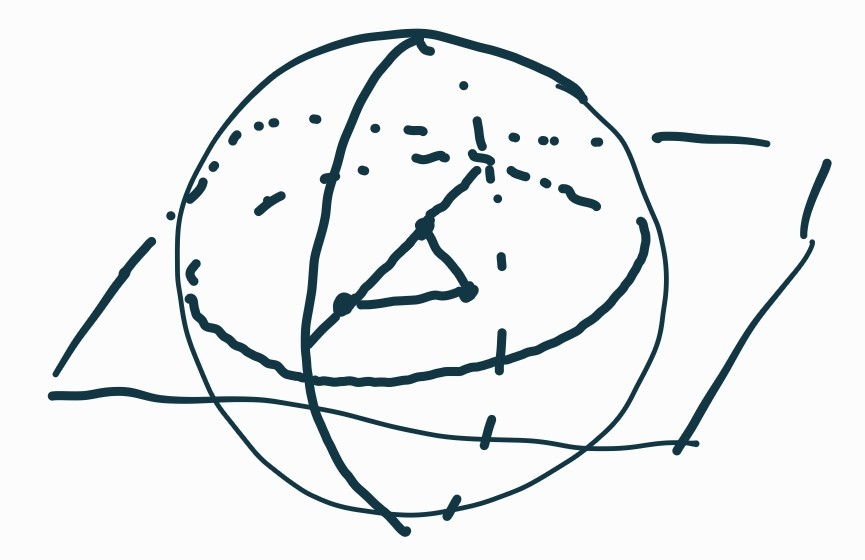
\includegraphics[width=0.4\textwidth]{tempimages/FlatVsConvex.jpg}
	\caption{Flat vs convex set. The ball is the ensemble space. The triangle represents a convex subset. The disc containing the triangle is the flat closure of the triangle. The plane is the affine closure of the triangle.}
\end{figure}


\begin{prop}
	A flat includes all possible affine combinations of elements of $\Ens$ that are contained in $\Ens$. The flat closure of $U \subseteq \Ens$ is the intersection of $\Ens$ with the affine closure of $U$ in the embedding vector space.
\end{prop}

\begin{proof}
	Let $A \subseteq \Ens$ be a flat and let $V$ be the real vector space that embeds $\Ens$. A line between two elements $\ens[a], \ens[b] \in A$ can be extended in $V$ and can be written as $\ens[a] + x \left(\ens[b] - \ens[a]\right)$ with $x \in \mathbb{R}$. Therefore any ensemble that can be written as an affine combination of two ensembles in $A$ is an element of the flat. Recursively, this means that any ensemble that can be written as an affine combination of finitely many ensembles in $A$ is also in the flat. Moreover, since the flat is a closed set, it will also include all its limits. Therefore every affine combination of $A$ that is also an element of $\Ens$ is in $A$, which means $A$ is the intersection of an affine subspace of the embedding vector space and the ensemble space.
	
	Now let $U \subseteq \Ens$ be a set of ensembles. The affine closure of $U$ will be an affine subspace of the embedding vector space. The flat closure will be the intersection of the affine closure with $\Ens$. Since the affine closure is the smallest closed affine subspace that contains $U$, its intersection with $\Ens$ will be the smallest flat that contains $U$, which is the flat closure of $U$.
\end{proof}

\begin{conj}
	An $n$-flat is a simplex if and only if its $3$-flats are simplexes (i.e. triangles).
\end{conj}

\begin{remark}
	In classical discrete ensemble spaces, any flat is a simplex. In classical continuous ensemble spaces, infinite dimensional flats will depend on what limits are allowed. In a quantum ensemble space, if we take three ensembles inside a Bloch ball, the corresponding flat will be a circle. If we take three orthogonal pure states, however, the corresponding flat will be a simplex.
\end{remark}

\begin{defn}
	An ensemble is \textbf{decomposable} if it can be expressed as a mixture of two ensembles. An ensemble is \textbf{separately/orthogonally decomposable} if it can be expressed as a mixture of two separate/orthogonal ensembles. An ensemble is \textbf{separately multidecomposable} if it can be expressed as two decompositions where a component of one is separate from both components of the other. That is, $\ens = p \ens[a]_1 + \bar{p} \ens[a]_2 = \lambda \ens[b]_1 +\bar{\lambda} \ens[b]_2$ and either $\ens[a]_1 \separate \ens[b]_j$ or $\ens[a]_2 \separate \ens[b]_j$.
\end{defn}

\begin{figure}[h]
	\centering
	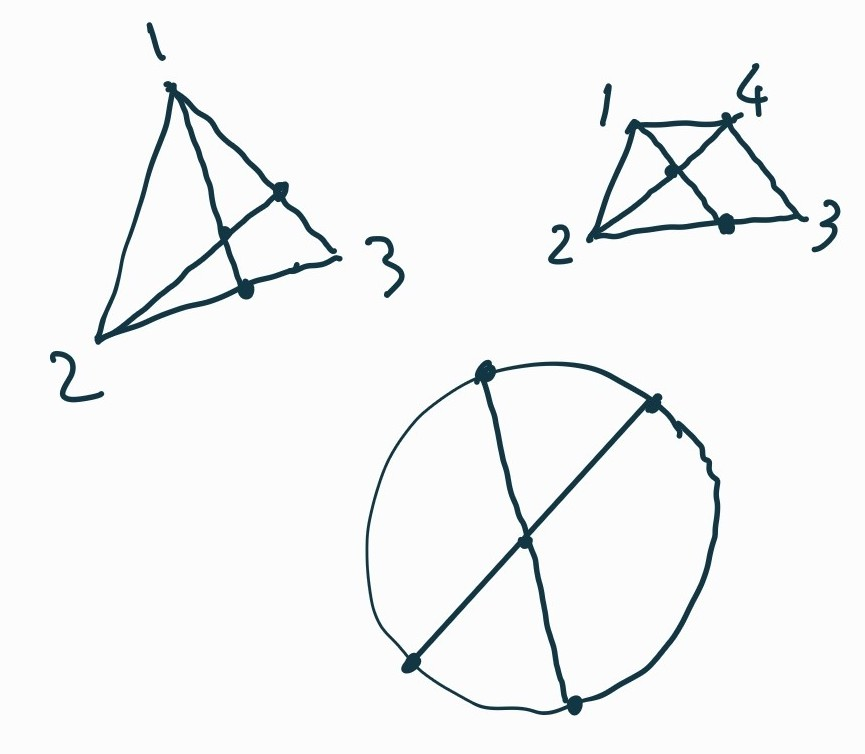
\includegraphics[width=0.4\textwidth]{tempimages/MultipleDecomposition.jpg}
\end{figure}

\begin{remark}
	Take a classical discrete space for three points which is a triangle (simplex). The only three elements that are not decomposable are the extreme points. Mixtures of two points are decomposable and are also separately decomposable in only one way. Mixtures of three points are also separately decomposable, but in multiple ways: as a mixture of $\ens_1$ and a mixture of $\ens_2$ and $\ens_3$, or as a mixture of $\ens_2$ and a mixture of $\ens_1$ and $\ens_3$. Note, however, that they are not separately multidecomposable as the different components are not separate.
	
	Take a Bloch ball for quantum mechanics. All the elements of the surface are not decomposable and they are all pairwise separate. The middle point can be seen as the equal mixture of any pair of opposite points. Therefore the middle point, as well as any other point not on the surface, is not only separately decomposable but also multidecomposable.
	
	To see why we require only one component to be separate from the other two, consider the cut triangle. Here we can have multiple decompositions where not all elements are separate.
\end{remark}

\begin{figure}[h]
	\centering
	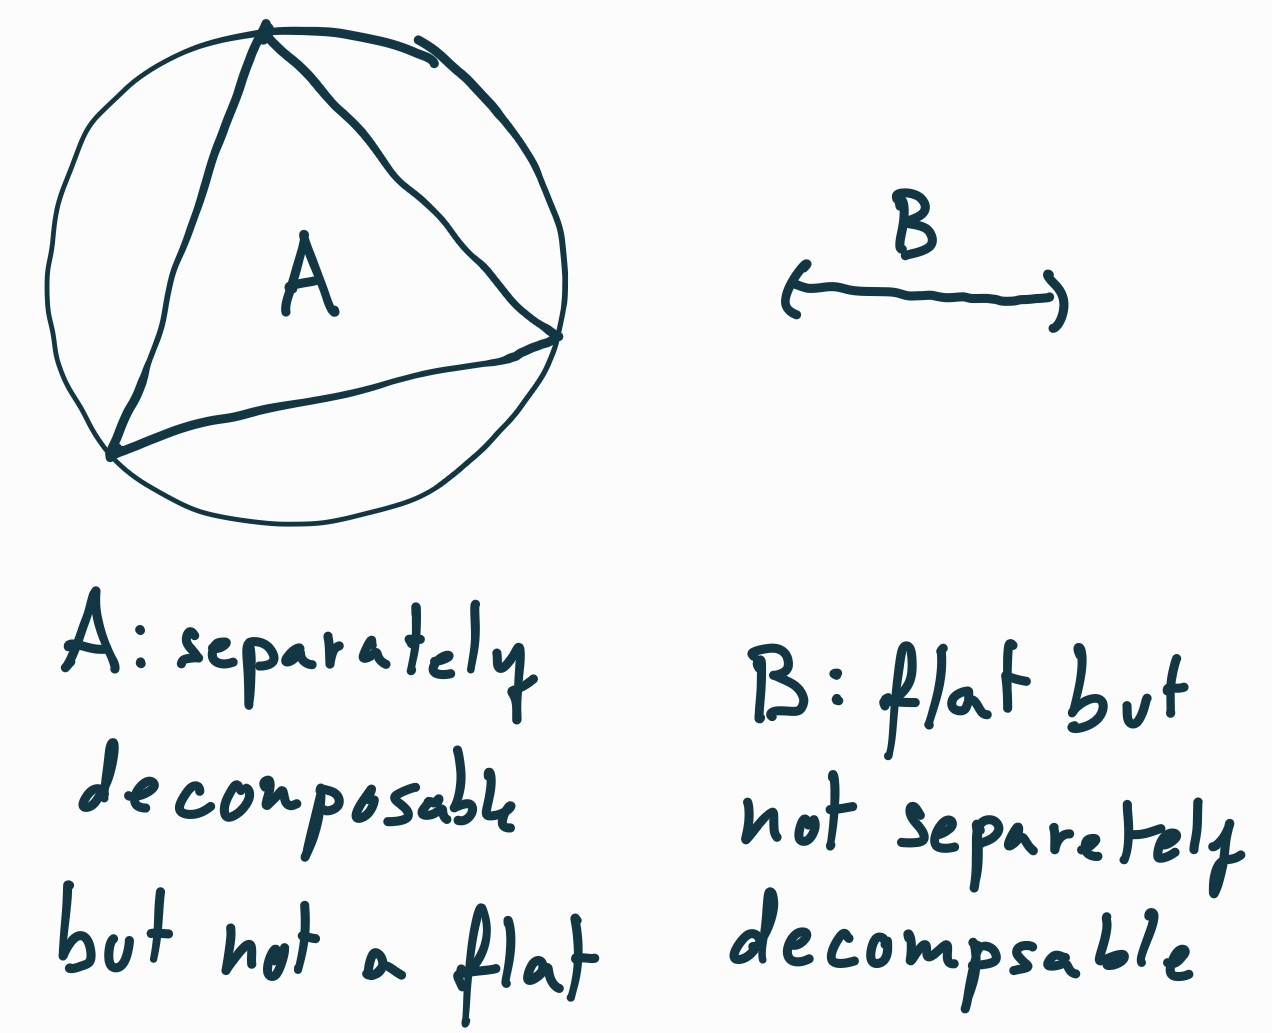
\includegraphics[width=0.4\textwidth]{tempimages/SeparableButNotFlat.jpg}
\end{figure}

\begin{remark}
	A convex set that is separately decomposable is not necessarily a flat (i.e. triangle within a sphere). A flat is not necessarily separately decomposable (i.e. open segment as a whole is a flat, but is not separately decomposable).
\end{remark}

\begin{defn}
	Let $\Ens$ be an ensemble space. A \textbf{classical probability context} is a flat $C \subseteq \Ens$ where each decomposable element in $C$ is separately decomposable in $C$ but not separately multidecomposable in $C$.
\end{defn}

\begin{prop}
	Let $C \subseteq \Ens$ be a classical probability context. Let $U \subseteq C$ be a set of ensembles. Then $A=U^\separate=\{ \ens[a] \in C \, | \, \forall \ens \in U, \ens[a] \separate \ens \}$ and $B=(U^\separate)^\separate=\{ \ens[b] \in C \, | \, \forall \ens[a] \in A, \ens[b] \separate \ens[a] \}$ are two probability contexts whose closed convex closure is $C$.
\end{prop}

\begin{proof}
	First we show that $C$ contains only three types of ensembles: those that are limits of convex mixtures of $A$, those that are limits of convex mixtures of $B$ and those that are limits of convex mixtures of both $A$ and $B$. Any ensemble in $C$ is one of these three types. For $\ens[c] \in C$ to not be a mixture of $A$ or $B$, then $\ens[c]$ cannot be in either $A$ or $B$. This means that it must be separate from both $A$ and $B$. But $B$ contains all the elements that are separate from $A$, which is a contradiction. Since separate multidecomposition is forbidden, an ensemble $\ens$ cannot be written both as a convex combination of $A$ and as a convex combination with an element of $B$. This would yield two decompositions in which one component, the one chosen from $B$, is separate from the all the components of the other. This means that an element of $C$ is either a mixture of $A$, a mixture of $B$ or a mixture of both $A$ and $B$.
	
	Now we show that both $A$ and $B$ are convex sets. Since a mixture of $A$ can only be expressed as a mixture of components of $A$, it is separate from all elements of $B$. Therefore $A$ contains all its mixtures. With the same logic, $B$ will contain all its mixtures. The argument works for infinite convex combinations as well. If $\ens = \sum_{i=1}^{\infty} p_i \ens[a]_i$, it can be understood as the limit of the series $\frac{p_1}{P_n} \ens[a]_1 + \frac{\bar{p}_1}{P_n} \sum_{i=2}^{n} p_i \ens[a]_i$ where $P_n = \sum_{i=1}^{n} p_i$. Therefore
	\begin{equation}
		\begin{aligned}
			\ens &= \sum_{i=1}^{\infty} p_i \ens[a]_i = \lim\limits_{n \to \infty}  \sum_{i=1}^{n} \frac{p_i}{P_n} \ens[a]_i = \lim\limits_{n \to \infty} \frac{p_1}{P_n} \ens[a]_1 + \lim\limits_{n \to \infty}\frac{\bar{p}_1}{P_n} \sum_{i=2}^{n} \frac{p_i}{\bar{p}_1} \ens[a]_i = p_1 \ens[a]_1 + \bar{p}_1 \sum_{i=2}^{\infty} \frac{p_i}{\bar{p}_1} \ens[a]_i \\
			&= p_1 \ens[a]_1 + \bar{p}_1 \hat{\ens[a]}_1
		\end{aligned}
	\end{equation}
	where $\hat{\ens[a]}_1 = \sum_{i=2}^{\infty} \frac{p_i}{\bar{p}_1} \ens[a]_i$. Since $\ens$ and $\ens[a]_1$ are elements of the ensemble space, the series converges to $\hat{\ens[a]}_1$, which is in the closed convex closure of $A$. It will also be an element of $A$ because multidecompositions are forbidden.
	
	To see that $C$ is the closed convex closure of $A$ and $B$, note that all the elements in $C$ that are not already in $A$ or $B$ are the mixtures of $A$ and $B$. These are exactly added when performing the closure.
	
	Now we show that $A$ and $B$ are classical probability contexts. First we have to show that they are flats. Let $L$ be the line that connects two elements $\ens[a]_1, \ens[a]_2 \in A$. Take $\ens[a]_3 \in L$. If it is a mixture of $\ens[a]_1$ and $\ens[a]_2$ then it is an element of $A$. If $\ens[a]_1$ is a mixture of $\ens[a]_2$ and $\ens[a]_3$, since $\ens[a]_1$ cannot have a common component with $B$, and $\ens[a]_3$ is a component of $\ens[a]_1$, $\ens[a]_3$ cannot have components in $B$ as well. Therefore $\ens[a]_3$ must be a mixture of elements of $A$. Similarly if $\ens[a]_2$ is a mixture of $\ens[a]_1$ and $\ens[a]_3$. Therefore $A$ is a flat. Similarly, $B$ is a flat.
	
	Now we show that $A$, and by symmetry $B$, is a classical probability context. We have seen that $A$ is a flat. If an element of $A$ is decomposable in $A$, it is also separately decomposable in $A$. In fact, if an element of $A$ is decomposable in $A$ it is also decomposable in $C$ and is therefore separately decomposable in $C$. Because multidecomposability in $C$ is not allowed, it must be separately decomposable in elements of $A$. Lastly, if multidecomposability were allowed in $A$, it would also be allowed in $C$. Therefore it is not allowed in $A$. This means that $A$ is a classical probability context.
\end{proof}

\begin{figure}[h]
	\centering
	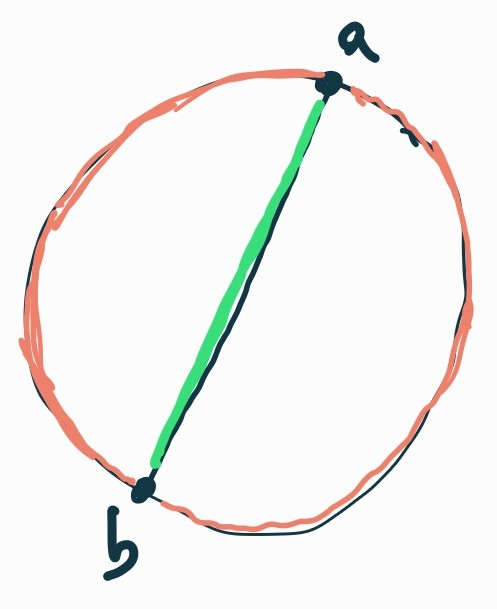
\includegraphics[width=0.25\textwidth]{tempimages/CounterexampleProbabilityContexts.jpg}
	\caption{TODO: make the final picture not go through the center}
\end{figure}

\begin{remark}
	Note that if multiple separate decompositions are not ruled out, the sub-contexts will not include all convex combinations. Take a disk as a convex space. Suppose $U$ is made of two points $a$ and $b$. All other points on the surface are separate from both and therefore belong to $A$. Now consider the convex combinations of $a$ and $b$. These are not separate from $U$ but they are also not separate from all the other elements on the surface. Therefore they are neither in $A$ nor $B$. Moreover, any other point in the interior can be seen as a convex combination of $a$ and another element of the surface that is not $b$. Therefore no point in the interior is in either $A$ or $B$. Thus $A$ and $B$ are not necessarily convex sets if $C$ is not a classical probability context.
\end{remark}

\begin{figure}[h]
	\centering
	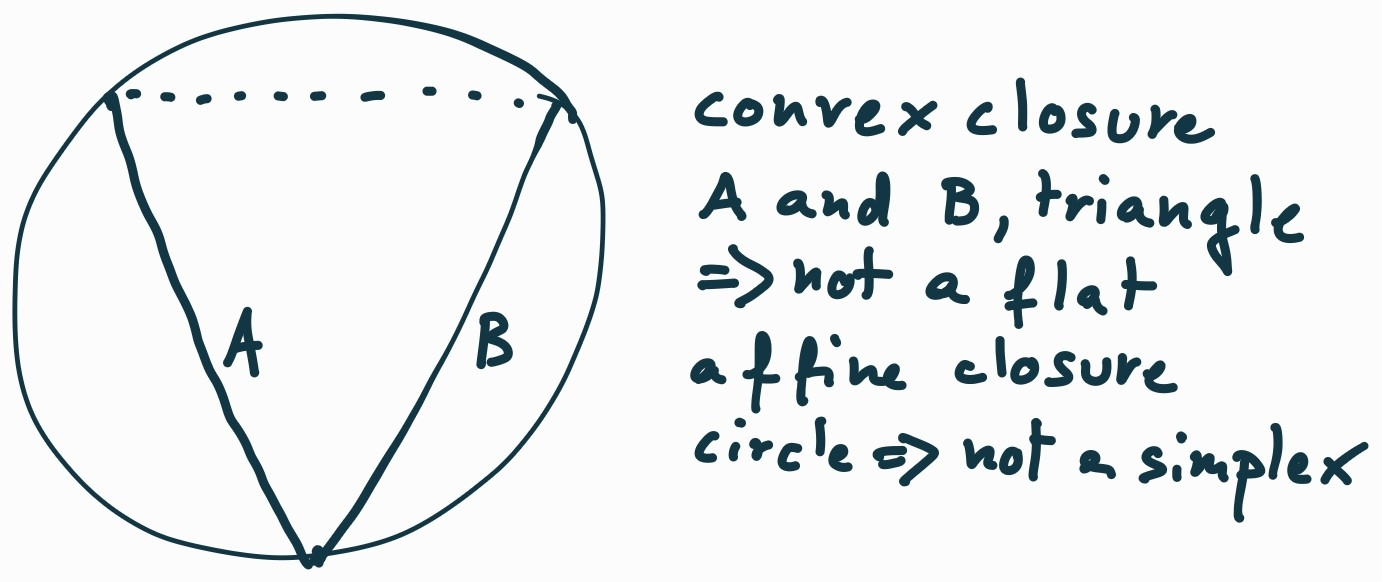
\includegraphics[width=0.75\textwidth]{tempimages/ContextClosureNotContext.jpg}
\end{figure}

\begin{remark}
	While a classical probability context can be decomposed into classical probability contexts whose closure is the original context, the converse is not true. That is, given two classical probability contexts, their convex or flat closure is not in general a classical probability context. Take a disk (the ensemble space) and two lines connecting three points (the two probability contexts). The convex closure is the triangle, which is not a flat as it misses some affine combinations. The flat closure is the disk, which is not a probability context.
\end{remark}

\begin{conj}
	Let $A, B \subseteq \Ens$ be two classical probability contexts. Then their flat closure and convex closure coincide if and only if they are a classical probability context.
\end{conj}

\begin{conj}
	The defining property of a classical probability context is exactly that property that allows $A$ and $B$ so constructed to be convex sets whose closure is $C$.
\end{conj}

\begin{prop}
	Let $C \subseteq \Ens$ be a classical probability context. Let $\mathfrak{L}$ be the lattice of $\separate$-subspaces. Then the fraction capacity is an additive set function on the lattice. That is, for all $\ens \in C$ and $A, B \in \mathfrak{L}$ such that $A \cap B = \emptyset$,  $\fcap_{\ens}(A \vee B) = \fcap_{\ens}(A) + \fcap_{\ens}(B)$.
\end{prop}

\begin{proof}
	Let $A, B\in \mathfrak{L}$ such that $A \cap B = \emptyset$. Then $A$ is separate from $B$. Therefore $A \vee B$ is a classical probability context that is the convex closure of two separate probability contexts. Therefore, as we saw in a previous proof, $A \vee B$ consists of convex combinations of $A$, which are all in $A$, of convex combinations of $B$, which are all in $B$, and of convex combinations of both, which are in neither $A$ nor $B$.
	
	We want to show that $\fcap_{\ens}(A \vee B) = \fcap_{\ens}(A) + \fcap_{\ens}(B)$ if $\ens \in A \vee B$. Let $\ens \in A \vee B$ be an ensemble that is the mixture of elements of $A$. Then $\ens \in A$ and it has no components in $B$. Therefore $\fcap_{\ens}(A \vee B) = 1$ and $\fcap_{\ens}(A) = 1$ while $\fcap_{\ens}(B) = 0$. Which means $\fcap_{\ens}(A \vee B) = 1 = 1 + 0 = \fcap_{\ens}(A) + \fcap_{\ens}(B)$. If $\ens$ is a mixture of elements of $B$, we get the same conclusion. The last case is when $\ens$ is a mixture of elements of $A$ and $B$. That is, $\ens = \sum_i p_i \ens[a]_i + \sum_j \lambda_j \ens[b]_j$ with $\ens[a]_i \in A$, $\ens[b]_j \in B$, $p_i, \lambda_j \in [0,1]$ and $\sum_i p_i + \sum_j \lambda_j = 1$. By definition of fraction capacity, $\sum_i p_i \leq \fcap_{\ens}(A)$. Suppose $\sum_i p_i < \fcap_{\ens}(A)$. Then there is $\hat{\ens[a]} \in A$ such that $\ens = \sum_i p_i \ens[a]_i + p \hat{\ens[a]} + \lambda \ens[c]$ for some $p,\lambda \in [0,1]$ and $\ens[c] \in A \vee B$. But then $\ens$ would be separately multidecomposable, which is a contradiction since it is an element of a classical probability context. Therefore $\sum_i p_i = \fcap_{\ens}(A)$. Similarly, we find that $\sum_j \lambda_j = \fcap_{\ens}(B)$. Since $\sum_i p_i + \sum_j \lambda_j = 1$, $\fcap_{\ens}(A) + \fcap_{\ens}(B) = 1 = \fcap_{\ens}(A \vee B)$ for all $\ens \in A \vee B$.
	
	Now let $\ens \in C$. We have $(A \vee B)^\separate \in \mathfrak{L}$ and $(A \vee B) \cap (A \vee B)^\separate = \emptyset$. Therefore $\fcap_{\ens}(C) = \fcap_{\ens}(A \vee B)+ \fcap_{\ens}((A \vee B)^\separate)$. Note that $\ens$, in general, is a convex combination of elements of $A\vee B$ and $(A \vee B)^\separate$. Components in $A \vee B$ are convex combinations of elements of $A$ and $B$, which also disjoint. Therefore $\ens$ is a convex combination of elements of $A$, $B$ and $(A \vee B)^\separate$, which are pairwise disjoint. As before, since multidecomposability is forbidden in a classical probability context, the sum of the coefficients for each part will have to match the fraction capacity of its subcontext. Therefore $\fcap_{\ens}(A) +  \fcap_{\ens}(B) + \fcap_{\ens}((A \vee B)^\separate) = \fcap_{\ens}(C) = \fcap_{\ens}(A \vee B) + \fcap_{\ens}((A \vee B)^\separate)$. Thus $\fcap_{\ens}(A \vee B) = \fcap_{\ens}(A) +  \fcap_{\ens}(B)$ for all $\ens \in C$.
\end{proof}

% Reviewed with Christine end

We now want to define a notion of spectra for a classical probability context. These will constitute the sample space over the measures are defined. We will use the notion of subspaces defined in \ref{pm_es_subspaceSection} and applied to separateness.

\begin{defn}
	Given a classical probability context $C \subseteq \Ens$, the \textbf{spectra} $\sigma(C)$ is the set of equivalence classes of ensemble sequences that are eventually separate from each other. More rigorously, given a probability context, the spectra is the collection of the ultrafilters of the lattice of $\separate$-subspaces $\mathfrak{L}^\separate(C)$. The standard topology of the spectra is the one generated by the complements of the elements of the lattice seen as a set (i.e. for each $A \in \mathfrak{L}^\separate(C)$, $A \mapsto \{ x \in \Sigma(C) \, | \, A \in x \}$).
\end{defn}

\begin{prop}
	Let $\Ens$ be a discrete classical ensemble space. Then $\Ens$ is a probability context, the spectra is the sample space and its topology is the discrete topology.
\end{prop}

\begin{proof}
	Let $\Ens$ be a discrete classical ensemble space. The whole space is a flat as it contains all its affine combinations. Note that two ensembles are separate if and only if they have disjoint support. Suppose $\ens = p \ens[a]_1 + \bar{p} \ens[a]_2 = \lambda \ens[b]_1 + \bar{\lambda} \ens[b]_2$. Then the union of the support of each pair must be the same. Therefore the support at least one element of each pair must overlap with the support of another element of another pair. This means that separate multidecomposability is not allowed. Therefore $\Ens$ is a classical probability context.
	
	Since ensembles are separate if and only if they have disjoint support, the $\separate$-closure of a subset $A \subseteq \Ens$ of ensembles corresponds to all ensembles whose support is a subset of the union of the supports of the elements of $A$. Each $\separate$-subspace, then, is associated to one unique subset $U \subseteq \Omega$ of the sample space. Given that for any subset $U$ we can find a measure whose support is $U$, every subset corresponds a unique $\separate$-subspace. If the support of a measure is a subset of $U$, it will also be a subset of any other set $V \supseteq U$. Therefore the ordering of the lattice of $\separate$-subspaces is the same as inclusion on the lattice of supports. The two lattices are isomorphic.
	
	Since the singletons are elements of the lattice, all ultrafilters are principal, meaning that they are all of the form $X(x) = \{A \in \mathfrak{L}^\separate(C) \, | \, \{x\} \in A\}$ where $x \in \Omega$ is an element of the sample space. Therefore the sample space and the spectra coincide. Each singleton is a closed set, since it is an element of the lattice. The complement of each singleton is also an element of the lattice, therefore each singleton is also an open set. The topology is therefore the discrete topology.	
\end{proof}

\begin{remark}
	Note that the union of two open sets of $\sigma(C)$ is not the same as the join in the lattice of $\separate$-subspaces.
\end{remark}

\begin{remark}
	TODO: organize. There are different types of limits. One limit of convex combinations. Physically, these are mixtures over infinitely many elements. Limit of ensemble sequences. Physically, these are sequences of ensembles, taken one after the other, for example in temporal succession. Limits of ensembles taken from $\separate$-subspaces strictly included into each other. This is the limit of ensemble that are finer and finer.
\end{remark}

\begin{defn}
	Let $X$ be a topological space. We say a measure $\mu : \Sigma_X \to \mathbb{R}$ is continuous with respect to the topology if $\mu(A) = \mu(\bar{A})$. Equivalently, all boundaries are measure zero.
\end{defn}

\begin{prop}
	A classical probability context can be represented by a set of measures over its spectra that are continuous with respect to its topology.
\end{prop}

\begin{proof}
	Let $C \subseteq \Ens$ be a classical probability context, $\sigma(C)$ its spectra and $\textsf{T}$ its topology. Recall that the topology is generated by sets corresponding to the lattice $\mathfrak{L}^\separate(C)$. By the Carathéodory extension theorem, there is a unique way to extend a pre-measure on that lattice to the whole Borel algebra. For each element $\ens \in C$, then, we can find a unique measure on the Borel algebra of $\sigma(C)$ that coincides with the fraction capacity on a basis of the topology.
	
	Let $A \in \mathfrak{L}^\separate(C)$ correspond to an element of the lattice. Then $A^\separate$ is the largest $\separate$-subsapce that is disjoint from $A$. Since $A$ corresponds to an open set, $A^\separate$ corresponds to its exterior. Since $\fcap_{\ens}(A) + \fcap_{\ens}(A^\separate) = 1$, the measure over the boundary of $A$ is zero. Since this is valid for any element of the basis, it will be valid for any open set and consequently for any Borel set. Therefore each element $\ens$ corresponds to a measure where all boundaries are of measure zero.
\end{proof}

\begin{prop}
	A convex subset $U \subset \Ens$ is a classical probability context if and only if it is the subset of probability measures of a vector space of measures over a sample space $\Omega$.
\end{prop}

\begin{prop}
	A convex subset $U \subset \Ens$ is a classical probability context if and only all finite flats a simplexes.
\end{prop}

\begin{proof}
	Let $\ens = p \ens[a] + \bar{p} \ens[b] = \lambda \ens[c] +\bar{\lambda} \ens[d]$
\end{proof}

\begin{coro}
	Classical discrete and classical continuous ensemble spaces are classical probability spaces.
\end{coro}

\begin{proof}
	For a classical discrete ensembleBoth spaces are defined as the convex spaces of probability measures.
\end{proof}

\begin{prop}[Separatedness extends on all mixtures]\label{pm_es_separateExtendsMixtures}
	Let $\ens,\ens_1,\ens_2 \in \Ens$. If $\ens$ has no common component with a mixture of $\ens_1$ and $\ens_2$ then it has no common component with any mixture of $\ens_1$ and $\ens_2$ and with either $\ens_1$ and $\ens_2$. That is, if $\ens \separate p \ens_1 + \bar{p} \ens_2$ for some $p \in (0, 1)$ then $\ens \separate p \ens_1 + \bar{p} \ens_2$ for all $p \in [0, 1]$.
\end{prop}

\begin{figure}[h]
	\centering
	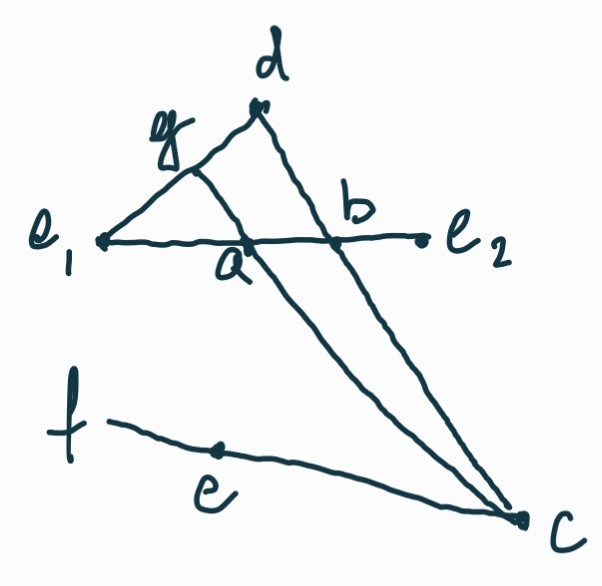
\includegraphics[width=0.3\textwidth]{tempimages/DistinctAndMixture.jpg}
\end{figure}

\begin{proof}
	Let $\ens \separate \ens[a] = p \ens_1 + \bar{p} \ens_2$ for some $p \in (0, 1)$. Let $\ens[b] = \alpha \ens_1 + \bar{\alpha} \ens_2$ with $0 \leq \alpha < p$. We can do so without loss of generality since switching $\ens_1$ with $\ens_2$ would lead to the case where $1 \geq \alpha > p$. Suppose $\ens[b]$ is not separate from $\ens$. Then we can find $\ens[c] \in \Ens$ such that $\ens[b] = \beta \ens[c] + \bar{\beta} \ens[d]$ and $\ens = \gamma \ens[c] + \bar{\gamma} \ens[f]$ for some $\ens[d], \ens[f] \in \Ens$ and $\beta, \gamma \in (0, 1)$.
	
	Setting $\epsilon = \frac{p - \alpha}{\bar{\alpha}}$ and $\lambda = \bar{\epsilon} \beta$ we have:
	\begin{align*}
		\ens[a] &= p \ens_1 + \bar{p} \ens_2 = \left(p - \frac{\bar{p}}{\bar{\alpha}} \alpha \right) \ens_1 + \frac{\bar{p}}{\bar{\alpha}} \alpha \ens_1 + \frac{\bar{p}}{\bar{\alpha}} \bar{\alpha}\ens_2 \\
		&= \left(\frac{p\bar{\alpha} - \bar{p}\alpha}{\bar{\alpha}} \right) \ens_1 + \frac{\bar{p}}{\bar{\alpha}} (\alpha \ens_1 + \bar{\alpha} \ens_2) = \left(\frac{p - p\alpha - \alpha + p \alpha}{\bar{\alpha}} \right) \ens_1 + \frac{1 - p + \alpha - \alpha}{\bar{\alpha}} (\alpha \ens_1 + \bar{\alpha} \ens_2) \\
		&= \frac{p - \alpha}{\bar{\alpha}}  \ens_1 + \left( 1 - \frac{p - \alpha}{\bar{\alpha}}\right) (\alpha \ens_1 + \bar{\alpha} \ens_2) = \epsilon \ens_1 + \bar{\epsilon} (\alpha \ens_1 + \bar{\alpha} \ens_2) = \epsilon \ens_1 + \bar{\epsilon} \ens[b] \\
		&= \epsilon \ens_1 + \bar{\epsilon} ( \beta \ens[c] + \bar{\beta} \ens[d] ) = \bar{\epsilon} \beta \ens[c] + \epsilon \ens_1 + \bar{\epsilon} \bar{\beta} \ens[d] = \lambda \ens[c] + \bar{\lambda} \ens[g]
	\end{align*}
	where $\ens[g] = \frac{1}{\bar{\lambda}}\left( \epsilon \ens_1 + \bar{\epsilon} \bar{\beta} \ens[d] \right)$. This means $\ens[a]$ and $\ens$ have a common component, which is a contradiction. Therefore $\ens[b] \separate \ens$ and $\ens \separate p \ens_1 + \bar{p} \ens_2$ for all $p \in [0, 1]$.
\end{proof}

\begin{defn}
	We say that in an ensemble space $\Ens$ \textbf{mixtures preserve separatedness} if whenever an ensemble is separate from two other ensembles, than it is also separate from all their mixtures. That is, $\ens \separate \ens[a]$ and $\ens \separate \ens[b]$ implies $\ens \separate p \ens[a] + \bar{p} \ens[b]$ for all $p \in [0,1]$.
\end{defn}

\begin{conj}
	In a classical probability space mixtures preserve separatedness. In a quantum ensemble space mixtures do not preserve separatedness.
\end{conj}

\begin{proof}
	Let $\Ens$ be a classical probability space and let $\mu, \nu \in \Ens$ be probability measures on some space $\Omega$. The space of probability measures is a subset of the space of signed measures. This space can be equipped with an inner product. The space of signed measures with support $U \subseteq \Omega$ forms a subspace. This means that, if we can find a $U \subseteq \Omega$ such that both $\mu(U) \neq 0$ and $\nu(U) \neq 0$, we can find a probability measure that is a component of both. That is, two probability measures that have overlapping support have a common component. Conversely, given that convex combination can only expand the support of measures, two probability measures that have no overlapping support have no common components. (TODO: if all measure are allowed, we may get also measures we do not want - Dirac measures, measures that have no continuous derivative. If not all measures are allowed, we have no existence of a measure that can be a component, and therefore there may be overlapping measures that have no common components.)
	
	Now, suppose $\ens \separate \ens[a]$ and $\ens \separate \ens[b]$. This means that the support of $\ens$ is disjoint from the support of both $\ens[a]$ and $\ens[b]$, which will also be disjoint from the support of any mixture of $\ens[a]$ and $\ens[b]$ since the support of the mixture will be the union of the individual supports. This means that $\ens$ will be separate from all mixtures of $\ens[a]$ and $\ens[b]$. The property holds, then, in any classical ensemble space.
	
	On the other hand, suppose that $\Ens$ is a quantum ensemble space. Without loss of generality, suppose $\Ens$ is the Bloch sphere and consider the states $x^+$, $x^-$, $z^+$, and $z^-$, which are points on the surface that form a square. These are all separate ensembles. We have $\frac{1}{2} x^+ + \frac{1}{2} x^- = \frac{1}{2} z^+ + \frac{1}{2} z^-$. Therefore a mixture of $x^+$ and $x^-$ has a common component with $z^+$. That is, $z^+ \separate x^+$ and $z^+ \separate x^-$ but $z^+ \nseparate \frac{1}{2} x^+ + \frac{1}{2} x^-$.
\end{proof}

\begin{prop}
	Let $\Ens$ be an ensemble space where mixtures preserve separatedness. Then for every $\ens \in \Ens$ and any Borel set $A \subseteq \Ens$ we can find a sequence $\{a_i\} \subset \hull(A) $
\end{prop}

\begin{conj}
	Let $\Ens$ be an ensemble space where mixtures preserve separatedness. Then it is a classical probability space.
\end{conj}




\section{Statistical properties and quantities}

In the same way that we define ensembles first, we define quantities through their expectation over ensembles. The possible value for pure states will need to be recovered with constructions that are connected to spectral theory.

\begin{defn}
	A \textbf{statistical property}, or simply property, is an attribute that allows statistical handling. Formally, it is a continuous map $F : \Ens \to \mathcal{Q}$ where $\mathcal{Q}$ is a convex topological space such that $F(p \ens_1 + \bar{p} \ens_2) = p F(\ens_1) + \bar{p} F(\ens_2)$.
	
	A \textbf{statistical quantity}, or statistical variable, or simply variable, is a numerical statistical property. That is, it is a continuous linear real valued operator $F : \Ens \to \mathbb{R}$.
\end{defn}

\begin{justification}
	This definition extends the general definition of properties and quantities we already gave to the statistical case. As before, continuity is required since verifying the value of the quantity corresponds to verifying that we are dealing with a specific subset of ensembles.
	
	The ability to create convex combinations corresponds to the ability to create statistical averages. Therefore $\mathcal{Q}$ must be a convex set. Given that preparations are assumed to be independent, the a mixture of the preparation will produce a mixture of the properties according to the same fractions. 
	
	Quantities are simply properties that are linearly ordered. The ability to create convex combinations becomes the ability to take weighted averages of the quantities. Regardless of whether one starts from integers, rationals or real valued quantities, the statistical averages will, in general, be a real number.
	
	Note that the numerical value cannot be infinite. The only way to measure infinity is if the measured average keeps increasing in time. This would be a contradiction on the assumption that the ensemble is reproducible.
\end{justification}

\begin{remark}
	Note that variables will have a contiguous range on the ensembles because, given two ensembles with different values, we can mix them to obtain any intermediate value. This does not mean that the variable can take all possible values on pure states. For example, the number of particles in a pure state will necessarily be a non-negative integer, but we can mix those to create ensembles that have non-integer average number of particles.
\end{remark}

\begin{coro}
	A set of statistical quantities $\{F_i\}_{i \in I}$ can be collected into a single statistical property $F : \Ens \to \mathbb{R}^I$ where $F(\ens) = \{F_i(\ens)\}_{i \in I}$.
\end{coro}

\begin{prop}
	Let $\Ens$ be a classical probability space. Then each statistical quantity is the expectation of a random variable and vice-versa.
\end{prop}

\begin{proof}
	Let $\Ens$ be an ensemble space where each ensemble is a probability measure $\mu$ over some sample space $\Omega$. Let $f : \Omega \to \mathbb{R}$ be a random variable, then the expectation $F(\mu) = \int_{\Omega} f d\mu$ is a statistical quantity. Conversely, let $F : \Ens \to \mathbb{R}$ be a linear functional of the measures. Then, by (TODO: CHECK) Riesz representation theorem, we can write $F(\mu) = \int_{\Omega} f d\mu$ from some $f : \Omega \to \mathbb{R}$.
\end{proof}

\begin{conj}
	Let $\Ens$ be a quantum ensemble space. Then each statistical quantity is the expectation of an observable and vice-versa.
\end{conj}

\begin{proof}
	TODO: need to find a quantum correspondent of the Riesz representation theorem.
\end{proof}

\begin{conj}
	Let $e \in \Ens$ be an ensemble, $F : \Ens \to \mathbb{R}$ be a statistical variable and $A \subset \Ens$ be a set of ensemble. Let $\ens[a]_i$ and $\ens[b]_i$ be maximal $A$-component sequences of $\ens$. Then $\lim_{i \to \infty} F(\ens[a]_i) = \lim_{i \to \infty} F(\ens[b]_i)$.
\end{conj}

\begin{defn}
	Let $e \in \Ens$ be an ensemble, $F : \Ens \to \mathbb{R}$ be a statistical variable and $A \subset \Ens$ be a set of ensemble. Then the \textbf{contribution to $F$ over $A$ given $\ens$} is the limit of variable for a maximal $A$-component sequence of $\ens$. That is, $F_{\ens}(A) = \lim_{i \to \infty} F(\ens[a]_i)$ where $\ens[a]_i$ is a maximal $A$-component sequence of $\ens$.
\end{defn}

\begin{prop}
	The contribution to $F$ is a set function.
\end{prop}

\begin{proof}
	Since $F_{\ens}$ takes a set of an argument and returns a real value, is a set function.
\end{proof}

\begin{remark}
	Note that the contribution cannot be monotone in the same way that the expectation of a random variable to an event is not monotone. Not clear whether the additivity of the variable may tell us something about the additivity of the contribution.
\end{remark}

\begin{conj}
	We can define a ``derivative'' $f_{\ens}$ between $F_{\ens}$ and $\fcap_{\ens}$ such that $F_{\ens}(A) = \int_A f_{\ens} \, d \fcap_{\ens}$ where $\int$ is the ??? integral.
\end{conj}

\begin{remark}
	This may still not be the correct formulation of the problem. Note that $A$ is a set of ensembles. In the classical case it would correspond to a set of probability measures, not a subset of the sample space (i.e. an event). However, in the discrete case and in the quantum case, $A$ can also be restricted to a set of pure state (i.e. extreme points), which would correspond to a subset of the sample space. It may be worth at least understanding that case.
\end{remark}

\subsection{Quantifiable spaces and locally convex vector spaces}

\begin{prop}
	Let $\Ens$ be a complemented ensemble space. Then a statistical variable $F$ induces a semi-norm on the vector space that embeds $\Ens$.
\end{prop}

\begin{proof}
	Let $F$ be a variable on $\Ens$ and let $V$ be the vector space that embeds $\Ens$. Extend $F$ on $V$ such that $F(a\ens) = |a| F(\ens)$. Then, according to the definition given after 1.1 in \url{https://personal.math.ubc.ca/~cass/research/pdf/TVS.pdf} $F$ is a semi-norm.
\end{proof}

\begin{defn}
	A \textbf{quantifiable} ensemble space is an ensemble space where each ensemble can be identified by a set of statistical variables. That is, there is family of statistical variables $F_i : \Ens \to \mathbb{R}$ such that, given $\ens_1, \ens_2 \in \Ens$, $F_i(\ens_1) = F_i(\ens_2)$ for all $i$ if and only if $\ens_1 = \ens_2$. Moreover, the topology is generated by those variables.
\end{defn}

\begin{prop}
	A quantifiable ensemble space is complemented and embeds into a Hausdorff locally convex topological vector space.
\end{prop}

\begin{proof}
	Let $\ens[a], \ens[b], \ens[c] \in \Ens$ be three ensembles such that $p \ens[a] + \bar{p} \ens[b] = p \ens[a] + \bar{p} \ens[c]$ for some $p \in (0,1)$. For any statistical variable $F : \Ens \to \mathbb{R}$ we have
	\begin{equation}
		\begin{aligned}
			F(p \ens[a] + \bar{p} \ens[b]) &= F(p \ens[a] + \bar{p} \ens[c]) = p F(\ens[a]) + \bar{p} F(\ens[b]) = p F(\ens[a]) + \bar{p} F(\ens[c])\\
			F(\ens[b]) &= F(\ens[c]) 
		\end{aligned}
	\end{equation}
	For a quantifiable ensemble space with statistical variables $F_i$, we have $F_i(\ens[b]) = F_i(\ens[c])$, which means $\ens[b] = \ens[c]$. Since $\ens[a]$, $\ens[b]$, $\ens[c]$ and $p$ where arbitrary, the space is complemented.
	
	The ensemble is complemented, therefore it is embedded into a vector space. The topology of the ensemble space is generated by the statistical variables, which induce semi-norms on the vector space. This means that the topology of the vector space is generated by a countable set of semi-norms, and is therefore a locally convex topological vector space. See Prop 2.2 in \url{https://personal.math.ubc.ca/~cass/research/pdf/TVS.pdf}.
	
	The statistical variables fully identify each ensemble, which means that, if two elements are different, one semi-norm will give a non-zero value for the distance function associated with it. This means that the topology is Hausdorff. See Prop 2.6 in \url{https://personal.math.ubc.ca/~cass/research/pdf/TVS.pdf}.
\end{proof}

\begin{coro}
	A quantifiable ensemble spaces is fully determined by countably many statistical variables.
\end{coro}

\begin{proof}
	The topology of an ensemble space is second countable. A Hausdorff second countable locally convex topological vector space can always be generated by countably many semi-norms.
\end{proof}

\begin{remark}
	Note that we are missing completeness in terms of the semi-norms to obtain a Fr\'echet space. It is not clear whether this is required since, for example, $L^1(\mathbb{R}^{2n}) \cap C(\mathbb{R}^{2n})$ is not Fr\'echet.
\end{remark}

\begin{conj}
	Discrete/continuous classical ensemble spaces and quantum ensemble spaces are quantifiable.
\end{conj}

\begin{proof}
	For discrete classical spaces, the expectation of the indicator of each extreme point defines a countable set of quantities that fully identifies the distribution.
	
	For continuous classical spaces, $L^1(\mathbb{R}^{2n}) \cap C(\mathbb{R}^{2n})$ is a Hausdorff locally convex topological spaces.
	
	TODO Quantum (note that we are looking at the space of density operators with finite expectation value for position and momentum).
\end{proof}

\begin{conj}
	If all ensembles can be connected by linear transformations parameterized by real quantities, then the ensemble is quantifiable.
\end{conj}

\begin{remark}
	Note clear whether this is true. The idea is that the time interval can be used to define variables. A more sophisticated conjecture may look at the space of generators of Lie groups. This would link the topology of time to the topology of the ensemble space. If the topology of time is not that of the real numbers, then, the ensemble space must change significantly.
\end{remark}

% TODO: for later
%\begin{conj}
%	Let $\ens \in \Ens$ and $A \subset \Ens$. Let $\{\ens[a]_i\}$ and $\{\ens[b]_i\}$ be two maximal increasing $A$-component sequence. Then $\lim\limits_{i \to \infty} F(\ens[a]_i) = \lim\limits_{i \to \infty} F(\ens[a]_i)$ for any quantities $F$.
%\end{conj}

\begin{proof}
	Check that the all maximal sequences give the same value.
\end{proof}

\subsection{Macrostates and thermodynamics}

TODO: This should be moved after the definition of entropy.

In this section we try to recover some elements of thermodynamics on the generalized ensemble space. We want to recover Gibbs' thermodynamics, which means an equation of state in terms of extensive quantities. Instead of extensive quantities, we are going to use statistical quantities. Note that the idea that all extensive quantities are statistical (i.e. the average during mixing) seems to work. The energy and the number or particles average during mixture. The idea that volume averages during mixture can be understood as the system oscillating between the different volumes defined by the components. It also seems that intensive quantities do not average during mixing. Temperature, for example, is only defined on equilibria (i.e. of Boltzmann distributions) and the mixture of two equilibria at different temperature is not an equilibrium. Still, we would need a general proof, which would require the notion of product spaces (i.e. intensitive/extensive quantities represent system/subsystem relationship).

\begin{defn}
	Let $\Ens$ be an ensemble space. Let $F : \Ens \to \mathcal{Q}$ be a statistical property. The \textbf{coarse graining} of $\Ens$ over $F$ is the set $\mathcal{M} \subseteq \Ens$ represented by the ensemble that maximize the entropy for each fixed value of the property. That is, there exists a map $\psi : \mathcal{Q} \to \mathcal{M}$ such that $F(\psi(x)) = x$ and $S(\psi(x)) \geq \ens$ for all $\ens \in \Ens$ such that $F(\ens) = x$. The \textbf{equation of state} is the map $S(x) \mapsto S(\psi(x))$ that returns the entropy given the value of the statistical property.
\end{defn}

\begin{conj}
	Let $F : \Ens \to \mathbb{R}^n$ be a vector of statistical quantities. Then the corresponding coarse graining of $\mathcal{M}$ is a manifold. The equation of state $S : \mathbb{R}^n \to \mathbb{R}$ returns the entropy as a function of the statistical values.
\end{conj}

\begin{remark}
	We need to prove that $\mathcal{M}$ inherits the topology from $\Ens$. Are we be able to recover the topological isolation of phase transitions? The quantities will typically be energy plus other extensive quantities (i.e. volume, number of particles, ...).
\end{remark}

\begin{prop}
	The equation of state is strictly concave. That is, $S(\lambda x + \bar{\lambda} y) \geq \lambda S(x) + \bar{\lambda} S(y)$ and the equality holds if and only if $x=y$.
\end{prop}

\begin{proof}
	Let $x, y \in \mathcal{Q}$ be two possible values for the statistical property, and let $\lambda x + \bar{\lambda} y$ be a convex combination. We have $F(\psi(\lambda x + \bar{\lambda} y)) = \lambda x + \bar{\lambda} y = F(\lambda \psi(x) + \bar{\lambda} \psi(y))$. That is, $\psi(\lambda x + \bar{\lambda} y)$ and $\lambda \psi(x) + \bar{\lambda} \psi(y)$ are two ensembles that share the same value for the statistical property. By definition, the entropy of the first cannot be lower than the entropy of the second. We have
	\begin{equation}
		\begin{aligned}
			S(\lambda x + \bar{\lambda} y) &= S(\psi(\lambda x + \bar{\lambda} y)) \\
			&\geq S(\lambda \psi(x) + \bar{\lambda} \psi(y)) \\
			&\geq \lambda S(\psi(x)) + \bar{\lambda} S(\psi(y)) \\
			&= \lambda S(x) + \bar{\lambda} S(y),
		\end{aligned}
	\end{equation}
	which shows that the equation of state is concave.
	
	Now suppose that $x=y$. Then on one side $S(\lambda x + \bar{\lambda} y) = S(x)$ and on the other side $\lambda S(x) + \bar{\lambda} S(y) = S(x)$. $S(\lambda x + \bar{\lambda} y) = \lambda S(x) + \bar{\lambda} S(y)$. Conversely, suppose that $x\neq y$. Then $\psi(x) \neq \psi(y)$. By the strict concavity of the entropy, we have
	\begin{equation}
		\begin{aligned}
			S(\lambda x + \bar{\lambda} y) &= S(\psi(\lambda x + \bar{\lambda} y)) \\
			&\geq S(\lambda \psi(x) + \bar{\lambda} \psi(y)) \\
			&> \lambda S(\psi(x)) + \bar{\lambda} S(\psi(y)) \\
			&= \lambda S(x) + \bar{\lambda} S(y),
		\end{aligned}
	\end{equation}
	which shows that the equation of state is strictly concave.
\end{proof}

\begin{remark}
	In the case of thermodynamics, where the statistical property is a vector of statistical values, the equation of state will be concave in all arguments and in all combination of arguments.
\end{remark}


\subsection{Spectra of a quantity}

This is an attempt to define spectra purely on the topology and the convex structure, without reference to entropy and therefore inner product structure. It is unclear whether this is possible. If it is not possible, this attempt is still useful to understand what are the required definitions.

\begin{defn}
	Let $\Ens$ be an ensemble space and let $F : \Ens \to \mathbb{R}$ be a statistical quantity. Let $U \subset \mathbb{R}$ an open set of possible values for the quantity. We define the set of \textbf{ensembles supported by $U$} as the convex set $A \subset \Ens$ such that for any component $\ens$ of any element $\ens[a] \in A$ $F(\ens) \in U$. That is, they are all the elements that can be mixed among each other and still have all components have an expectation that fall within $U$.
\end{defn}

\begin{remark}
	Note that even if we have $F(\ens) \in U$ for some $\ens$, we can still have that no ensemble is supported by $U$. Consider a simply two dimensional discrete classical space $p\ens[a] + \bar{p} \ens[b]$ with $F(\ens[a]) = 0$ and $F(\ens[b]) = 1$. Now consider $U = \left(\frac{1}{4}, \frac{3}{4} \right)$. Ensembles for which $F(\ens) \in U$ are necessarily mixtures of $\ens[a]$ and $\ens[b]$, and $F(\ens[a])\neq 0 \neq F(\ens[b])$. Therefore no ensemble is supported by $U$.
	
	On the other hand, even if we have ensembles for which the expectation for all the components falls in $U$, they may still not be supported by $U$. Consider a Bloch ball for a qubit and  $F : \Ens \to \mathbb{R}$ such that $F(|0\>\<0|) = 0$ and $F(|1\>\<1|) = 1$. We have $F(|+\>\<+|) = F(|-\>\<-|) = \frac{1}{2}$ and therefore any mixture of those states
\end{remark}

\begin{defn}
	Given a statistical quantity $F : \Ens \to \mathbb{R}$, its \textbf{spectrum} $\sigma(F) \subseteq \mathbb{R}$ is the set of values $f \in \mathbb{R}$, called \textbf{spectral elements}, such that the set of ensembles supported by an open set that contains $f$ is non-empty.
\end{defn}

\begin{prop}
	
\end{prop}

\begin{conj}
	We recover an equivalent notion of spectra for both classical and quantum mechanics.
\end{conj}

Note that, in principle, the definitions only use $\mathbb{R}$ as a topological space (that also has a convex structure). Maybe this can generalize in the case that quantities are not real numbers.

\section{Reducibility}

\subsection{Reducible ensemble spaces}

\begin{defn}
	An ensemble space $\Ens$ is \textbf{reducible} if separate ensembles are also orthogonal. That is, $\ens_1 \separate \ens_2$ implies $\ens_1 \ortho \ens_2$.
\end{defn}

\begin{justification}
	Given that $\ens_1 \ortho \ens_2$ implies $\ens_1 \separate \ens_2$, classical spaces add the opposite implication. Therefore they exclude the case where two ensembles are orthogonal but not separate. This case describes two ensembles that have elements in common, but there is no ensemble corresponding to those common elements. That is, we cannot refine the ensembles into three separate ones: one with only elements of the first, one with only elements of the second and one with elements of both. In other words, we cannot reduce the coarser description of the system into finer separate descriptions. In the excluded case, then, the coarser description is irreducible into finer ensembles. This justifies the definition.
	
	As we prove below, that case does not exist in classical mechanics, but exists in quantum mechanics. This justifies calling the property classical.
\end{justification}

\begin{prop}
	Continuous and discrete classical ensemble spaces are reducible.
\end{prop}

\begin{proof}
	In both cases, ensembles are probability measures: the first over the Borel algebra of a symplectic manifold; the second over the power set of countably many elements. In both cases, the upper bound of the entropy is maximized if and only if the probability measures being combined have disjoint support. This means that two ensembles are orthogonal if and only if the respective probability measures have disjoint support. Intuitively, two probability distributions can have a common sub-distribution if and only if they overlap. Therefore two ensembles representing probability measures with disjoint support are exactly ensembles that are separate. Therefore, in both cases, the ensemble space is reducible.
\end{proof}

\begin{conj}
	An ensembles space is reducible only if it is classical.
\end{conj}

\begin{remark}
	The reverse direction cannot, in general, work. Take the subspace of a finite classical discrete ensemble space such the maximum probability of any element is $k < 1$. This corresponds to a simplex of the same dimension, with the same center, but scaled in the interior. Given that it is a convex subset of an ensemble space, it will satisfy all the axioms, except it will contain no orthogonal ensembles. Yet, it contains separate ensembles, which cannot be orthogonal.
\end{remark}

\section{State capacity}

\begin{prop}[Exponential entropy subadditivity]\label{pm_es_exponentialEntropySubadditivity}
	Let $\ens_1, \ens_2 \in \Ens$. Let $S_1 = S(\ens_1)$ and $S_2 = S(\ens_2)$. Let $\ens = p \ens_1 + \bar{p} \ens_2$ for some $p \in [0,1]$ and $S = S(\ens)$. Then $2^S \leq 2^{S_1} + 2^{S_2}$, with the equality if and only if $\ens_1$ and $\ens_2$ are orthogonal and $p = \frac{2^{S_1}}{2^{S_1} + 2^{S_2}}$.
\end{prop}

\begin{proof}
	If $p$ is fixed, the upper variability bound of entropy is saturated only if $\ens_1$ and $\ens_2$ are orthogonal by definition. The entropy maximum for the mixed ensemble can only be achieved when the elements are orthogonal, for some value of $p$.
	
	Now fix $S_1$ and $S_2$. The entropy of the mixture depends only on $p$, so we need to find the $p$ that maximizes the expression. Since $\ens_1$ and $\ens_2$ are orthogonal, $S(p \ens_1 + \bar{p}\ens_2) =  - p \log p - \bar{p} \log \bar{p} + p S_1 + \bar{p} S_2$ which is a smooth function of $p$.
	\begin{equation}
		\begin{aligned}
			0 = \frac{dS}{dp} &= \frac{d}{dp} S(\ens) =\frac{d}{dp} \left( - p \log p - \bar{p} \log \bar{p} + p S_1 + \bar{p} S_2 \right) \\
			&= - \log p - 1 + \log \bar{p} + 1 + S_1 - S_2 \\
			\log \frac{p}{\bar{p}} &= \log 2^{S_1} - \log 2^{S_2} \\
			\log \frac{p}{1-p} &= \log \frac{2^{S_1}}{2^{S_2}}  \\
			p 2^{S_2} &= (1-p) 2^{S_1}  \\
			p (2^{S_1} + 2^{S_2}) &= 2^{S_1}  \\
			p &= \frac{2^{S_1}}{2^{S_1} + 2^{S_2}}  \\
		\end{aligned}
	\end{equation}
	Having found the value of $p$ that maximizes the entropy, we can calculate the maximum entropy.
	\begin{equation}
	\begin{aligned}
		\bar{p} &= 1- \frac{2^{S_1}}{2^{S_1} + 2^{S_2}} = \frac{2^{S_2}}{2^{S_1} + 2^{S_2}} \\
		S &= S(\ens) = - p \log p - \bar{p} \log \bar{p} + p S_1 + \bar{p} S_2  \\
		&= - \frac{2^{S_1}}{2^{S_1} + 2^{S_2}} \log \frac{2^{S_1}}{2^{S_1} + 2^{S_2}} - \frac{2^{S_2}}{2^{S_1} + 2^{S_2}} \log \frac{2^{S_2}}{2^{S_1} + 2^{S_2}} \\
		&+ \frac{2^{S_1}}{2^{S_1} + 2^{S_2}} \log 2^{S_1} + \frac{2^{S_2}}{2^{S_1} + 2^{S_2}} \log 2^{S_2} \\
		&= \frac{2^{S_1}}{2^{S_1} + 2^{S_2}} \log \left( 2^{S_1} + 2^{S_2} \right) + \frac{2^{S_2}}{2^{S_1} + 2^{S_2}} \log \left( 2^{S_1} + 2^{S_2} \right) \\
		&= \frac{2^{S_1} + 2^{S_2}}{2^{S_1} + 2^{S_2}} \log \left( 2^{S_1} + 2^{S_2} \right) \\
		\log 2^S &= \log \left( 2^{S_1} + 2^{S_2} \right) \\
		2^S &=  2^{S_1} + 2^{S_2}  \\
	\end{aligned}
	\end{equation}
	Therefore the maximum entropy obtainable through a mixture is $S = \log (2^{S_1} + 2^{S_2})$ which is obtained when $\ens_1$ and $\ens_2$ are orthogonal and $p = \frac{2^{S_1}}{2^{S_1} + 2^{S_2}}$.
\end{proof}

\begin{defn}
	Let $U \subseteq \Ens$ be the subset of an ensemble space. The \textbf{state capacity} of $U$ is defined as $\capacity(U) = \sup(2^{S(\hull(U))})$ if $U \neq \emptyset$ and $\capacity(U) = 0$ otherwise.
\end{defn}

\begin{prop}
	The state capacity is a set function that is
	\begin{enumerate}
		\item non negative: $\capacity(U) \in [0, +\infty]$
		\item monotone: $U \subseteq V \implies \capacity(U) \leq \capacity(V)$
		\item subadditive: $\capacity(U \cup V) \leq \capacity(U) + \capacity(V)$
		\item additive over orthogonal sets: $U \ortho V \implies \capacity(U \cup V) = \capacity(U) + \capacity(V)$ 
	\end{enumerate}
\end{prop}

\begin{proof}
	1. The state capacity takes a subset of $\Ens$ and returns a real value and is therefore a set function. The exponential can only return non-negative values, therefore the state capacity of a set is non-negative. 
	
	2. Let $U, V \subseteq \Ens$ such that $U \subseteq V$. If $U = \emptyset$, we have $\capacity(U) = 0$. Since $\capacity(V)$ is non-negative, $\capacity(U) \leq \capacity(V)$. If $U \neq \emptyset$, $\hull(U) \subseteq \hull(V)$ and therefore $2^{S(\hull(U))} \subseteq 2^{S(\hull(V))}$. This means that the supremum of the first set cannot be greater than the supremum of the second set, and therefore $\capacity(U) \leq \capacity(V)$. The state capacity is a monotone set function.
	
	3. Let $U, V \subseteq \Ens$ and let $\ens \in \hull(U \cup V)$. Then we can write $\ens = p \ens[u] + \bar{p} \ens[v]$ for some $p \in [0,1]$, $\ens[u] \in U$ and $\ens[v] \in V$. By \ref{pm_es_exponentialEntropySubadditivity} and the definition of state capacity, $2^{S(\ens)} = 2^{S(\ens[u])} + 2^{S(\ens[v])} \leq \capacity(U) + \capacity(V)$. Since this is true for any element of $\hull(U \cup V)$, the supremum of the exponential entropy cannot exceed the sum of the state capacities. Therefore $\capacity(U \cup V) \leq \capacity(U) + \capacity(V)$, the state capacity is subadditive.
	
	4. Let $U, V \subseteq \Ens$ be two orthogonal subsets. Let $\{\ens[u]_i\} \subset U$ be a sequence of ensembles such that $2^{S(\ens[u]_i)} \to \capacity(U)$ and let $\{\ens[v]_i\} \subset V$ be a sequence of ensembles such that $2^{S(\ens[v]_i)} \to \capacity(V)$. Consider $\ens_i = p_i \ens[u]_i + \bar{p_i} \ens[v]_i$ where $p_i = \frac{2^{S(\ens[u]_i)}}{2^{S(\ens[u]_i)} + 2^{S(\ens[v]_i)}}$. Then, by \ref{pm_es_exponentialEntropySubadditivity}, $2^{S(\ens_i)} = 2^{S(\ens[u]_i)} + 2^{S(\ens[v]_i)}$. This means that $2^{S(\ens_i)} \to \capacity(U) + \capacity(V)$. Therefore $\capacity(U \cup V) \geq \capacity(U) + \capacity(V)$. Combining with the previous result, $\capacity(U \cup V) = \capacity(U) + \capacity(V)$. Therefore the state capacity, as set function, is additive over orthogonal sets of ensembles.
\end{proof}

\section{Entropic geometry}

We now show that entropy imposes a geometric structure on the ensemble space. The core idea is that, since the entropy is strictly concave, it's Hessian is negative definite. The negation is therefore positive definite, real valued function of two vectors and plays the role of a metric tensor.

\begin{defn}
	Given two ensembles $\ens_1, \ens_2 \in \Ens$, the \textbf{mixing entropy}, also called Jensen-Shannon divergence, is the increase in entropy associated to their mixture. That is:
	$$MS(\ens_1, \ens_2) = S\left(\frac{1}{2}\ens_1 + \frac{1}{2} \ens_2\right) - \left(\frac{1}{2} S(\ens_1) + \frac{1}{2} S(\ens_2)\right).$$
\end{defn}

\begin{coro}
	The mixing entropy obeys the following bounds
	$$ 0 \leq MS(\ens_1, \ens_2) \leq 1.$$
	The lower bound is satisfied if and only if $\ens_1 = \ens_2$ and the upper bound is satisfied if and only if $\ens_1 \ortho \ens_2$.
\end{coro}

\begin{proof}
	The bounds descend directly from the bounds on entropy. By strict concavity, $S(p_1\ens_1 + p_2 \ens_2) \geq p_1 S(\ens_1) + p_2 S(\ens_2)$, which means $S(p_1\ens_1 + p_2 \ens_2) - p_1 S(\ens_1) - p_2 S(\ens_2) \geq 0$, and in particular $S(\frac{1}{2} \ens_1 + \frac{1}{2} \ens_2) - \frac{1}{2} S(\ens_1) - \frac{1}{2} S(\ens_2) = MS(\ens_1, \ens_2) \geq 0$. By strict concavity, the equality holds if and only if $\ens_1 = \ens_2$
	
	By the upper variability bound, $S(p_1\ens_1 + p_2 \ens_2) \leq I(p_1, p_2) + p_1 S(\ens_1) + p_2 S(\ens_2)$, which means $S(p_1\ens_1 + p_2 \ens_2) - p_1 S(\ens_1) - p_2 S(\ens_2) \leq I(p_1, p_2)$, and in particular $S(\frac{1}{2} \ens_1 + \frac{1}{2} \ens_2) - \frac{1}{2} S(\ens_1) - \frac{1}{2} S(\ens_2) = MS(\ens_1, \ens_2) \leq I(\frac{1}{2}, \frac{1}{2}) = 1$. Given that $\ens_1$ and $\ens_2$ are orthogonal by definition if they saturate the upper variability bound, the equality holds if and only if $\ens_1$ and $\ens_2$ are orthogonal.
\end{proof}

\begin{conj}
	Ensemble spaces are Hausdorff spaces and therefore limits are unique. 
\end{conj}

\begin{proof}
	Since the entropy is a continuous function, the mixing entropy is also a continuous function and so it will be $MS(\ens, \cdot) : \Ens \to [0,+\infty)$ for any $\ens \in \Ens$. Let $\ens[a], \ens[b] \in \Ens$ and let $\epsilon = MS(\ens[a], \ens[b])$. Consider $U = MS(\ens[a], \cdot)^{-1}([0,\epsilon))$. Since $[0,\epsilon)$ is an open subset of $[0,+\infty)$, $U$ is an open set. Since $MS(\ens[a], \ens[a]) = 0$, $\ens[a] \in U$, and since $MS(\ens[a], \ens[b]) = \epsilon$, $\ens[b] \notin U$. Therefore $U$ is an open neighbourhood of $\ens[a]$ that does not contain $U$.
	
	TODO: we need to prove that the upper bound on entropy is such that the open balls eventually become disjoint.
\end{proof}

\begin{prop}
	In discrete and continuous classical cases, the mixing entropy coincides with the Jensen-Shannon divergence. In quantum spaces it coincindes with the quantum Jensen-Shannon divergence.
\end{prop}

\begin{proof}
	Looking at the definitions \href{https://en.wikipedia.org/wiki/Jensen%E2%80%93Shannon_divergence}{Jensen-Shannon divergence}, one can see that
	$$ JSD(\ens_1, \ens_2) = S\left(\frac{1}{2}\ens_1 + \frac{1}{2}\ens_2 \right)  - \frac{1}{2} \left(S(\ens_1) + S(e_2)\right) = MS(\ens_1, \ens_2)$$.
	The same is true for the quantum case:
	$$ QJSD(\ens_1, \ens_2) = S\left(\frac{1}{2}\ens_1 + \frac{1}{2}\ens_2 \right)  - \frac{1}{2} \left(S(\ens_1) + S(\ens_2)\right) = MS(\ens_1, \ens_2)$$.
\end{proof}

\begin{defn}
	An ensemble space is \textbf{geometric} if it is complemented and has a twice differentiable entropy with respect to the mixing coefficients.
\end{defn}

\begin{conj}
	A geometric ensemble space is a convex subset of a real vector space. Moreover, every finite dimensional subspace is a smooth manifold.
\end{conj}

\begin{proof}
	Since a geometric ensemble space is complemented, it embeds into a real vector space. If conjecture \ref{pm_es_ensemblesAreTVS} holds, then it is a topological vector space. Every finite dimensional subspace $V$, then, is locally $\mathbb{R}^n$ with a topology. This would be enough to claim $V$ is a manifold. The differentiable structure is imposed by requiring coordinates that coordinates are twice differentiable with respect to the mixing coefficients.
\end{proof}

\begin{remark}
	The above restriction is useful to recover standard elements of differential geometry. It is an open question to understand whether other conditions already imply these requirements, or whether a more general setting can be developed. For example, in a classical space every ensemble can be understood as the mixture of orthogonal elements. Therefore the entropy can be proven the Shannon/Gibbs entropy, and therefore it is infinitely smooth with respect to the coefficients. A classical space, then, would be automatically geometric. Similar arguments may exist for a quantum space. Additionally, it may be that the convex structure may be enough to define a generalized version of tangent space.
\end{remark}

\begin{defn}
	Let $V \subseteq \Ens$ be a differentiable manifold embedded in the ensemble space. A \textbf{linear chart} is chart that preserves the linearity of the ensemble space. A \textbf{variation} $\delta e$ is an element of the tangent space expressed in a linear chart.
\end{defn}

\begin{remark}
	Note that since a geometric ensemble space is a convex subset of a real vector space, coordinate systems that are linear with respect to the vector space are privileged. It is only in these coordinates, in fact, that linear combinations correspond to mixtures. The strict concavity of the entropy is therefore guaranteed in the coordinates and only those coordinates. Given the special physical significance of these coordinates, all differential objects and properties will be defined in these coordinates.
\end{remark}

\begin{defn}
	Let $V \subseteq \Ens$ be a differentiable manifold embedded in the ensemble space. Let $\ens \in \Ens$ be an ensemble and $T_{\ens}$ the tangent space at that point. The \textbf{norm} of $\delta \ens \in T_{\ens}$ is given by
	$$ \lVert \delta \ens \rVert_{\ens} = \sqrt{ 8 MS(\ens, \ens + \delta \ens) }.$$
	The \textbf{metric tensor} (i.e. the inner product between $\delta \ens_1 , \delta \ens_2 \in T_{\ens}$ ) is given by
	$$ g_{\ens}( \delta \ens_1, \delta \ens_2 ) = \frac{1}{2} \left( \lVert \delta \ens_1 + \delta \ens_2 \rVert_{\ens}^2 - \lVert \delta \ens_1 \rVert_{\ens}^2 - \lVert \delta \ens_2 \rVert_{\ens}^2 \right).$$
\end{defn}

\begin{thrm}
	Let $\Ens$ be a geometric ensemble space and $V \subseteq \Ens$ a differentiable manifold embedded in the ensemble space. Then, in a linear chart, we have
	$$ \lVert \delta \ens \rVert_{\ens}^2 = - \frac{\partial^2 S}{\partial \ens^2}(\delta \ens , \delta \ens) $$
	and 
	$$ g_{\ens}( \delta \ens_1, \delta \ens_2 ) = - \frac{\partial^2 S}{\partial \ens ^2}( \delta \ens_1, \delta \ens_2 ).$$
	Then $V$ is a Riemannian manifold with $g_{\ens}$ as the metric tensor and $\lVert \cdot \rVert_{\ens}$ as the norm.
\end{thrm}

\begin{proof}
	To recover the first two expression, we simply have to calculate the leading term. Since the entropy is twice differentiable, assuming a linear chart, we can expand it as
\begin{equation}
	\begin{aligned}
		S(\ens + \delta \ens) &= S(\ens) + \frac{\partial S}{\partial \ens} \delta \ens + \frac{1}{2} \frac{\partial^2 S}{\partial \ens^2} \delta \ens \delta \ens + O(\delta \ens ^3).
	\end{aligned}
\end{equation}
Expanding the definition of $MS$, we have
\begin{equation}
	\begin{aligned}
		MS(\ens, \ens + \delta \ens) &= S\left(\frac{1}{2} \ens + \frac{1}{2}(\ens + \delta \ens) \right) - \frac{1}{2} S(\ens) - \frac{1}{2} S(\ens+\delta \ens) \\
		&=  S\left(\ens + \frac{1}{2} \delta \ens \right) - \frac{1}{2} S(\ens) - \frac{1}{2} S(\ens+\delta \ens) \\
		&= S(\ens) + \frac{\partial S}{\partial \ens} \frac{1}{2}\delta \ens + \frac{1}{2} \frac{\partial^2 S}{\partial \ens^2} \frac{1}{2}\delta \ens \frac{1}{2}\delta \ens + O(\delta \ens ^3) \\
		&- \frac{1}{2} S(\ens) - \frac{1}{2} \left( S(\ens) + \frac{\partial S}{\partial \ens} \delta \ens + \frac{1}{2} \frac{\partial^2 S}{\partial \ens^2} \delta \ens \delta \ens + O(\delta \ens ^3) \right) \\
		&= S(\ens) + \frac{1}{2} \frac{\partial S}{\partial \ens} \delta \ens + \frac{1}{8} \frac{\partial^2 S}{\partial \ens^2} \delta \ens \delta \ens \\
		&- S(\ens) - \frac{1}{2} \frac{\partial S}{\partial \ens} \delta \ens - \frac{1}{4} \frac{\partial^2 S}{\partial \ens^2} + O(\delta \ens ^3) \\
		&= - \frac{1}{8} \frac{\partial^2 S}{\partial \ens^2} \delta \ens \delta \ens + O(\delta \ens ^3).
	\end{aligned}
\end{equation}

Therefore
$$ \lVert \delta \ens \rVert^2 = 8 MS(\ens, \ens + \delta \ens) = -  \frac{\partial^2 S}{\partial \ens^2} (\delta \ens, \delta \ens).$$

We can now substitute the norm to the definition of metric tensor. We have
\begin{equation}
	\begin{aligned}
		g_{\ens}(\delta \ens_1, \delta \ens_2 ) &= \frac{1}{2} \left( \lVert \delta \ens_1 + \delta \ens_2 \rVert^2 - \lVert \delta \ens_1 \rVert^2 - \lVert \delta \ens_2 \rVert^2 \right) \\
		&= \frac{1}{2} \left( - \frac{\partial^2 S}{\partial \ens^2} (\delta \ens_1 + \delta \ens_2, \delta \ens_1 + \delta \ens_2) + \frac{\partial^2 S}{\partial \ens^2} (\delta \ens_1, \delta \ens_1) + \frac{\partial^2 S}{\partial \ens^2} (\delta \ens_2, \delta \ens_2) \right) \\
		&= - \frac{1}{2} \left(  \frac{\partial^2 S}{\partial \ens^2} (\delta \ens_1, \delta \ens_1) + \frac{\partial^2 S}{\partial \ens^2} (\delta \ens_1, \delta \ens_2) + \frac{\partial^2 S}{\partial \ens^2} (\delta \ens_2, \delta \ens_1) + \frac{\partial^2 S}{\partial \ens^2} (\delta \ens_2, \delta \ens_2) \right. \\
		&-  \left. \frac{\partial^2 S}{\partial \ens^2} (\delta \ens_1, \delta \ens_1) - \frac{\partial^2 S}{\partial \ens^2} (\delta \ens_2, \delta \ens_2) \right) \\
		&= - \frac{\partial^2 S}{\partial \ens^2} (\delta \ens_1, \delta \ens_2) \\
	\end{aligned}
\end{equation}

	Let us now take an embedded manifold $V \subseteq \Ens$. It will have a smooth structure inherited from the ensemble space.
	
	Let us now show that $g$ is a metric tensor. Restricted to $V$, $g|_V$ is the Hessian of the entropy $S$ in a linear chart. Therefore it is a symmetric rank two tensor which means a symmetric bilinear function of the arguments. Since the entropy is strictly concave, the Hessian is negative definite and therefore $g$ is positive definite. Therefore $(V, g|_V)$ is a Riemannian manifold.
\end{proof}

\begin{prop}
	For a classical ensemble space, the metric corresponds to the Fisher-Rao metric.
\end{prop}

\begin{proof}
	Recall that, given a manifold of probability distributions over $X$ parametrized by $\theta^i$, the \href{https://en.wikipedia.org/wiki/Fisher_information_metric}{Fisher-Rao metric} is defined as:
	\begin{equation}
		g_{ij} =- \int_X \frac{\partial^2 \log \rho}{\partial \theta^i \partial \theta^j} \rho dx.
	\end{equation}
	For a classical ensemble, the entropy is given by
	\begin{equation}
		S(\rho) =- \int_X \rho \log \rho dx.
	\end{equation}
	
	Let us now calculate the first two terms in the Taylor expansion around $\rho$ with a variation $\delta\rho$. Recall that:
	\begin{equation}
		\begin{aligned}
		\log(x+dx) &= \log(x) + d_x \log x \, dx + \frac{1}{2} d_x d_x  \log x \, dx^2 + O(dx^3) \\
		&= \log(x) + \frac{1}{x} dx - \frac{1}{2} \frac{1}{x^2} dx^2 + O(dx^3)
		\end{aligned}
	\end{equation}
	We have:
	\begin{equation}
		\begin{aligned}
			S(\rho + \delta \rho) &= -\int_X (\rho + \delta \rho) \log (\rho + \delta \rho) dx \\
			&=-\int_X (\rho + \delta \rho) \left[\log \rho + \frac{1}{\rho} \delta \rho - \frac{1}{2\rho^2} \delta \rho^2 + O(\delta \rho^3)\right] dx \\
			&= - \int_X \rho \log \rho dx - \int_x \left[\log \rho + 1 \right]dx \delta \rho -\int_X \left[\frac{1}{\rho} - \frac{\rho}{2\rho^2}\right] dx \delta \rho^2 + \int_X dx O(\delta\rho^3) \\
			&= - \int_X \rho \log \rho dx - \int_x \left[\log \rho + 1 \right]dx \delta \rho - 	
			\frac{1}{2}\int_X \frac{1}{\rho} dx \delta \rho^2 + \int_X dx O(\delta\rho^3) \\
		\end{aligned}
	\end{equation}
	\begin{equation}
		\begin{aligned}
						\frac{\partial^2 S}{\partial \rho^2}(\delta \rho, \delta \rho) &= -\int_X \frac{1}{\rho} \delta \rho^2 dx = -\int_X \frac{1}{\rho} \delta \rho^2 dx + 0 = -\int_X \frac{1}{\rho} \delta \rho^2 dx + \delta^2 (1) \\
			&= -\int_X \frac{1}{\rho} \delta \rho^2 dx + \delta^2 \int_X \rho dx = -\int_X \frac{1}{\rho} \delta \rho^2 dx + \int_X \delta^2 \rho dx \\
			&= \int_X \rho dx \left[-\frac{1}{\rho^2} \delta \rho^2 + \frac{1}{\rho} \delta^2 \rho \right]
			= \int_X \rho dx \, \delta \left[\frac{1}{\rho} \delta \rho \right] \\
			&= \int_X \rho dx \, \delta^2 \log \rho
		\end{aligned}
	\end{equation}
	
	Let us consider a family of ensembles charted by a set of parameters $\theta^i$, not necessarily forming a linear chart. We have:
	\begin{equation}
		\begin{aligned}
			g_{\ens}(d\theta^1, d\theta^2) &= - \frac{\partial^2 S}{\partial \rho^2}\left(\frac{\partial 
				\rho}{\partial \theta^1} d\theta^1, \frac{\partial 
				\rho}{\partial \theta^2} d\theta^2\right) = - \int_X \rho dx \frac{\partial^2 \log \rho}{\partial \theta^1 \partial \theta^2}d\theta^1 d\theta^2
		\end{aligned}
	\end{equation}
	which recovers the Fisher-Rao metric.
	
\end{proof}

\begin{remark}
	For quantum mechanics, the situation is more complicated as there are different definitions of Fisher metrics (see \href{https://arxiv.org/pdf/2008.11178}{RLD Fisher Information Bound for Multiparameter
	Estimation of Quantum Channels} or \href{https://link.springer.com/chapter/10.1007/978-4-431-54493-7_4}{Quantum Estimation Theory}). We will therefore just show a general connection, without worrying about the mathematical details.
	
\end{remark}

\begin{prop}
	For a quantum ensemble space, the metric corresponds to the Bures metric and the Quantum Fisher information metric.
\end{prop}

\begin{proof}
	The entropy is given by the Von Neumann entropy
	\begin{equation}
		S(\rho) = - \tr\left(\rho \log \rho\right).
	\end{equation}
	We take the first variation and have
	\begin{equation}
		\begin{aligned}
			\delta S(\rho) &= - \delta \tr\left(\rho \log \rho\right)= - \tr\left(\delta \rho \log \rho + \rho \delta \log \rho\right) \\
			&= - \tr\left(\delta \rho \log \rho + \rho \rho^{-1} \delta \rho \right) \\
			&= - \tr\left(\left(\log \rho + 1 \right) \delta \rho \right).
		\end{aligned}
	\end{equation}
	We take the second variation and have
	\begin{equation}
		\begin{aligned}
			\delta \delta S(\rho) &= - \delta \tr\left(\left(\log \rho + 1 \right) \delta \rho \right) \\
			&= - \tr\left(\delta \left(\log \rho + 1 \right) \delta \rho + \delta \delta \rho \right) \\
			&= - \tr\left(\rho^{-1} \delta \rho \delta \rho + \delta \delta \rho \right).
		\end{aligned}
	\end{equation}
	Note that $\delta \rho$ is defined in a linear chart, therefore $\delta \delta x = 0$. Therefore we have 
	\begin{equation}
	\begin{aligned}
		\frac{\partial^2 S}{\partial \rho^2}(\delta \rho, \delta \rho) &= - \tr\left(\rho^{-1} \delta \rho \delta \rho \right)
	\end{aligned}
\end{equation}
	Let us consider a family of ensembles charted by a set of parameters $\theta^i$, not necessarily forming a linear chart. We have:
\begin{equation}
	\begin{aligned}
		g_{\ens}(d\theta^1, d\theta^2) &= - \frac{\partial^2 S}{\partial \rho^2}\left(\frac{\partial 
			\rho}{\partial \theta^1} d\theta^1, \frac{\partial 
			\rho}{\partial \theta^2} d\theta^2\right) = \tr\left( \rho^{-1} \frac{\partial \rho}{\partial \theta^1 }\frac{\partial \rho}{\partial \theta^2}\right) d\theta^1 d\theta^2
	\end{aligned}
\end{equation}
which recovers one version of the Fisher-Rao metric.

Recalling that the right logarithmic derivative $L^R$ satisfies $\frac{\partial \rho}{\partial \theta} = \rho L^R$, we can write 
	\begin{equation}
	\begin{aligned}
	g_{\ens}(d\theta^1, d\theta^2) &= \tr\left( \rho^{-1} \frac{\partial \rho}{\partial \theta^1 }\frac{\partial \rho}{\partial \theta^2}\right) d\theta^1 d\theta^2 = \tr(\rho^{-1}\rho L^R
	_1 \rho L^R_2)d\theta^1 d\theta^2 = \tr(\rho L^R
	_1 L^R_2)d\theta^1 d\theta^2
\end{aligned}
	\end{equation}
which recovers the RLD Fisher information.
\end{proof}

\begin{remark}
	Note that the \href{https://en.wikipedia.org/wiki/Ruppeiner_geometry}{Ruppeiner metric} is exactly the Hessian of the entropy. Also note Hessian metric or \href{https://web.osu.cz/~Zusmanovich/seminar/2017/wolak/ostrava-11-17-hessian-pdf.pdf}{Hessian structures} \href{https://link.springer.com/chapter/10.1007/978-3-642-40020-9_4}{1}
\end{remark}

\begin{conj}
	The mixing entropy is the square of a distance function.
\end{conj}

\begin{proof}
	This is something that is true for both classical and quantum version of the JSD. It is not clear whether this generalizes. The arc length provided by the metric is indeed a distance function, which has a square root over the metric applied to the differentials. The JSD will correspond to the energy (or action) of the curve. This does not seem to be, in general, the square of a distance function.
\end{proof}

\begin{remark}
	How exactly to make these statements precise in the general case depends on finding a suitable generalized notion of differentiability. It is unclear whether this notion has already been mathematically formulated.
\end{remark}

\section{R-subspaces}\label{pm_es_subspaceSection}

Here we present a generic construction that we will be using in a couple of different ways to construct lattice of subspaces. The general idea can be understood by looking at vector spaces with an inner product. The inner product defines a notion of orthogonality between vectors and this notion of orthogonality can be used to construct subspaces in the following way. If we take a set $U \subseteq V$ of vectors, we can define the set $U^{\perp}$ of all the vectors that are orthogonal to all elements of $U$. This will return the subspace orthogonal to all elements of $U$. We can also define $(U^{\perp})^{\perp}$ as the set of all the vectors that are orthogonal to all elements of $U^{\perp}$. The set $(U^{\perp})^{\perp}$ will contain all the elements of $U$, because they are all perpendicular to all elements of $U^{\perp}$ by definition, but it will also include all the elements in the same subspace. If $U$ were a subspace to begin with, then $U = (U^{\perp})^{\perp}$. We can now proceed in the opposite way, and use just the relationship of orthogonality to define subspaces, by looking for sets such that $U = (U^{\perp})^{\perp}$.\footnote{This type of construction is similar some construction related to Galois connections.}

The construction work for any binary relationship that is symmetric and irreflexive. For example, given two distributions, the fact they have disjoint support is a symmetric and irreflexive relationship: a distribution does not have disjoint support with respect to itself, and the order of comparison does not matter. We can then construct subspaces based on this relationship, and find sets of function that are all defined within different regions.

In our case, separateness, as defined by the mixing function, and orthogonality, as defined by the entropy, are symmetric and irreflexive.

\subsection{Irreflexive symmetric relations and topped $\cap$-structures}

We start with a generic set $X$ and a symmetric relation (i.e. if $aRb$ then $bRa$). We define the $R$-complement $U^R$ of all elements that are $R$-related to $U$ and study some useful properties. The symmetry of the relation is already enough to recover most of the properties we will need.

\begin{mathSection}
\begin{defn}
	Let $X$ be a set and $R \subseteq X \times X$ a symmetric relation. Given a subset $U \subseteq X$, we define the \textbf{$R$-complement} to be
	$$ U^{R} = \{ a \in X \, | \, \forall b \in U, aRb  \}. $$
\end{defn}

\begin{prop}\label{pm_es_rComplProps}
	Let $X$ be a set and $R \subseteq X \times X$ a symmetric relation. Then:
	\begin{enumerate}
		\item $U \subseteq V \implies V^{R} \subseteq U^{R}$
		\item $U \subseteq (U^{R})^{R}$
		\item $U^{R} = ((U^{R})^{R})^{R}$
		\item $U^{R} = (V^{R})^{R} \iff (U^{R})^{R} = V^{R}$
		\item $(\bigcup_{i \in I} U_i )^{R} = \bigcap_{i \in I} (U_i)^{R}$
		\item $\emptyset^{R} = X$
	\end{enumerate}
\end{prop}

\begin{proof}
	1. Suppose $a \in V^{R}$. Then, by definition, $\forall b \in V, aRb$. Since $U \subset V$, it is also true that $\forall b \in U, aRb$. Therefore $a \in U^{R}$ by definition. Since $a$ was arbitrary, $V^{R} \subseteq U^{R}$.
	
	2. By expanding the definition of complement, we have $(U^{R})^{R}=\{ a \in X \, | \, \forall b \in U^{R}, aRb \} = \{ a \in X \, | \, \forall b \in \{ c \in X \, | \, \forall d \in U, cRd  \}, aRb \} = \{ a \in X \, | \, \forall b \in X \, s.t. (\forall d \in U, bRd), aRb \}$.
	
	Let $a \in U$ and let $b \in X$ such that $\forall d \in U, bRd$. Since $a \in U$ and $bRd$ for all $b \in U$, we have $bRa$ in particular. Since $R$ is symmetric, $aRb$. Given that $b$ was arbitrary, we conclude that $\forall b \in X \, s.t. (\forall d \in U, bRd), aRb$. Therefore $a \in (U^{R})^{R}$ by definition of complement. Given that $a$ was arbitrary, $U \in (U^{R})^{R}$.
	
	3. We again expand the definition and have $((U^{R})^{R})^{R} = \{ a \in X \, | \, \forall b \in (U^{R})^{R}, aRb \}$.
	
	Let $x \in ((U^{R})^{R})^{R}$. Then $\forall b \in (U^{R})^{R}, xRb$ by definition of the complement. Since by 1. $U \subset (U^{R})^{R}$, we can restrict the previous expression to only the elements of $U$, and therefore $\forall b \in U, xRb$. But this means that $x \in U^{R}$ by definition of the complement. Since $x$ was arbitrary, $((U^{R})^{R})^{R} \subseteq U^{R}$. But by 1., we also have $U^{R} \subseteq ((U^{R})^{R})^{R}$ since $U^{R}$ is just a set onto which we can apply the complement twice . By two-way containment, we have $U^{R} = ((U^{R})^{R})^{R}$.
	
	4. Let $U, V \subseteq X$ such that $U^{R} = (V^{R})^{R}$. Applying the complement on each side, $(U^{R})^{R} = ((V^{R})^{R})^{R}$. By the previous property $((V^{R})^{R})^{R} = V^{R}$ and therefore $(U^{R})^{R} = V^{R}$. Switching $U$ and $V$ proves the other direction.
	
	5. We have:
	\begin{equation*}
		\begin{aligned}
			(\bigcup_{i \in I} U_i )^{R} &= \{ a \in X \, | \, \forall b \in \bigcup_{i \in I} U_i, aRb \} \\
			&= \{ a \in X \, | \, \forall U_i, \forall  b \in U_i, aRb \} \\
			&= \{ a \in X \, | \, \forall U_i, a \in \{ c \in X \, | \,  \forall  b \in U_i, cRb \} \} \\
			&= \bigcap_{i \in I} \{ c \in X \, | \, \forall  b \in U_i, cRb\} \\
			&= \bigcap_{i \in I} (U_i)^{R}
		\end{aligned}
	\end{equation*}
	Note that this property does not rely on the symmetry of $R$.
	
	6. Let $a \in X$. There is no $b \in \emptyset$ such that $aRb$. Therefore $\forall b \in \emptyset, aRb$. This means that $a \in \emptyset^{R}$. Since $a$ was arbitrary, $X = \emptyset^{R}$.
\end{proof}
\end{mathSection}

The last two properties depends on both the symmetry and the irreflexivity.

\begin{mathSection}
\begin{prop}\label{pm_ensmblespaces_symirreflproperties}
	Let $X$ be a set and $R \subseteq X \times X$ a symmetric and irreflexive relation. Then
	\begin{enumerate}
		\item $U \cap U^{R} = \emptyset$
		\item $X^{R} = \emptyset$
	\end{enumerate}
\end{prop}

\begin{proof}
	1. Let $a \in U$. Since $R$ is irreflexive,  $aRa$ is false. Therefore it is not true that, for all $b \in U$, $aRb$. This means that $a \notin U^{R}$. Since that $a$ was arbitrary, $U \cap U^{R} \emptyset$.
	
	2. Suppose $a \in X^{R}$. Then for all $b \in X$, $aRb$. In particular, we would have $aRa$, which can't be true since $R$ is irreflexive. Therefore $a \notin X^{R}$ and, since $a$ is arbitrary, $X^{R} = \emptyset$.
\end{proof}
\end{mathSection}

We now define a notion of $R$-subspace by requiring that a subspace is the $R$-complement of its $R$-complement. We then construct the lattice of subspaces and show it satisfies properties we would expect from a lattice of subspaces.

\begin{mathSection}
\begin{defn}
	Let $X$ be a set and $R \subseteq X \times X$ a symmetric relation. Let $U \subseteq X$. The \textbf{$R$-closure of $U$} is $\langle U \rangle_R = (U^{R})^{R}$. An \textbf{$R$-subspace} of $X$ is a set $U \subseteq X$ such that $U = \langle U \rangle_R$. The \textbf{lattice of $R$-subspaces} is the set $\mathfrak{L} = \{ U \subseteq X \, | \, U = \langle U \rangle_R \}$ ordered by inclusion.
\end{defn}

\begin{coro}
	The lattice of $R$-subspaces $\mathfrak{L}$ is a topped $\bigcap$-structure on $X$ and therefore is also a complete lattice.
\end{coro}
\begin{proof}
	The set $\mathfrak{L}$ is a collection of subsets of $X$. Let $\{U_i\}_{i \in I} \subseteq \mathfrak{L}$ be a non-empty family. Then, using the definition of subspace, and the third and fifth properties of \ref{pm_es_rComplProps}, we have
	\begin{align*}
		\bigcap_{i \in I} U_i &= \bigcap_{i \in I} (U_i^{R})^{R} = (\bigcup_{i \in I} U_i^{R})^{R} \\
		&= (((\bigcup_{i \in I} (U_i^{R})^{R})^{R})^{R} = ((\bigcap_{i \in I} (U_i^{R})^{R})^{R})^{R} \\
		&= ((\bigcap_{i \in I} U_i)^{R})^{R}.
	\end{align*}
	Therefore $\bigcap_{i \in I} U_i \in \mathfrak{L}$. This means $\mathfrak{L}$ is an $\bigcap$-structure. Using the second property of \ref{pm_ensmblespaces_symirreflproperties}, $X = \emptyset^{R} = (X^{R})^{R}$. Therefore $\mathfrak{L}$ is a topped $\bigcap$-structure. This also means that it is a complete lattice.
\end{proof}

\begin{coro}\label{pm_es_subspaceClosure}
	The $R$-closure satisfies the following properties
	\begin{enumerate}
		\item $U \subseteq \langle U \rangle_R$
		\item $U \subseteq V \implies \langle U \rangle_R \subseteq \langle V \rangle_R$
		\item $\langle \langle U \rangle_R \rangle_R = \langle U \rangle_R $
	\end{enumerate}
	and is therefore a closure operation.
\end{coro}

\begin{proof}
	1. The first property is true by the second property of \ref{pm_ensmblespaces_symirreflproperties}.
	
	2. Using the first property of \ref{pm_ensmblespaces_symirreflproperties} we have $U \subseteq V$ implies $V^{R} \subseteq U^{R}$ which in turns implies $(U^{R})^{R} \subseteq (V^{R})^{R}$. Therefore $\langle U \rangle_R \subseteq \langle V \rangle_R$.
	
	3. Using the fifth property of \ref{pm_ensmblespaces_symirreflproperties} we have $\langle \langle U \rangle_R \rangle_R = (((U^{R})^{R})^{R})^{R} = (U^{R})^{R} = \langle U \rangle_R$.
\end{proof}

\begin{prop}
	Let $X$ be a set and $R \subseteq X \times X$ a symmetric and irreflexive relation. Then
	\begin{enumerate}
		\item $\langle U \rangle_R$ is the smallest $R$-subspace containing $U$
		\item if $U, V \in \mathfrak{L}$ then $U = V^{R} \iff U^{R} = V$
	\end{enumerate}
\end{prop}

\begin{proof}
	1. Let $U \subseteq X$ and $V \in \mathfrak{L}$ such that $U \subseteq V$ and $V \subseteq \langle U \rangle_R$. Since $U \subseteq V$, using the second property of \ref{pm_es_subspaceClosure}, $\langle U \rangle_R \subseteq \langle V \rangle_R = V$. Since $V \subseteq \langle U \rangle_R$ and  $\langle U \rangle_R \subseteq  V$, $\langle U \rangle_R = V$. This means that no $R$-subspace that contains $U$ is smaller than $\langle U \rangle_R$.
	
	2. Since $U, V \in \mathfrak{L}$, $U = (U^{R})^{R} = V^{R}$ which, by the fourth property of \ref{pm_es_rComplProps}, implies $U^{R} = (V^{R})^{R} = V$. Switching $U$ and $V$ proves the other direction.
\end{proof}
\end{mathSection}

Lastly, we show that if we start with the mere notion of orthogonality defined from an inner product vector space, we recover the notion of orthogonal component and subspaces. That is, the full structure of subspaces of an inner product space can be fully recovered only from pairwise orthogonality.

\begin{mathSection}
\begin{prop}
	Let $X$ be an inner product space and $R = \{(a,b) \,|\, \langle a , b\rangle = 0\}$. Then:
	\begin{enumerate}
		\item $R$ is an irreflexive and symmetric relation
		\item $U^{R} = U^{\perp}$
		\item $\langle U \rangle_R = \cl_X (\vspan(U))$
	\end{enumerate}
\end{prop}

\begin{proof}
	1. Given that the inner product is symmetric, so will be $R$. Given that no vector is orthogonal to itself, $R$ is irreflexive.
	
	2. The orthogonal complex is defined as $U^\perp = \{ a \in X \, | \, \forall b \in U, \langle a , b\rangle = 0 \}$. Since $aRb \iff \langle a , b\rangle = 0$, $U^{R} = U^{\perp}$.
	
	3. We have $\langle U \rangle_R = (U^{\perp})^\perp$ which returns the smallest closed subspace that contains $U$.
\end{proof}
\end{mathSection}

\section{Ensemble subspaces}

We now want to define a notion of subspace in a way that recovers the notions of subspaces we have in both classical and quantum mechanics. Given that orthogonality of subspaces in all three cases corresponds to ensembles saturate the upper entropy bound (i.e. orthogonal in the sense of the entropy), we will define the notion of subspaces based on the entropy.
\subsection{Ensemble subspaces}

We will now use the previous results where $X$ is an ensemble space and $R$ is the orthogonality relation between two ensembles.

\begin{prop}
	Let $\Ens$ be an ensemble space, orthogonality $\ortho$ is an irreflexive symmetric relation.
\end{prop}

\begin{proof}
	Since any ensemble mixed with itself saturates the lower bound of entropy, it does not satureate the upper bound and it is therefore not orthogonal with itself. Therefore orthogonality is irreflexive. Two elements are orthogonal if they satureate the upper entropy bound. This does not depend on their order. Therefore orthogonality is symmetric.
\end{proof}

\begin{defn}
	Let $\Ens$ be an ensemble space and $X \subseteq \Ens$ be a subset. The \textbf{orthogonal complement} $X^\ortho \subseteq \Ens$ is the set of all ensembles that are orthogonal from all elements of $X$. An \textbf{ensemble subspace} is a subset $X \in \Ens$ such that $X = (X^\ortho)^\ortho$.
\end{defn}

\begin{prop}\label{pm_es_subspacesContainHulls}
	Let $X \subseteq \Ens$ be an ensemble subspace. Then $\hull(U) \subseteq X$ for all $U \subseteq X$.
\end{prop}

\begin{proof}
	Let $U \subseteq X$. Then $U \ortho X^{\ortho}$. But since mixtures preserve orthogonality, we also have $\hull(U) \ortho X^{\ortho}$. Therefore $\hull(U) \subseteq X$.
\end{proof}

\begin{coro}
	Let $X \subseteq \Ens$ be an ensemble subspace, then $\hull(X) = X$.
\end{coro}

\begin{proof}
	Since $X \subseteq X$, $\hull(X) \subseteq X$ by \ref{pm_es_subspacesContainHulls}. By \ref{pm_es_hullProp}, we also have $X \subseteq \hull(X)$. Therefore $\hull(X) = X$.
\end{proof}

\begin{remark}
	The converse is not true: $\hull(X) = X$ does not mean $X$ is an ensemble subspace. For example, let $\Ens$ the ensemble space of a two state quantum system (i.e. the Bloch ball). Let $U$ be the set of all mixtures of two pure states (i.e. and the segment that connects two points on the surface). Then $U$ is closed under mixture (i.e. convex combinations) but it is not a subspace. In fact we have that $U^{\ortho}=\emptyset$ and therefore $(U^\ortho)^\ortho = \Ens$.
\end{remark}

\begin{prop}
	Let $\Ens$ be a discrete classical theory and $X \subseteq \Ens$ an ensemble subspace. Then $X$ is the set of all probability distributions over a subset $A$ of pure states.
\end{prop}

\begin{proof}
	Let $\Ens$ be a discrete classical ensemble space. Then each ensemble is a sequence $p_i$ such that $\sum_i p_i = 1$. The dimensionality of the space fixes the range of $i$. Note that, given that the space is discrete, the collection $p_i$ can be understood as a continuous function of the pure elements.
	
	Note that two probability distributions will be orthogonal if and only if their supports are disjoint. Therefore orthogonality for a discrete classical ensemble space is the same as having disjoint support. This means that a subspace is given by all possible probability distributions over a subset $A$ of all pure states.
\end{proof}

\begin{prop}
	Let $\Ens$ be a continuous classical theory and $X \subseteq \Ens$ an ensemble subspace. Then $X$ is a set of measures whose support is a regular closed set (i.e a set that is the closure of its own interior).
\end{prop}

\begin{proof}
	Let $\Ens$ be a continuous classical ensemble space. Then the probability density associated to each ensemble is a continuous function over a symplectic manifold $M$ that integrates to one. Since the function is continuous, it is non-zero on an open set, and the support is the closure of that set.
	
	Consider two continuous probability densities. They will be orthogonal if and only if they have disjoint support, meaning the interior of their supports are disjoint. Therefore orthogonality for a continuous classical ensemble space is the same as having disjoint support.
	
	Take a set of ensembles $U \subseteq \Ens$. An ensemble $\ens \in \Ens$ will be orthogonal from all ensembles in $U$ if and only if its support is disjoint from the union of all the supports of all the elements of $U$. Therefore $U^\ortho$ is the set of all ensembles whose support is within the closure of of the exterior of the union of all supports of elements of $U$. With a similar logic, $(U^\ortho)^\ortho$ is the set of all ensembles whose support is within the closure of the exterior of the union of the support of elements of $U^\ortho$. Therefore, $X$ will contain all probability measure whose support within a set $A \subseteq M$ that is the that $A = \overline{\interior(\interior(A))}$ and is therefore a regular set.
	
	Now take a regular closed set $A \subseteq M$ and let $X$ be the set of all continuous probability densities whose support is within $A$. Then $X^\ortho$ is the subspace of all continuous probability densities that have support within $\overline{\exterior(A)}$ and $(X^\ortho)^\ortho$ is the subspace of all continuous probability densities that have support within $\overline{\exterior(\exterior(A))} = \overline{\interior(A)} = A$. Therefore $X$ is a subspace.
\end{proof}

\begin{prop}
	Let $\Ens$ be a quantum ensemble space and $X \subseteq \Ens$ an ensemble subspace. Then $X$ is the set of mixed state whose support is a subspace of the corresponding Hilbert space.
\end{prop}

\begin{proof}
	Let $\Ens$ be a quantum ensemble space. Then each ensemble is a density operator defined over a Hilbert space $\mathcal{H}$. Consider two density operators. They will be orthogonal, that is the entropy increase is maximal, if and only if they are defined on orthogonal subspaces of $\mathcal{H}$. That is, $\ens_1 | \psi \> \neq 0$ only if $\ens_2 | \psi \> = 0$ and vice-versa. Therefore $X$ contains exactly all the mixed states whose support is a subspace of $\mathcal{H}$.
\end{proof}

\subsection{State capacity of ensemble spaces}

%TODO: since we use X for subspaces, we should use some other letter (M?) for the classical manifold

\begin{prop}
	Let $\Ens$ be a continuous classical theory and $X \subseteq \Ens$ an ensemble subspace. Then $\capacity(X)$ is the cardinality of the set $A \subseteq M$ of pure states associated to $X$. That is, $\capacity(X) = \#A$.
\end{prop}

\begin{proof}
	If $X$ is the set of all probability distributions over $n$ cases, the distribution with highest entropy is achieved by a continuous distribution and will be $S(p_i) = \log n$. Therefore the dimension of $X$ will be $n$.
\end{proof}

\begin{prop}
	Let $\Ens$ be a continuous classical theory and $X \subseteq \Ens$ an ensemble subspace. Then $\capacity(X)$ is the Liouville measure of the set $A \subseteq M$ associated to $X$. That is, $\capacity(X) = \mu(A)$.
\end{prop}

\begin{proof}
	Let $X \subseteq \Ens$ be an ensemble subspace and $A \subseteq M$ the associated regular open set. The highest entropy reachable by a distribution with support $A$ is $\log \mu(A)$ which corresponds to the uniform distribution. Therefore $\capacity(X) = \mu(A)$.
\end{proof}

\begin{prop}
	Let $\Ens$ be a quantum ensemble space and $X \subseteq \Ens$ an ensemble subspace. Then $\capacity(X)$ is the dimension of the corresponding Hilbert subspace.
\end{prop}

\begin{proof}
	Since $X$ is a subspace of a quantum ensemble space, $X$ is the set of mixed state whose support is a subspace of the corresponding Hilbert space. If it is finite dimensional, the ensemble with maximal entropy will correspond to the maximally mixed state $I/n$ where $n$ is the dimension of the subspace. The entropy will be given by $\log n$, which means $\capacity(U) = n$. If $U$ is infinite dimensional, then there is no upper bound to the entropy and $\capacity(U) = + \infty$.
\end{proof}

\subsection{Orthogonal decomposability}

\begin{defn}
	An ensemble is orthogonally decomposable if it is the limit of the sum of two orthogonal component sequences. An ensemble space is orthogonally decomposable if every decomposable ensemble is orthogonally decomposable.
\end{defn}

\begin{conj}
	A space is orthogonally decomposable if and only if the state capacity is additive for orthogonal subspaces. That is, $\capacity(X \vee Y) = \capacity(X) + \capacity(Y)$ for any two subspaces $X, Y \subseteq \Ens$ such that $X \ortho Y$.
\end{conj}

\begin{conj}
	Classical ensemble spaces are orthogonally decomposable.
\end{conj}

\begin{conj}
	Quantum ensemble spaces are orthogonally decomposable.
\end{conj}

\section{Contexts and probability measure}

\begin{defn}
	Let $\mathfrak{L}$ be the lattice of subspaces and $\wedge, \vee, (\cdot)^\ortho$ be respectively the join, meet and orthogonal complement. A \textbf{context} is a lattice of subspaces $C \subseteq \mathfrak{L}$ such that
	\begin{enumerate}
		\item if $\{X_i\}_{i \in I} \in C$ then $\bigwedge_{i \in I} X_i \in C$, $\bigvee_{i \in I} X_i \in C$ and $X_i^\ortho \in C$
		\item if $X, Y \in C$ and $X \cap Y = \emptyset$, then $X \ortho Y.$
	\end{enumerate}
	That is, the join, meet and complement operation in $\mathfrak{L}$ and $C$ are the same (i.e. smallest subspace that contains all, biggest subspace contained by all, orthogonal subspace). The additional property is that disjoint subspaces are orthogonal.
\end{defn}

\begin{prop}
	Let $C \subseteq \mathfrak{L}$ be a context. Then $\capacity$ is an additive measure over the context. That is, $\capacity(X \vee Y) = \capacity(X) + \capacity(Y)$ for all $X, Y, X \vee Y \in C$ such that $X \cap Y = \emptyset$.
\end{prop}

\begin{proof}
	Since $X \vee Y$ contains both $X$ and $Y$, we have $X \cup Y \subseteq(X \vee Y)$. By \ref{pm_es_subspacesContainHulls}, $\hull(X \cup Y) \subseteq(X \vee Y)$. By 
\end{proof}

\begin{defn}
	An ensemble $\ens \in \Ens$ is \textbf{compatible} with a context $C \subseteq \mathfrak{L}$ if it is orthogonally decomposable into an $X$-maximal sequence and $X^{\ortho}$-maximal sequence for any $X \in C$.
\end{defn}

\begin{coro}
	Let $\ens \in \Ens$ an ensembles compatible with a context $C \subset \mathfrak{L}$. Then $p_{\ens}(X^\ortho) = 1 - p_{\ens}(X)$.
\end{coro}

\begin{proof}
	Since $\ens$ is compatible with $C$, we can write $\ens = p_i \ens[x]_i + \lambda_i \ens[y] + \epsilon_i \ens_i$ where $\ens[x]_i \in X$ and $\ens[y]_i \in X^\ortho$ are maximal component sequences. Note that $p_{\ens}(X^\ortho) = 1 - p_{\ens}(X)$ if and only if $\epsilon_i \to 0$. Suppose it didn't. Then every $\ens_i$ would have a component that is neither in $X$ or $X^\ortho$. That would mean it is orthogonal from all the element of $X$ and of $X^\ortho$. But $X$ contains all the elements disjuct from $X^\ortho$ and vice-versa. Therefore such component cannot exist, $\epsilon_i \to 0$ and $p_{\ens}(X^\ortho) = 1 - p_{\ens}(X)$.
\end{proof}

\begin{conj}
	Let $C \subseteq \mathfrak{L}$ be a context and $\ens \in \Ens$ an ensemble compatible with the context. Then $p_{\ens}$ is an additive measure over the context. That is, $p_{\ens}(X \vee Y) = p_{\ens}(X) + p_{\ens}(Y)$ for all $X, Y, X \vee Y \in C$ and $X \cap Y = \emptyset$.
\end{conj}

\begin{remark}
	The additivity of probability is more of a special condition than one may expect. Naively, one would expect that if $U$ and $V$ are separate, then $p_{\ens}(U \cup V) = p_{\ens}(U) + p_{\ens}(V)$. That is, the component of $\ens$ in $U \cup V$ is simply the sum of the components within $U$ and $V$, which are going to be separate and orthogonal (i.e. will not overlap). However this is not true in quantum mechanics.
	
	Take a singe quibit and let $\ens$ be the maximally mixed state. Then $p_{\ens}(\{x\}) = \frac{1}{2}$ for any pure state $x$. However, if we take two pure states $x$ and $y$ that are not orthogonal, the maximally mixed state is not a mixture of $x$ and $y$, which means $p_{\ens}(\{x, y\}) < 1 = p_{\ens}(\{x\}) + p_{\ens}(\{y\})$.
\end{remark}

\begin{conj}
	An ensemble space $\Ens$ is a classical ensemble space if and only if $\mathfrak{L}$ is a context.
\end{conj}

\begin{conj}
	An ensemble space $\Ens$ is orthogonally decomposable if and only if every ensemble is compatible with some context.
\end{conj}

\section{Possible values of variables and spectrum}

\begin{defn}
	Let $C$ be a context. An \textbf{spectral element} of $C$ is a non-empty collection of subspaces $c \subset C$ such that
	\begin{enumerate}
		\item if $\{X_i\}_{i \in I} \in s$ then $\bigcap_{i \in I} X_i \in s$
		\item if $X \in s$ and $Y \in \mathfrak{L}$ such that $X \subseteq Y$, then $Y \in s$
		\item if $X \in s$ and $Y \in \mathfrak{L}$ such that $Y \subset X$ and $Y \neq \emptyset$, then there exists $Z \in s$ such that $Z \subset X$.
	\end{enumerate}
	The set of all elements of the context is called the \textbf{spectrum} of the context and is noted $\sigma(C)$.
\end{defn}

\begin{remark}
	The above should correspond to an \href{https://en.wikipedia.org/wiki/Ultrafilter}{ultrafilter}.
\end{remark}

\begin{defn}
	Let $C$ be a context and $X \in C$ be a subspace. A \textbf{spectral element} of $X$ is a spectral element $c \in \sigma(C)$ such that $X \in c$. The \textbf{spectral set} of $X$ is the collection of all its spectral elements. The standard topology of the spectrum $\sigma(C)$ is the one generated by the spectral sets of all subspaces $X \in C$.
\end{defn}

\begin{defn}
	The set of states of a subspace $X \in \mathfrak{L}$ is the set $\support(X) = \{ s \in S(\Ens) \, | \, X \in s \}$. The topology of the pure states is the topology over the set of pure states generated by the set of states of all subspaces.
\end{defn}

\begin{conj}
	Let $\Ens$ be a classical continuous ensemble space. Then $\sigma(\mathcal{L})$is the phase space manifold with the standard topology.
\end{conj}

\begin{conj}
	TODO: Corresponding quantum case
\end{conj}

\begin{conj}
	We can define a context from a statistical variable such that the spectrum corresponds to the possible values of the variable.
\end{conj}

\section{Examples}

In this section we explore some examples that appear throughout the discussion to exemplify some corner cases, some wanted and some unwanted.

\begin{example}[Cut triangle]\label{pm_es_cutTriangle}
	The cut triangle is the subset of probability measures over three elements where the probability of the first is constrained to be no more than $\frac{1}{2}$.
\end{example}

This ensemble space is the standard two simplex, a triangle, where the top is cutoff. This is the space of probability distributions $[p_1, p_2, p_3]$ such that $p_1 \leq \frac{1}{2}$, where entropy is the Shannon entropy. The extreme point of the space are $\ens[2] = [0,1,0]$, $\ens[3] = [0,0,1]$, $\ens[a] = [\frac{1}{2},\frac{1}{2},0]$ and $\ens[b] = [\frac{1}{2},0,\frac{1}{2}]$. Every ensemble that is decomposable is also separately decomposable but not necessarily orthogonally decomposable. Most ensembles, all those in the interior, are also separately multidecomposable. For example, $\ens[c]$ can be expressed as a mixture of $\ens[a]$ and $\ens[3]$, and of $\ens[b]$ and $\ens[2]$.


\section{Lessons learned}

\subsection{Subspaces from convex structure}

\begin{insight}
	Convex structure, by itself, cannot define subspaces.
\end{insight}

Initially, we tried recovering the notion of subspaces purely from the convex structure. We did make some progress in the finite dimensional case, but ultimately this does not work. The ultimate problem is that it cannot be generalized to the classical continuous case. The problem of rate of convergence is described below in the example. Even if that problem is fixed, there would be nothing to determine the dimensionality of $U$, and we could create convex maps that ``stretch'' the space.

The attempt was the following:

\begin{defn}
	Let $\Ens$ be a convex space and $X \subseteq \Ens$ be a subset. We say that $X$ is a \textbf{subspace} of $\Ens$ if it contains all the convex combinations and all the components of its elements. That is, for every $\ens_1, \ens_2, \ens_3 \in \Ens$ and $\lambda \in (0,1)$ such that $p \ens_1 + \bar{p} \ens_2 = \ens_3$ we have:
	\begin{itemize}
		\item $\ens_1, \ens_2 \in X$ implies $\ens_3 \in X$
		\item $\ens_3 \in X$ implies $\ens_1, \ens_2 \in X$
	\end{itemize}
\end{defn}

\begin{defn}
	Let $\Ens$ be a convex space and $X \subseteq \Ens$.  The \textbf{convex span} of $X$, noted $\cospan(X)$, is the smallest subspace containing $X$.
\end{defn}

\begin{remark}
	As defined, the convex span of two elements will include all their possible mixtures (i.e. the segment that connects them), all possible decompositions (i.e. all lines that pass through them) plus, recursively, all other mixtures and decompositions that can be reached from those. Physically, the idea is that not all ensembles, pure states in particular, cannot be physically realized. Therefore, the inclusion of pure states in our convex space stems from a theoretical idealization useful to decompose and study the problem. It makes sense, then, that a subspace comes with all its idealizations.
\end{remark}

\begin{example}[Classical discrete subspaces]
	Let $S$ be a set of $n$ possible discrete states and let $\Ens$ the space of probability distributions over the set $S$ (i.e. $\Ens$ is an $n$-simplex and $S$ are its extreme points). A subspace $X$ of $\Ens$ is a convex hull of a subset $U$ of $S$. That is, a subspace of $\Ens$ is the space of probability distributions over a subset of the cases. Geometrically, it is one of the sides (possibly recursively) of the simplex.
	
	To see this, first note that the convex hull $X$ of any subset $U$ of extreme points $S$ is a subspace. In fact, it will contain all convex combinations of $U$, and any element can only be decomposed in convex combinations of $U$. Second, note that only convex hulls of a subset of extreme points can be a subspace. In fact, any element of $\Ens$ can be expressed as a non-trivial convex combination of a set of extreme points $U$. Therefore, if an element is present in a subspace $X$, then $U \subset X$, which means all elements of the convex hull of $U$ are in $X$.
\end{example}

\begin{remark}
	The definition does not entirely work in the continuous case. Let $S$ be a symplectic manifold and let $\Ens$ be the space of probability distributions over $S$ (i.e. the space of continuous functions over $S$ that are integrable and integrate to one). We would like to have a definition for which a subspace of $\Ens$ is a set of functions whose support is a subset of an open region $U \subseteq S$. That is, a subspace contains all probability distributions defined over a subset of the cases. One problem is that continuity forces the function to go to zero on the boundary of $U$, and the speed of the convergence cannot be change with a finite convex combination. That is, the convex combination of functions that go down like an exponential will also go down like an exponential. The issue seems to be related to finding the correct closure for infinite convex combinations in the definition of convex space.
\end{remark}

\begin{example}[Quantum subspaces]
	Let $\mathcal{H}$ be an $n$-dimensional Hilbert space and let $\Ens$ be the space of density matrices (i.e. positive semi-definite self-adjoint operators with trace one). A subspace $X$ of $\Ens$ is the space of density matrices of a subspace $U$ of $\mathcal{H}$. That is, a subspace of $\Ens$ is the space of mixed states over a subspace of pure states.
	
	To see this, first note that the space of density matrices $X$ of a subspace $U$ of $\mathcal{H}$ is a subspace of $\Ens$. In fact, $X$ it will contain all convex combinations of its elements. Moreover, any element $x \in X$ can only be decomposed in a convex combination of pure states of $U$. Therefore any convex decomposition of $x$ has all its elements in $X$. Second, note that only the space of density matrices $X$ of a subspace $U$ of $\mathcal{H}$ is a subspace of $\Ens$. In fact, any element $x$ of $\Ens$ can be expressed as a non-trivial convex combination of orthogonal pure states, its eigenstates. These elements will span a subspace $U$ of $\mathcal{H}$. From those elements, we can construct an equal mixture which represents the maximally mixed states and, mathematically, is the identity operator $I/m$ divided by the number of elements $m \leq n$ of $U$. The equal mixture of any orthogonal basis of $U$ will also give the maximally mixed state. Therefore, given an element $x$, any subspace that contain $x$ will also contain a basis of $U$, the maximally mixed state $I/n$, all possible basis of $U$, which means all the pure states, and finally all convex combinations of the pure states, which means all possible density matrices, all possible mixed states.
\end{example}

\begin{defn}
	A convex space $\mathcal{E}$ is \textbf{closed} if it contains all its extreme points.
\end{defn}

\begin{defn}
	Let $\mathcal{E}$ be a convex space and $X \subset \mathcal{E}$ be a subspace of $\mathcal{E}$. The \textbf{dimension} of $X$, noted $\dim(X)$, is the minimum number of extreme points whose convex span is $X$.
\end{defn}

\begin{conj}
	Let $\mathcal{E}$ be closed convex space of finite dimensions. Then:
	\begin{itemize}
		\item $\mathcal{E}$ is a simplex if and only if every two dimensional subspace is a line segment
		\item the set of extreme points of $\mathcal{E}$ is a complex projective space if and only if every two dimensional subspace is a two dimensional sphere ($\mathcal{E}$ is the space of density matrices).
	\end{itemize}
\end{conj}

\begin{remark}
	The only if is easy to show based on the discussion above. The if part does not actually work. Take 6 points in a 4 dimensional euclidean space such that the form two triangles that intersect at a single point. All two dimensional convex spaces will be segments. However, the whole convex hull is not a simplex. 
\end{remark}
